\documentclass[12pt,a4paper]{report}
\usepackage[utf8]{inputenc}
\usepackage[inner=5cm,outer=2.5cm,bottom=3cm,top=2.5cm,pdftex]{geometry}
\usepackage{setspace}
\usepackage{graphicx}
\usepackage{rotating}
\usepackage[page]{appendix}
\usepackage{float}
\usepackage[font=small,labelfont=bf]{caption}
\usepackage{subfigure}
\usepackage{titlesec}
\usepackage[hidelinks]{hyperref}
\usepackage{listings}
\usepackage{textcomp}
\usepackage{fancyhdr}
\usepackage{multirow}
\usepackage{verbatim}	%makes it possible to comment out a section of text by using \begin{comment}...\end{comment}
\usepackage[table,xcdraw]{xcolor}
\usepackage{pifont}
\usepackage{mathptmx}
\usepackage{amsmath}
\usepackage{wrapfig}
\usepackage{ragged2e}
\usepackage[nottoc,notlot,notlof]{tocbibind}
\usepackage[english]{babel}
\usepackage[final]{pdfpages}
\usepackage{booktabs}

\definecolor{rockwoolcolor}{RGB}{0,0,0}

\makeatletter
\providecommand\add@text{}
\newcommand\tagaddtext[1]{%
  \gdef\add@text{#1\gdef\add@text{}}}% 
\renewcommand\tagform@[1]{%
  \maketag@@@{\llap{\add@text\quad}(\ignorespaces#1\unskip\@@italiccorr)}%
}
\makeatother

% Style chapter headings for preface and toc.
\setlength{\headheight}{15pt}
\titlespacing*{\chapter}{0pt}{0pt}{4ex}
\titleformat{\chapter}[display]
 {\bfseries\Large}
 {}
 {0pt}
 {\color{rockwoolcolor}\titlerule[2.0pt]\vspace{2ex}\filright\color{black}}
 [\color{rockwoolcolor}\vspace{2ex}{\titlerule[2.0pt]}]


\setstretch{1.25}
\begin{document}
\begin{titlepage}

\newcommand{\HRule}{\color{rockwoolcolor}\rule{\linewidth}{0.75mm}\color{black}} % Defines a new command for the horizontal lines, change thickness here

\center % Center everything on the page
 
%----------------------------------------------------------------------------------------
%	HEADING SECTIONS
%----------------------------------------------------------------------------------------
\ \\[1.5cm]
\textsc{\LARGE bi norwegian business school}\\[1.5cm] % Name of your university/college
\textsc{\Large GRA 19703
master thesis}\\[1.5cm] % Major heading such as course name


%----------------------------------------------------------------------------------------
%	TITLE SECTION
%----------------------------------------------------------------------------------------

\HRule \\[0.4cm]
{ \LARGE \bfseries Comparing Small vs Large Cap Stock Returns on the Oslo Stock Exchange with Recurrent Neural Networks \\[0.5cm]} % Title of your document
\HRule \\[1.5cm]
 
%----------------------------------------------------------------------------------------
%	DATE & PLACE SECTION
%----------------------------------------------------------------------------------------

{\large \textbf{Date of submission:}\\  \today}\\[0.5cm] % Date, change the \today to a set date if you want to be precise
{\large \textbf{University:}\\  BI Oslo}\\[0.5cm] % Date, change the \today to a set date if you want to be precise
{\large \textbf{Study Program:}\\  Master of Science in Business Analytics}\\[0.5cm]
{\large \textbf{Supervisor:}\\  Eliane Bucher}\\[0.5cm]   
%----------------------------------------------------------------------------------------

\textit{This paper is a part of the MSc programme at BI Norwegian Business School. The school takes no
responsibility for the methods used, results found and conclusions drawn.}
\vfill % Fill the rest of the page with whitespace

\end{titlepage}
{\RaggedRight
\pagestyle{fancy}

% empty default settings for fancy layout
\fancyhf{}

% table mark commands
\newcommand{\cmark}{\textcolor{green!80!black}{\ding{51}}}
\newcommand{\xmark}{\textcolor{red}{\ding{55}}}
\newcommand{\plusmark}{\textcolor{green!80!black}{\textbf{+}}}
\newcommand{\minusmark}{\textcolor{red}{\textbf{-}}}

% chapter, section, header and footer layout
\renewcommand{\sectionmark}[1]{\markright{\thesection ~ \ #1}}
\renewcommand{\chaptermark}[1]{\markboth{ #1}{}}
\renewcommand{\headrulewidth}{0.5pt}
\renewcommand{\footrulewidth}{0.5pt}

%head setting
%\fancyhead[L]{\textcolor{black} {\rightmark}}
\fancyfoot[C]{\textcolor{black} {\thepage}}

% Redefine the plain page style - used when the page is a chapter
\fancypagestyle{plain}{%
  \fancyhf{}%
  \renewcommand{\headrulewidth}{0pt}% Line at the header invisible
  \renewcommand{\footrulewidth}{0.5pt}% Line at the footer visible
  \fancyfoot[C]{\textcolor{black} {\thepage}}
}

% Avoid hyphenating
\tolerance=10
\emergencystretch=\maxdimen
\hyphenpenalty=10000
\hbadness=10000

\pagenumbering{roman}
\chapter*{Abstract}
This report presents the tentative plan for assessing the topic of predicting small cap stock returns on the Oslo Stock Exchange. The aim of the paper is to explore the predictive performance of deep learning algorithms when applied to stock returns, and compare returns for both large cap stocks and small cap stocks. It presents previous research and literature within the field, and theory related to deep learning and neural networks. It also provides current suggestions on choice of research design and methodology, which includes the suggested algorithms to be implemented, how stock returns will be predicted and measured, and which variables to be incorporated in the model training and testing. Lastly, a tentative plan for data collection and analysis is presented. 

\setcounter{tocdepth}{2}
\tableofcontents
\addtocontents{toc}{~\hfill\textbf{Page}\par}
\listoffigures
\listoftables

% ----------- CHAPTERS ----------------

% Parts
\cleardoublepage
% Style chapter headings.
\titleformat{\chapter}[display]
 {\bfseries\Large}
 {}
 {0pt}
 {\color{rockwoolcolor}\titlerule[2.0pt]\vspace{2ex}\filright\color{black} \thechapter . }
 [\color{rockwoolcolor}\vspace{2ex}{\titlerule[2.0pt]}]
\pagenumbering{arabic}
\setcounter{page}{1}

%\renewcommand{\cleardoublepage}{}
%\renewcommand{\clearpage}{}
\centering
\justify
\chapter{Introduction}
Artificial intelligence, and specifically machine learning, has experienced rapid growth during the last decades. Several industries and companies are increasingly implementing the power of machine learning to assist their day-to-day business operations. The stock market is no exception, where hedge funds and professional traders are making use of computational power for algorithmic trading, stock price predictions and as support for decision-making. The concept of predicting future stock price movements has been a topic of discussion for many years. One view is that future stock prices, or at least future price movements, can be predicted through technical analysis, which relies on studying past stock prices to predict future movements, or through fundamental analysis, which consists of studying companies' financial information such as earnings, equity, liabilities, cash flow etc. 

\indent \newline 
Critics argue that stock prices are unpredictable, where price movements follow a "random walk". The term is commonly used in financial literature to describe price series where changes in price represent random departures from previous prices \cite{malkiel}. The "random walk" idea is closely related to the efficient market hypothesis. The hypothesis is based on a belief that markets are completely efficient, meaning that all information and news related to individual stocks and the market as a whole are reflected in the prices without delay. An immediate stock price reflection means that future price movements can only be explained by future news flows and cannot be predicted based on historical prices nor past events. As a result of this, investors are not able to obtain a greater return than a randomly selected portfolio consisting of individual stocks and with a comparable level of risk. This also means that investors with little market experience are able to achieve the same rate of return as professional investors through holding a diversified portfolio with prices given by the market \cite{malkiel}.  

\indent \newline 
The main concepts within the efficient market hypothesis has been challenged by both technical - and fundamental analysis, where the belief is that future stock prices and price directions can be predicted. During the last years the hypothesis has been further challenged by an increasing use of artificial intelligence and machine learning as a tool for predicting stock prices. There are several different machine learning techniques that can be applied to this area of study. A common approach is called deep learning, which differs from more traditional machine learning techniques, in the form of not only being able to improve decisions based on previous learning, but also make intelligent decisions without human interference. The basis of creating a machine learning algorithm consists of splitting historical data into training sets and test sets, where the model is repeatedly trained and tested to improve accuracy and performance. The aim is for the model to be able to find underlying relationships within the data in order for the model to make predictions on new and unseen data. Artificial neural networks (ANN) is a type of deep learning which tries to resemble how the human brain functions. Stock price predicting is a complex topic, which requires intricate algorithms in order to detect underlying patterns in the data. ANNs are therefore more suitable for stock price predicting than more simple machine learning models.

\indent \newline 
There exists currently some research on stock price prediction for companies that are categorized as large cap stocks. These types of companies are normally mature companies associated with high stable earnings, and with a low level of risk with regards to the company's ability to generate future cash flow. However, investing in large cap stocks does not necessarily lead to greater returns as they often have low volatility which therefore leads to minor changes in stock price. On the other hand, companies that are categorized as small cap stocks are often associated with high volatility and large fluctuations in stock price. Research on how small cap stocks perform compared to large cap stocks dates all the way back to 1981, where Banz found evidence of a trend referred to as the "size effect" \cite{BANZ19813}. He examined common stocks listed on NYSE in the period between 1936-1975 and found that smaller firms had, on average, higher risk adjusted returns than larger firms. The evidence has been further confirmed with similar research carried out by Bauman et al. in 1998, in which they examined data from 21 international markets in the period between 1986-1996 and found the same “size effect” for markets outside of the US \cite{bauman}. In a more recent research article from 2019 Rompotis, Gerasimos explores the same topic of interest with data on 66 large-cap and 34 small-cap USA-listed ETFs (Exchange Traded Funds) during the period 2012-2016. The findings support previous evidence of the “size effect”, but a higher level of risk is highlighted as a factor related to small cap ETFs \cite{rompotis}.

\indent \newline 
The main contribution of the following paper consists of examining if it is possible to apply the same logic and techniques used for predicting stock returns for large cap companies to predict stock returns for small cap companies. The paper aims to advance current literature within the field, where the research scope is extended to include both large cap stocks and small cap stocks. The paper will incorporate several deep learning algorithms for predicting stock returns, and it will present findings on how well the models perform on both groups of stocks and see if small cap trading results in greater returns than large cap trading. Given that previous research suggests a higher return associated with holding a portfolio consisting of small cap stocks, the following research can potentially advance the field of stock predictions, reduce the added risk in small cap trading, and increase returns from stock investments.  

\section{Problem Definition}
The recent development within artificial intelligence and deep learning, as well as the increasing use within several sectors and industries, presents opportunities within the field of finance to further explore the applicability of prediction models on stock investments. The aim of the thesis consists of developing several deep learning algorithms where model performance is evaluated on both small cap- and large cap stocks. The scope of the paper is set to two groups of stocks listed on the Oslo Stock Exchange, which can be characterized as small cap- and large cap stocks. The paper will also discuss how the prediction models can be implemented in a real-life trading strategy, and explore the potential complications of small cap trading. The research will be of interest for both academics and institutions within the financial industry, and aims to answer the following research questions:  

\indent \newline
\begin{enumerate}
\item \textit{How well do neural networks predict price movements for small cap stocks on the Oslo Stock Exchange, and do they outperform large cap stocks in terms of greater returns?}
\item \textit{Is it feasible to implement small cap predictive models into a real-life trading strategy?}
\end{enumerate}

\indent \newline
The trading strategy the models will be tested on consists of long positions, which means that short strategies are not included in the scope of the paper. The reasoning behind this is that the possibility of shorting will greatly complicate the research and go beyond the limitations of this paper. 

\section{Literature Review}
Applying deep learning and artificial neural networks to financial markets and trading is a relatively new topic of interest, and the current research is mainly focused on predicting large cap stock returns. To the best of my knowledge there does not exist any literature on predicting stock returns for small cap stocks listed on the Oslo Stock Exchange, where model performance and stock returns are compared to large cap stocks. The following section presents previous research on deep learning and stock return predictions, and emphasizes how the paper seeks to advance the current literature and in which areas.     

\indent\newline
Even though the topic of interest only has experienced increased focus during the last few years, research on predicting stock returns using deep learning dates back to 1988, where Halbert White examined neural network modelling for decoding nonlinear regularities in asset price movements \cite{white}. White’s article challenged the view of markets being efficients, based on the idea that when technology evolves (e.g. development within artificial intelligence), former common human beliefs can be questioned. The article assessed daily returns from IBM common stocks, where 1000 observations were used for training purposes, and 500 before- and after samples were used to evaluate the neural network. The network can be characterized as a “simple” network, where the resulting findings were not able to find evidence against the simple efficient market hypothesis due to overfitting issues. Despite not being able to disconfirm the simple efficient market hypothesis, White’s research indicated a possibility of utilizing deep learning as a tool for exploiting potential inefficiencies in stock markets.  

\indent\newline
In 1993 Kryzanowski et al. contributed to the literature with an article on artificial neural networks, where they examined if the network was able to discriminate between stocks that provide positive returns and stocks that provide negative returns \cite{kryz}. A neural network was trained to learn the relationships between a company's stock return one year forward, financial data on the company and it's industry, and macroeconomic variables. The neural network consisted of a pattern-recognition algorithm and can be termed as a classification model. The resulting findings showed that the neural network was able to correctly classify 72\% of the positive/negative returns, meaning that the classification algorithm showed promising potential for stock picking. However, since the data consisted of a limited sample of smaller companies over a short time period, the results remained open for discussion.

\indent\newline
In more recent work, Krauss et al. advanced the literature with two articles published in 2017 and 2018. In 2017, Krauss, Do and Huck published research which tried to bridge the gap between academic finance and the financial industry, where academic finance had started to focus on transparency and lower frequency data at the expense of performance, while the financial industry had started to focus their attention on performance and high frequency data at the expense of transparency \cite{huck}. The authors deployed deep neural networks, gradient-boosted trees and random forests on all of the S\&P 500 index constituents, with an aim of predicting the probability for each stock to outperform the general market. The findings showed that the neural networks did not outperform the other machine learning models, and also that the models performed particularly well in situations of market turmoil, in other words, when the markets are influenced by financial crisis, bubbles etc. Another interesting finding was that after the year of 2001 daily returns declined. The authors reasoned this with an increased usage of machine learning algorithms during this period. 

\indent\newline
In the following year, Krauss and Fischer further examined the use of deep learning algorithms for financial time series predictions \cite{krauss}. The authors deployed long short-term memory (LSTM) for predicting out-of-sample directional movements for the constituents stocks of the S\&P 500, using data from the period between 1992-2015. Long short-term memory is a type of artificial recurrent neural network (RNN) and differs from more standard feed forward neural networks in terms of having feedback connections. This will be further explained in the theory section. The research was an extension from the research carried out the year before, where the aim was to examine if  a recurrent neural network could outperform more traditional machine learning algorithms, which consisted of memory free classification methods like random forest, deep neural network, and logistic regression classifier. The article presented evidence of the recurrent neural network outperforming all of the other models with a sharpe ratio of 5.8, as well as having the highest model accuracy. Much like the previous research article market efficiency started to rise after 2010, which resulted in a decline in the network's profitability. The research of Krauss et al. points to a well-known theory consisting of mean-reversion, which means that asset prices and historical returns revert to the mean of the entire data set. The findings questions the ability of achieving greater returns (over a longer period of time) associated with applying prediction models on financial time series.

\indent\newline
There has previously not been extensive research on how deep learning can be applied to stock return predictions on the Oslo Stock Exchange. However, in the last few years there have been a few articles on the subject. In 2016, Olden conducted research on whether or not it is possible to use machine learning algorithms to make a profitable stock trading scheme from stocks listed on the Oslo Stock Exchange \cite{olden}. He applied a stacked ensemble learning technique, which consisted of combining several machine learning algorithms into a single algorithm, and attempted to predict daily movements of the 22 stocks with the highest turnover on the Oslo Stock Exchange, using a total of 37 machine learning techniques. The research did not find concluding evidence of achieving a profitable scheme over a longer period of time, nor that stacked ensemble techniques outperforms other machine learning techniques. However, the top performing algorithms were able to outperform the Oslo Benchmark Index during the time period.    

\indent\newline
Two years later, Lund and Løvås conducted similar research by employing deep learning for stock return prediction on the Oslo Stock Exchange \cite{lund}. Their paper was inspired by the work of Krauss and Fischer, where they wanted to add on the previous research on long short-term memory networks by testing similar methods and techniques on a less liquid stock exchange. As an additional contribution to the existing literature they examined the models' applicability to real-life trading, in terms of evaluating model performance when taking into account transaction costs, strategies related to reducing transaction costs, and the bid-ask spread. The resulting Sharpe ratio of applying the long short-term memory model on simple long trading strategies before transaction costs was 3.25, whereas the Oslo Stock Exchange Benchmark Index had a Sharpe ratio of 0.30. The long short-term memory model outperformed all of the other benchmark models when looking at model performance and accuracy. As in previous research, the model experienced declining excess returns towards the last years of the period studied, which points to mean-reversion. It does however differ from previous studies, in terms of being able to have excess returns throughout the whole period. When including transaction costs, the findings show that excess returns are lost in the bid-ask spread, and the model is only able to produce a Sharpe ratio of 0.37. 






\chapter{ Theory}
The following chapter presents well-established theory on the efficient market hypothesis, before addressing deep learning and neural networks. Lastly, theory on trading strategies are presented, and how deep learning algorithms can be implemented.

\section{The Efficient Market Hypothesis}
The efficient market hypothesis is an economic theory introduced a generation ago, which was widely accepted among financial academics. A general view is that markets are extremely efficient in terms of reflecting news and new information in stock prices without delay. The efficient market hypothesis represents the idea of a "random walk", where in a price series, all subsequent price changes have random departures from previous prices. Information and news is believed to be immediately reflected in stock prices, which means that future stock price changes reflect only future news and is therefore independent of previous price changes. In other words, there is no correlation between tomorrow's price change and today's price change. New information regarding a stock is considered to be unpredictable, meaning that price changes are also unpredictable and random. Thus, stock price predictions based on either technical or fundamental analysis does not enable an investor to earn excess returns without accepting excess risk \cite{malkiel}. 

\indent \newline 
The hypothesis is commonly interpreted in three forms, which consist of a weak, semi-strong and strong form of efficiency. The weak form represents a market efficiency where prices reflect previous historical prices and returns. This implies that an investor is not able to use technical analysis as a method for earning excess returns. Semi-strong form of efficiency consists of prices reflecting publicly available information, e.g. quarterly reports, stock splits, issue of shares, etc. This implies that an investor is not able to make use of fundamental analysis to earn excess returns. Finally, a strong form of efficiency represents prices where all information related to a stock, including information only available to company insiders, is reflected \cite{fama}. 

\indent \newline 
Jensen's Alpha ($\alpha$) is a term within finance which was introduced in the late 1960's by Michael Jensen. The term is a post-hoc metric which evaluates a portfolio's ability to earn above-average returns adjusted for market risk. A positive Alpha means that the portfolio is able to generate a higher rate of return than the market as a whole, or some sort of benchmark index, while a negative Alpha translates to an underperforming portfolio compared to the market rate of return \cite{inproceedings}. Opposed to the more general term Alpha, Jensen's Alpha takes into consideration the capital asset pricing model (CAPM) market theory and adjusts for risk in its calculations. The formula for Jensen's Alpha is as follows:

\indent \newline 
\textit{Jensen’s Alpha = Portfolio Rate of Return - Benchmark Portfolio Rate of Return}

\indent \newline 
\textit{Benchmark Portfolio Rate of Return} = $R_{f} + \beta (R_{m} - R_{f})$

\indent \newline 
\textit{Where,
\begin{itemize}
    \item[] $R_{f}$ = Risk Free Rate of Return
    \item[] $\beta$ = Beta
    \item[] $R_{m}$ = Expected Market Return
\end{itemize}
}

\indent \newline 
The risk free rate of return is a representation of an investment with zero risk. A common way to find the correct risk free rate of return is to subtract the inflation rate from the yield of a treasury bond, which matches the investment duration. The U.S. treasury bill is an often used measure for a risk-free rate since the broad market considers there to be zero probability of the government defaulting on their obligations \cite{chen1}. Beta is a measure of a portfolio's systematic risk, which represents the risk component that an investor is not able to avoid. It is used for measuring a stock's volatility and how much it fluctuates relatively to the rest of the market \cite{Kenton}. Beta can be found through the following calculation:

\[Beta = \frac {Covariance(R_{e},R_{m})}{Variance(R_{m})}\]

\indent \newline 
\textit{Where,
\begin{itemize}
    \item[] $R_{e}$ = The return on an individual stock
    \item[] $R_{m}$ = The return on the overall market
    \item[] $Covariance$ = How changes in a stock's returns are related to changes in the market's return
    \item[] $Variance$ = How far the market's data points spread out from their average value
\end{itemize}
}

\indent \newline 
From an investor's point of view, the key points of the efficient market hypothesis suggest that it is not possible to generate consistent alpha, and therefore no point of actively managing a portfolio. This means that a portfolio manager is not able to earn excess returns through the use of technical analysis nor fundamental analysis. 

\indent \newline 
Previous research has presented evidence both for and against the efficient market hypothesis. In 1978, Michael C. Jensen argued that there was no other proposition in economics with more supportive, empirical evidence than the efficient market hypothesis \cite{JENSEN}. However, in the article he acknowledged that times were moving forwards with better data- and econometric analysis which uncovered anomalies and inconsistency with previous evidence supporting the hypothesis. Further, in 1980 Grossman and Stiglitz addressed the issue of prices fully reflecting all available information. They argued that prices only partially reflect available information, where those who obtain information are adequately compensated  \cite{stiglitz}. If prices reflected all information, then there would be no financial incentive to obtain information. This would affect the market efficiency in terms of there not being arbitrators in the market, who have a function of keeping the market efficient.

\indent \newline 
The strong form of the efficient market hypothesis was corrected by Fama in 1991, which was previously based on the assumption of zero costs associated with obtaining information and carrying out transactions. It was assumed that only if transaction costs and costs of obtaining information were equal to zero, investors would have the incentive to keep trading until prices reflected all available information. In reality these costs are positive (greater than zero), which does not correspond with the previous assumption. Fama redefined this part of the strong form of market efficiency as stock prices reflecting available information until the marginal usefulness of information is equal to the marginal cost \cite{lekovic}. A few years later, Fama addressed the issues with anomalies and referred to them as a result of chance. With an expected value of above-average return of zero, anomalies in the form of under- and overreactions are due to chance. Fama also believed anomalies to be a result of incorrect methodology \cite{lekovic}.

\indent \newline 
Being that there does not exist conclusive evidence either for or against the efficient market hypothesis, the aim of the paper is to test if the weak-form of the efficient market hypothesis holds or not. The hypothesis will be implicitly tested in terms of examining if it is possible to achieve above-average returns using deep learning-models that are based on technical analysis, and also if the application of deep learning differs between small cap- and large cap stocks.   

\section{Mean Reversion}
Mean reversion is a financial theory where supporters of the theory believe that a stock's historical returns and price volatility will eventually revert to the long-term mean, or the mean for the entire dataset \cite{chenj}. Investors who base their investing strategy on this theory try to utilize the fluctuations in stock prices, with an expectation of the price eventually converging to the average price over time. Thus, if a stock price drops abnormally low, the theory suggests that it is probably a good time to buy, while if a stock rises abnormally high it is most likely time to sell, or perhaps even go short. The theory relates to the idea of buying low and selling high, which is a strategy that can be applied to most securities. However, there is no guarantee that a stock price will converge to the average price level. Several changes could happen which can affect the future outlook of a stock, both at a company level, market segment level, or the market as a whole. This applies to both a more positive and negative outlook for the company, which can be exemplified by a new breakthrough technology or a pending lawsuit. 

\indent \newline 
James M. Poterba conducted research on the topic in 1988 with his article titled "Mean reversion in stock prices: Evidence and Implications" \cite{poterba}. In the article he states that "if market and fundamental values diverge, but beyond some range the differences are eliminated by speculative forces, then stock prices will revert to their mean". Hence, if the market value exceeds a threshold where the price reaches a level which can not be explained by fundamental values, the price will start converging to the mean. When stocks are incorrectly priced and eventually reverted to the mean, returns need to be negatively serial correlated at some frequency. The resulting findings from the research showed a positive serial correlation in stock returns over short periods and negative correlation over longer time periods. The statistical tests could not consistently reject the random-walk hypothesis at high significant levels, but at an aggregated level the evidence pointed to transitory components having a high explanatory effect on the variance in returns.    

\indent \newline 
The findings related to mean reversion could potentially strengthen the assumption of deep learning algorithms being able to find patterns within historical data. Based on the theory, including securities' moving averages should enable neural networks to make predictions of profitable entry- and exit price levels.  

\section{Technical Analysis}
As mentioned in the previous section, technical analysis is an investing technique that contradicts the weak form of the efficient market hypothesis. The investing strategy is a tool which tries to predict future price movements based on historical prices and other technical indicators like trends, volume, moving averages, support- and resistance levels, and momentum. While long-term investors focus more on time spent in the market, investors who use technical analysis are more focused on timing the market. The tool is used for timing profitable entry- and exit points, and it usually consists of more frequent trading.   

\indent \newline 
Investtech is a Norwegian company which specializes in behavioral finance and technical analysis of stocks. They offer stock analysis based on advanced mathematical models and statistical optimization. The analyses are a result from more than 20 years of research on stocks that are listed on the Nordic stock exchanges. Their research shows supporting evidence of the ability to achieve above-average returns using technical analysis. Some of the resulting findings on various technical indicators include:

\begin{itemize}
  \item \textbf{Rising trend} - stocks that are in a rising trend channel yield annual excess returns of 7.8\% in the medium long term.
\begin{figure}[H]
\centering
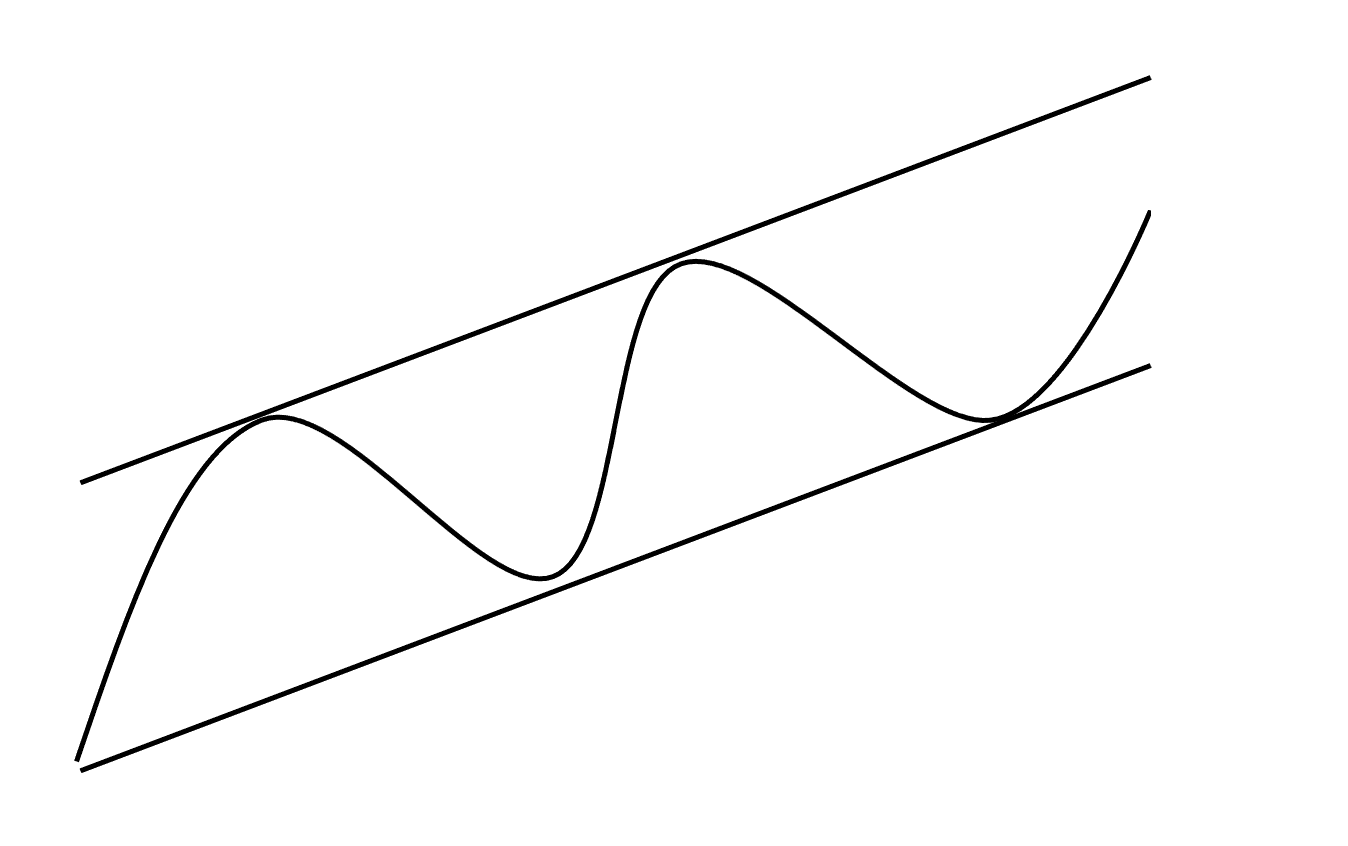
\includegraphics [scale=0.20,angle=360]{figures/trendup.png}
%\caption{Illustration of a Neural Network}
\label{fig:trendup}
\end{figure}
  \item \textbf{Falling trend} - stocks that are in a falling trend channel yield annual below-average returns of 11.4\% in the medium long term.
\begin{figure}[H]
\centering
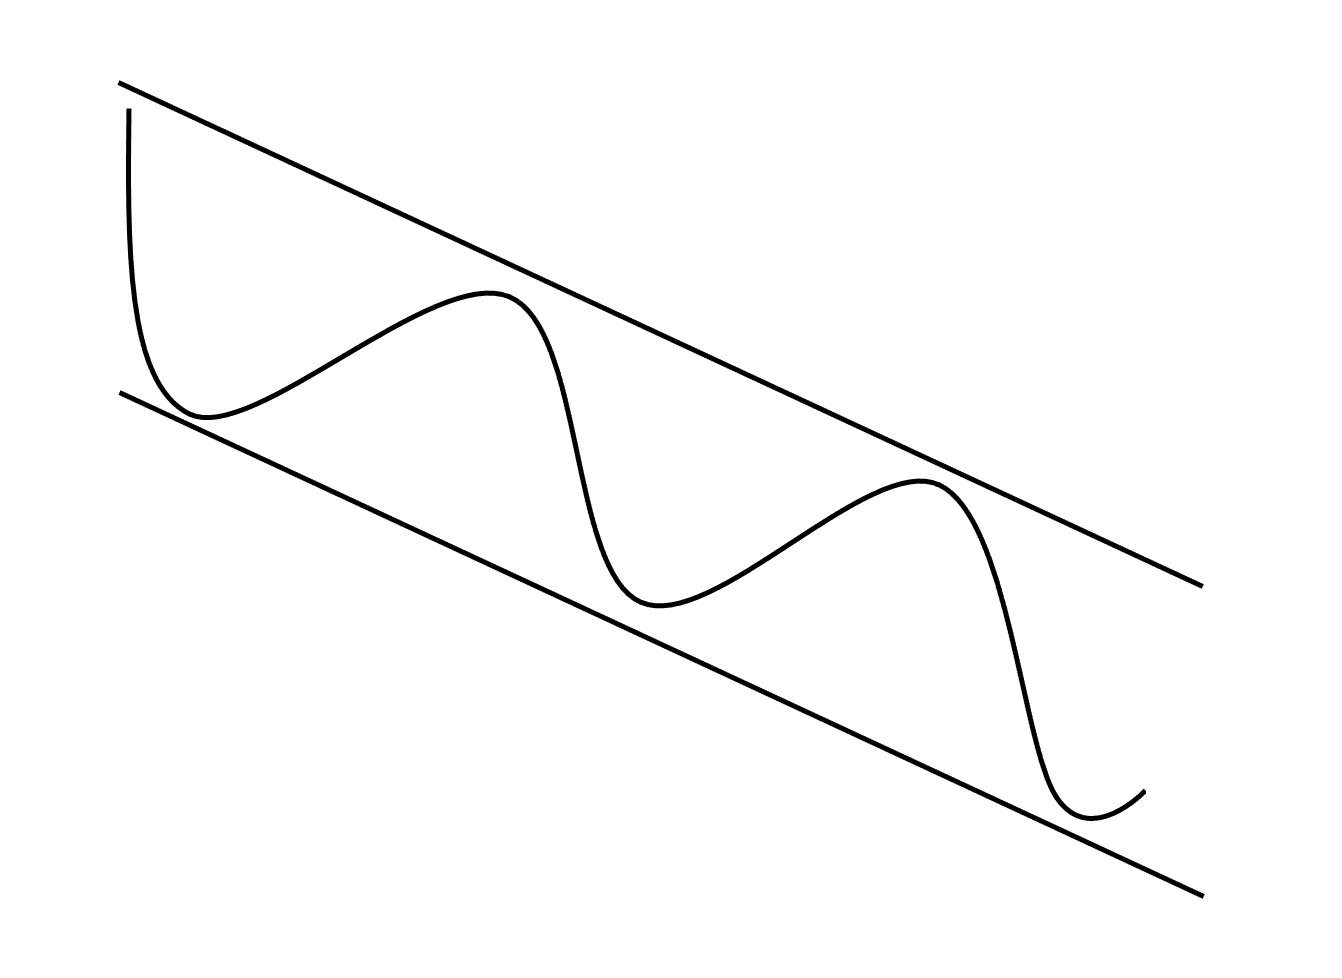
\includegraphics [scale=0.20,angle=360]{figures/trenddown.png}
%\caption{Illustration of a Neural Network}
\label{fig:trenddown}
\end{figure}
  \item \textbf{Trend break up} - stocks in rising trend channels which break up through the ceiling of the channel yield 14.7\% in annual excess returns in the medium long term.
\begin{figure}[H]
\centering
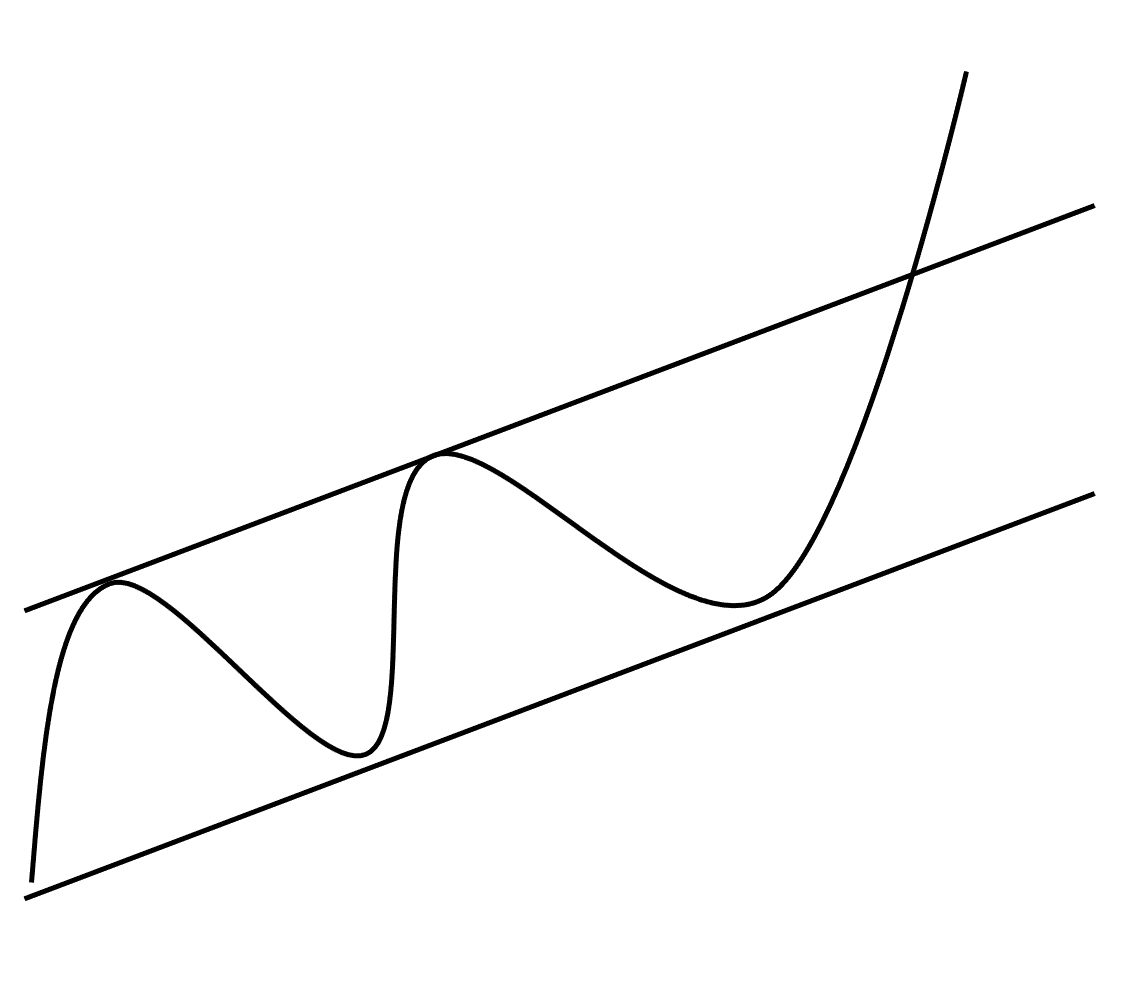
\includegraphics [scale=0.20,angle=360]{figures/breakup.png}
%\caption{Illustration of a Neural Network}
\label{fig:breakup}
\end{figure}
  \item \textbf{Trend break down} - stocks in falling trend channels which break down through the channel floor yield 27.9\% in annual below-average returns in the medium long term.
\begin{figure}[H]
\centering
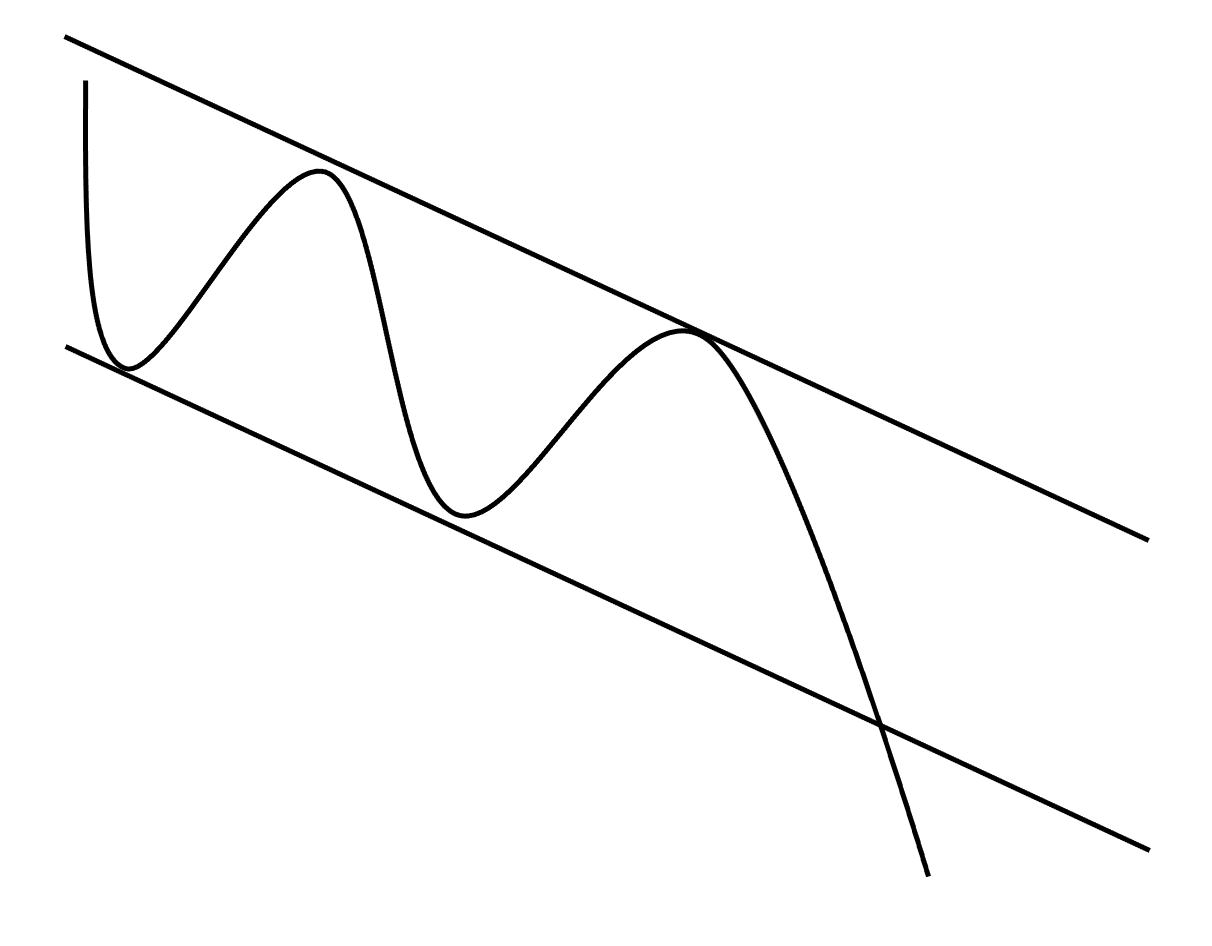
\includegraphics [scale=0.20,angle=360]{figures/breakdown.png}
%\caption{Illustration of a Neural Network}
\label{fig:breakdown}
\end{figure}
  \item \textbf{Positive volume balance} - stocks with a positive volume balance yield annual excess returns of 4.7\% in the medium long term.
\begin{figure}[H]
\centering
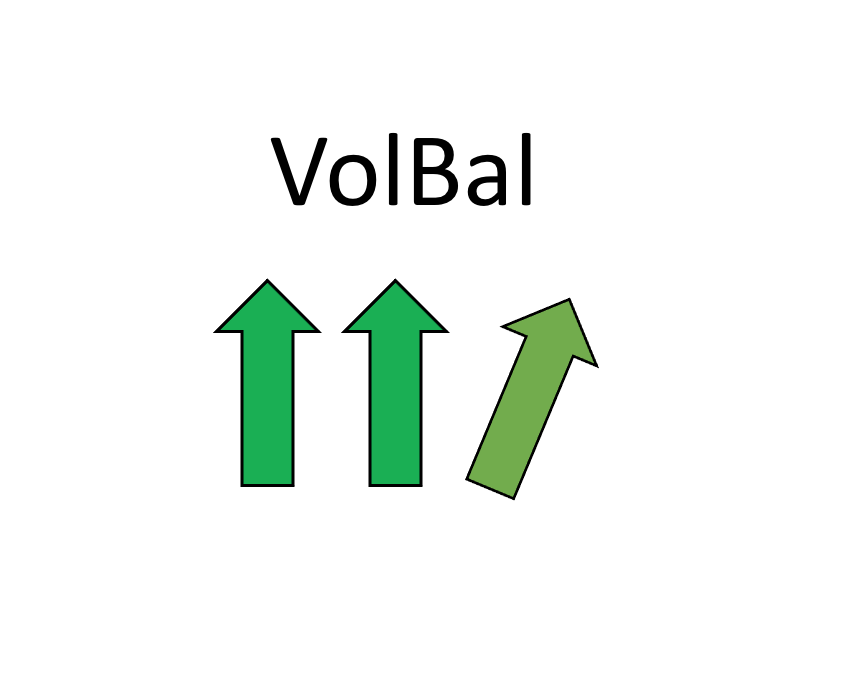
\includegraphics [scale=0.20,angle=360]{figures/volumepos.png}
%\caption{Illustration of a Neural Network}
\label{fig:volumepos}
\end{figure}
  \item \textbf{Negative volume balance} -  stocks with a negative volume balance yield annual below-average returns of 7.6\% in the medium long term.
\begin{figure}[H]
\centering
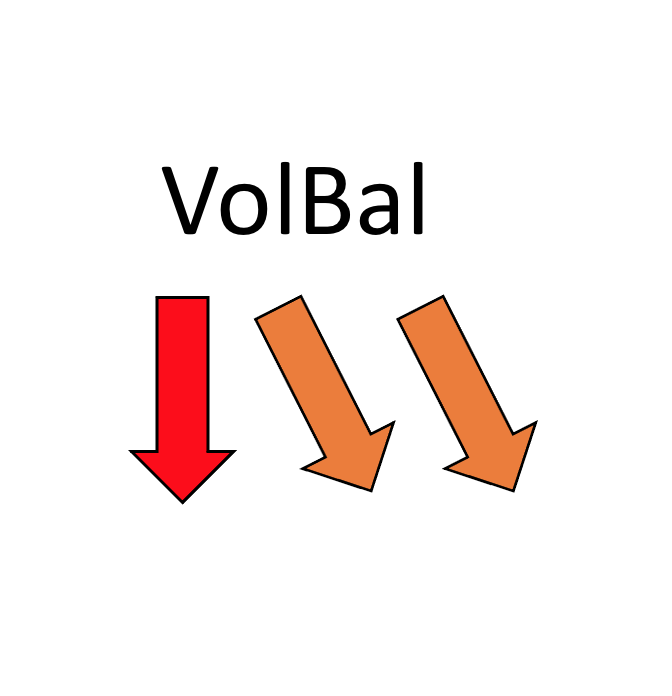
\includegraphics [scale=0.20,angle=360]{figures/volneg.png}
%\caption{Illustration of a Neural Network}
\label{fig:volneg}
\end{figure}
  \item \textbf{Strong positive momentum} - stocks with strong positive momentum yield 11.4\% in annual excess returns in the medium long term.
\begin{figure}[H]
\centering
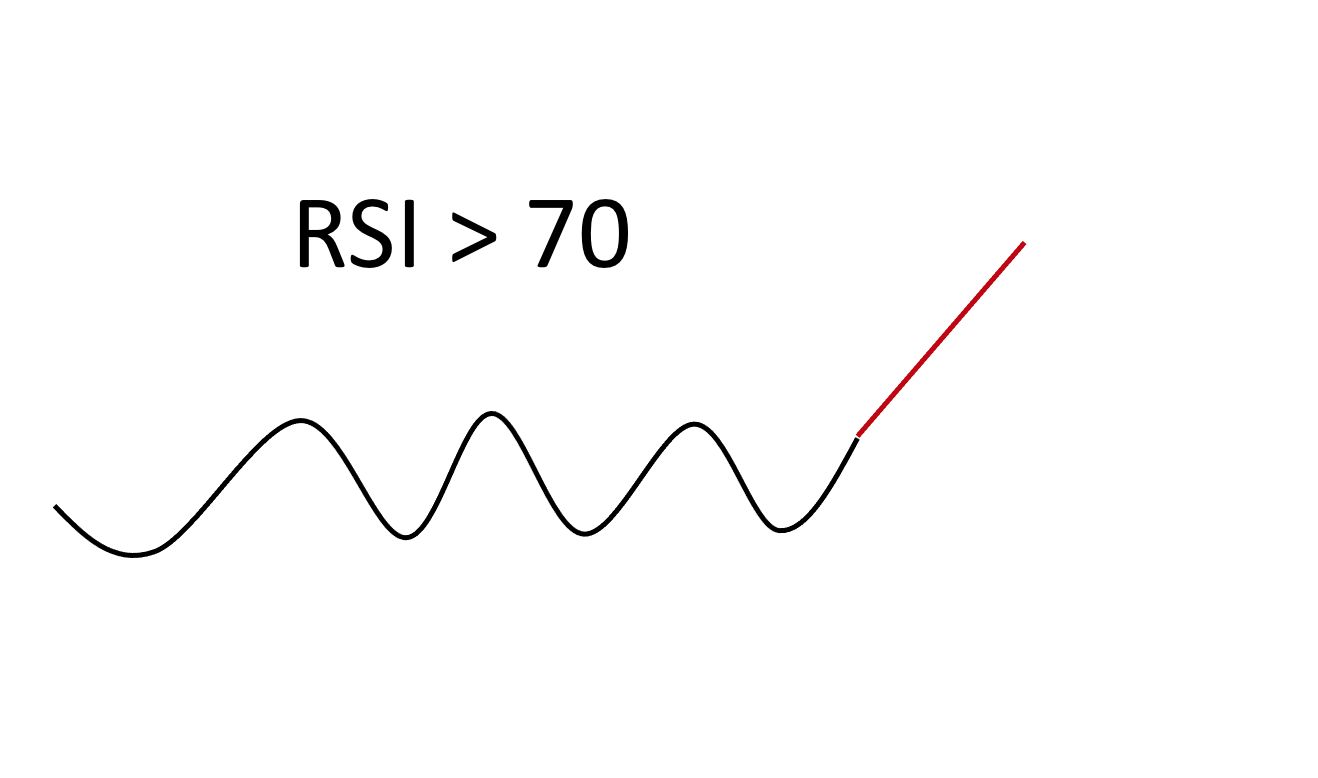
\includegraphics [scale=0.20,angle=360]{figures/momentumpos.png}
%\caption{Illustration of a Neural Network}
\label{fig:momentumpos}
\end{figure}
  \item \textbf{Strong negative momentum} - stocks with strong negative momentum yield 13.3\% in annual below-average returns in the medium long term. 
\begin{figure}[H]
\centering
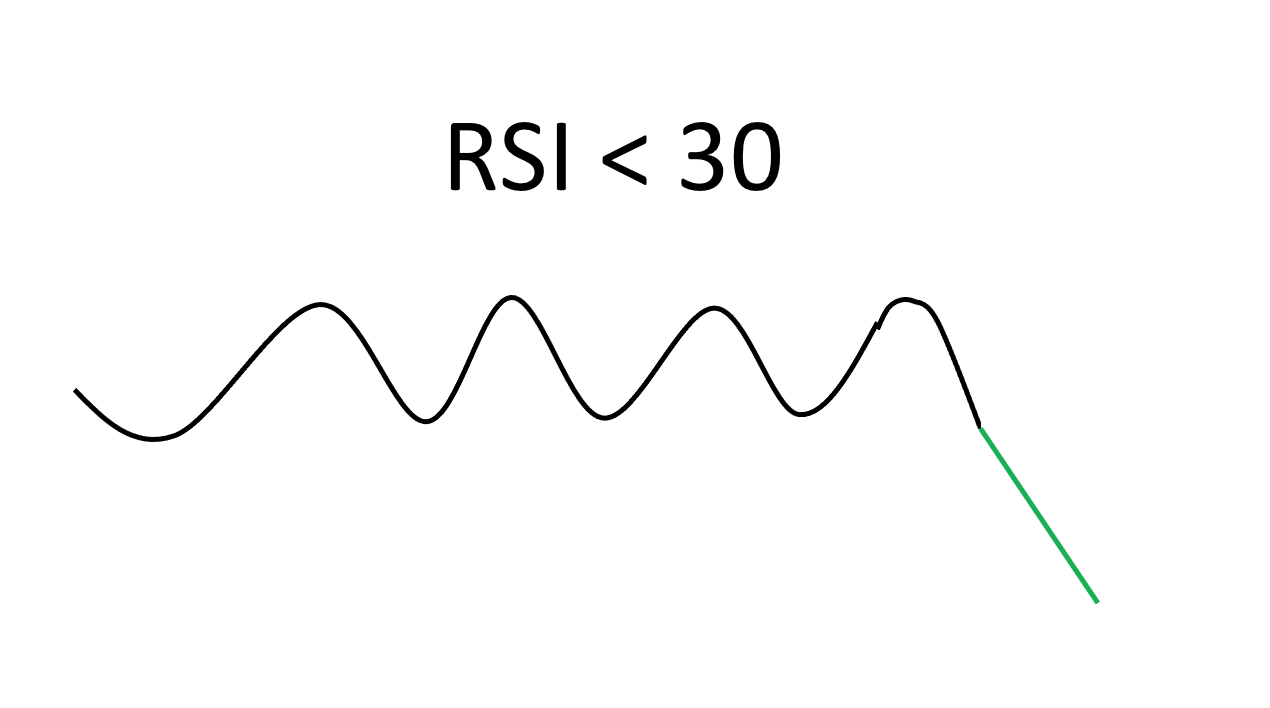
\includegraphics [scale=0.20,angle=360]{figures/momneg.png}
%\caption{Illustration of a Neural Network}
\label{fig:momneg}
\end{figure}  
\end{itemize}
\indent \newline 
\cite{investtech}

\indent \newline 
There are numerous different indicators and measures within the field of technical analysis, and the importance of each one varies greatly between investors. However, the main object of this type of investing strategy is to capture both the market psychology as a whole and also for individual stocks. Investors who utilize technical analysis seek to identify levels of a stock price where there are likely more buyers than sellers (will often lead to an increase in price) and levels where there are likely more sellers than buyers (will often lead to a decrease in price). A simplified explanation of the directional movements in price consists therefore of stock prices being greatly dependent on supply and demand. The level of aggressiveness among buyers and sellers is another factor which affects the movements of a stock price, and captures the psychological state of mind of the investors. Sellers who close their position by aggressively selling at bid, represent a situation where there is little optimism among investors and a probable decline in short-term price. Buyers who open positions by aggressively buying at ask, represents a situation where there is a lot of optimism among the investors and anticipations of a short-term increase in the stock price. 

\indent \newline 
Investors (traders) who base their investing strategy on technical analysis believe that the market psychology can be found in historical charts, prices and other technical measures, and that history repeats itself. An example of this is if a stock has previously reversed when falling to a certain price level on multiple occasions, the chances are that this will happen again. This is called a support level and represents a situation where there are many investors who believe the stock is cheap, and few sellers because they feel the stock is undervalued. Hence, there is a high probability that the stock price will increase based on a revitalized optimism among the investors again. This is under the assumption that there has not been any fundamental news that changes the company's future outlook.    

\indent \newline 
In order for technical analysis to work as either an investing strategy or investing tool, there must exist patterns within historical data that can be taken advantage of. If investors, through the use of technical analysis, are able to achieve above-average returns, it means that there must exist certain inefficiencies and that the weak form of the efficient market hypothesis does not hold. Instead of manually having to search for and detect these inefficiencies, this paper aims to utilize deep learning algorithms as an automated substitute for finding patterns within the data, representing potentially valuable entry points and ultimately above-average returns. Theory on deep learning is explained in the next section.          


\section{Machine Learning}
Modern enterprises today utilize the power of machine learning and computational power to assist every day-operations and operational decisions. Implementing analytics as an automated decision tool throughout the entire organization was previously characterized by tech-companies like Google, Amazon, Facebook etc, but in recent years this trend has changed. More and more mainstream companies are trying to replicate the success of these tech-companies by developing predictive models, visualization models, and other types of data-driven models to support operational decisions. Even though analytics and machine learning just recently has started to be recognized as a business asset, and not just a separate business project, the concepts of machine learning have been around for many years.  

\subsection{History}
Machine learning is partly based on the brain cell interaction-model created in 1949 by Donald Hebb in the book titled "The Organization of Behaviour". Hebb presented theories on neuron excitement and communication between neurons, which can be translated into the concepts of artificial neural networks and artificial neurons \cite{dataversity}. In the 1950’s Arthur Samuel came up with the phrase "Machine Learning". He developed a chess computer program based on alpha-beta pruning, where the program chooses the next move by using a minimax strategy and a scoring function. Samuel introduced rote learning, where the program recorded all previous positions and combined this with the reward function. In the same decade, Frank Rosenblatt built upon the work of Hebb and Samuel by creating the perceptron. The program was designed for image recognition. However, the program did not produce satisfying results, where it was only able to recognize a few kinds of visual patterns. This led to a stagnation in the research of machine learning and neural networks, which lasted until the 1990's. 

\indent\newline
In 1967, Marcello Pelillo was given credit for developing the nearest neighbour algorithm. The algorithm was developed in connection with the traveling salesperson's problem, where the algorithm was used for mapping routes and finding the most efficient one. This is considered as the beginning of basic pattern recognition. Further in the same decade, multilayers were introduced in the research of neural networks. Using more than one layer in the perceptron resulted in a significant increase in processing power, which laid the foundation for the future development of feedforward neural networks and backpropagation. The backpropagation algorithm differs from feedforward neural networks by having the ability to process output errors and distribute them backwards through the layers of the network. This improves the learning ability of the network and is currently being used to train deep neural networks \cite{dataversity}. 

\indent\newline
During the period from the 1970's and 1990's the fields of machine learning and artificial intelligence were separated. Machine learning had previously been incorporated as a training program for artificial intelligence, but shifted focus to solve more service-oriented tasks during this period. Machine learning flourished in the 1990's as a result of the internet growth and focus on neural networks. Increased access to digital data and an easier ability to share data and services was the main reasoning behind the revived success of machine learning during this decade. In this decade, Robert Schapire introduced the concept of boosting. This is a technique developed to reduce bias during supervised learning and to transform weak learners into strong learners. Boosting algorithms create a final strong classifier by repetitive learning weak classifiers. Each weak classifier is weighted based on the learner’s accuracy and then reweighted. The weight of misclassified input data increases, while the weight of correctly classified data decreases, in order for future weak learners to focus more on previous misclassified weak learners. Strong learners are easily classified aligned with the true classification, while weak learners are only slightly correlated with the true classification \cite{dataversity}. 

\indent\newline
Ever since the millennium, machine learning has been applied to several business areas. In the early 2000's, speech and facial recognition technology was developed. Speech recognition is based on Long Short-Term Memory (LSTM), which is a neural network technique developed by Jürgen Schmidhuber and Sepp Hochtreiter in 1997. LSTM is particularly relevant for speech recognition in terms of being able to learn tasks that require the model to be able to memorize discrete steps that took place thousands of steps earlier. The relevance of the model was highlighted in 2015 when Google's speech recognition program gained a 49\% increase in performance by using a LSTM model. During the same period, newly developed facial recognition algorithms were found to be 10 times more accurate than algorithms from 2002 and 100 times more accurate compared to algorithms applied in 1995 \cite{dataversity}.    

\indent\newline
Today, machine learning is considered as the computer's ability of making automated actions without being explicitly programmed. The applicability of machine learning is relevant for several business areas, which include:
\indent \newline
\begin{itemize}
\item {\textbf{Self-driving vehicles} - Autonomous cars are currently being developed with the use of machine learning and deep learning. These cars have the ability to steer, accelerate and brake, based on prior knowledge, stimuli and past experiences. Prior knowledge includes street maps, the meaning of signs, what to stop for etc. Stimuli are made up of a combination of sensors like vision, lidar, radar, GPS and voice commands, while past experiences can for example be how braking and steering affects direction and speed.  where prior knowledge like street maps, meaning of signs, what to stop for etc.}
\item {\textbf{Business decisions} - Machine learning is increasingly being used for operational decisions, which covers various business operations like predicting production metrics, the number of new customers based on marketing campaigns, or predicting inventory based on customer demand.}
\item {\textbf{Fraud detection} -Fraud related to tax evasion, money laundering and insurance are common problems for most countries, and cost governments billions of dollars each year. By implementing machine learning and predictive models, governments are now able to prevent and detect fraud in a much more efficient way.}
\item {\textbf{Natural language processing} - Machine learning enables Email filtering, where algorithms are able to detect spam and recognize different categories the Email belongs to. Other examples of natural language processing include smart assistants, improvement in search results where search engines are able to give relevant results based on similar search behaviour, and predictive text like autocorrect and autocomplete.}
\end{itemize}

\indent\newline
Within finance, there is an increasing amount of hedge funds that are utilizing machine learning to get an edge over the broad market. Hedge funds use it as support to anticipate market movements and detect market trends at an early stage. Machine learning models also help them get a better understanding of how specific news will affect the market direction and intensity. The main point by incorporating machine learning in this field is to be able to extract information out of large amounts of data. This can for example be to use satellite data to determine customer traffic in retail or to calculate the level of crude oil storage, or to use natural language processing to analyze market sentiment through large amounts of text related to important macroeconomic factors.    

\section{Deep Learning}
In the field of artificial intelligence, deep learning is a subset of machine learning where neural networks can identify patterns within training data, where they eventually are able to make predictions from new, unseen data. The structure of deep learning is based on the workings of a human brain, where the brain is used to recognize patterns and classify various types of information. Neural networks can be trained to perform several tasks, which include regression, classification and clustering \cite{opper}. Before going more into detail on the network structure and how the network learns, it is important to get an idea of how the human brain functions, which in turn can give a better understanding of how deep learning networks work in practice.

\subsection{Biological Neural Networks}
Artificial neural networks can be compared to biological neural networks in terms of artificial neural networks trying to simulate some of the functionalities of the neural networks in the human brain. The processes are quite similar, where artificial neural networks try to imitate the human brain's biological neurons, but in a more simplified way.  

\indent\newline
\begin{figure}[H]
\centering
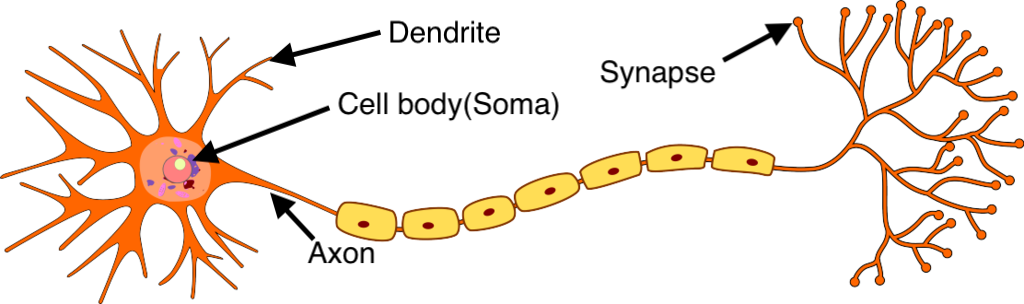
\includegraphics [scale=0.34,angle=360]{figures/bio.png}
\caption{Illustration of a Neuron (source: Wikimedia Commons)}
\label{fig:bio}
\end{figure}
 
\indent\newline   
The figure above illustrates the workings of a nerve cell (neuron) in the human brain. The neurons are arranged together to form a network of nerves, where they transmit and process information received from human senses. These are electrical impulses being passed from one neuron to another. Impulses from the synapse of an adjoining neuron are received through the part of the neuron termed dendrites. The impulses are then carried further to the nucleus (soma), where the electrical impulses are processed before being passed to the axon. The axon consists of a longer branch with a main function of carrying the electrical signal from the soma to the synapse. Lastly, the signal is passed to a neighboring neuron's dendrites, which creates an intricate network of neurons in the human brain \cite{panchal}.  The neurons are electrically excitable due to their membranes' maintenance of voltage gradients. A large amount of change in voltage, in a short amount of time, creates an action potential (electrical pulse) that travels rapidly through the axon and activates adjoining neuron's synaptic connections \cite{opper}.    

\subsection{Neural Network Structure}
As with linear regression, the data consist of independent variables \textit{$x_{n}$}, with an assumption that these features are able to explain the variability in the dependent variable \textit{y}. The target variable can either be continuous or categorical, depending on whether the network is a regression or classification model. Categorical dependent variables consist of a finite number of categories or groups. Examples of a classification model could be predicting gender, type of animals, if an email is spam or not, or classifying customer churn based on recent behaviour. Classification models normally consists of four types of classification, which include:

\begin{itemize}
\item {Binary classification} - This is a very common classification task consisting of having two class labels, where one class represents the normal state and the other class the abnormal state. The class representing the normal state is assigned the value 0, while the class representing the abnormal state is assigned the value 1. Binary classification models usually include a discrete probability distribution, where the models predict the probability of an observation belonging to the two classes.
\item {Multi-class classification} - This type of classification refers to tasks where there are more than two class labels. This means that there could be thousands of known classes, as for example would be the case in face recognition. Normally, a multinoulli probability distribution is incorporated in the predictive model, where the model predicts the probability of an observation belonging to each of the several class labels.
\item {Multi-label classification} - In this case, there are at least two class labels, where the classification task may require predicting more than one class label for each observation. This might be the case in photo classification, where there could potentially be several objects (class labels) in one photo (observation). Also in this type of classification task, it is common to incorporate a discrete probability distribution, where the model predicts multiple outputs and multiple binary classification predictions for each observation.
\item {Imbalanced classification} - The last type of the most common classification problems is imbalanced classification. This type of classification refers to tasks where the number of observations in each class are unequally distributed and where most of the observations belong to the normal class label. A common technique to solve these types of problems consists of combining a normal binary classification model with either undersampling the majority class or oversampling the minority class.
\end{itemize}
\cite{brownlee} 

\indent\newline
Continuous dependent variables have infinite numeric values, which can also consist of date or time. Examples of regression (continuous output) could be predicting next month's sales, traveling time for a specific route, or the number of new customers based on a marketing campaign. In linear regression, coefficients for the independent variables are estimated to make predictions for the target variable, while neural networks incorporate non-linearity and a more intricate structure to gain a deeper understanding of patterns within the data. 

\indent\newline 
\begin{figure}[H]
\centering
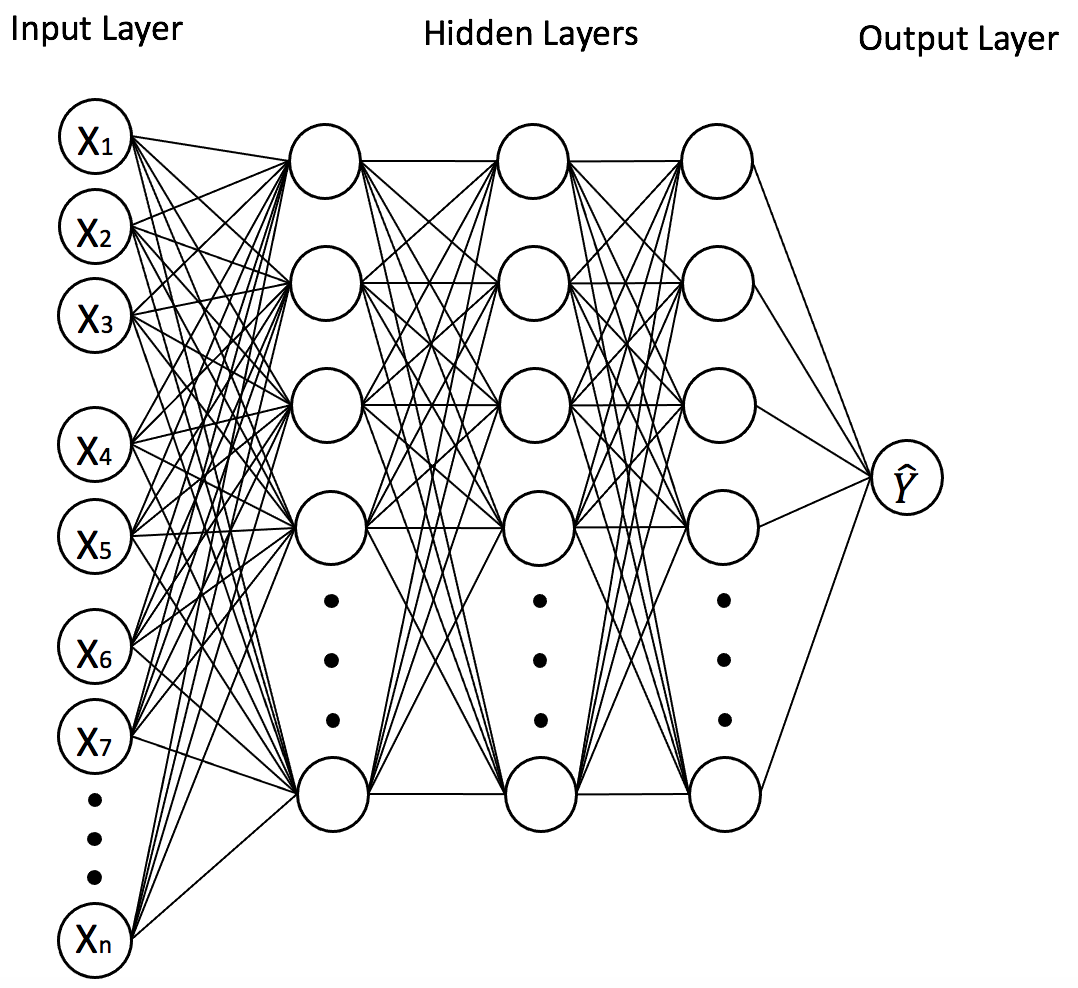
\includegraphics [scale=0.60,angle=360]{figures/neur.png}
\caption{Illustration of a Neural Network}
\label{fig:neur}
\end{figure}

\indent\newline
Figure 2.2 illustrates a traditional neural network, where the nodes represent artificial neurons. These can be compared to the biological neurons of the human brain. The nodes are a graphical representation of numeric values, while the connections can be thought of as the axons in the biological neuron. These connections have different dynamic weights that change as the network trains to learn the patterns within the data. The strength of the connections also changes with an aim for the network to set the right weights, in order to make accurate predictions \cite{opper}. The layers of the neural network can be divided into an input layer, hidden layers and an output layer. The input layer is where the network receives the input data \textit{x}, which consist of features considered to have an explanatory effect on the dependent variable. Each \textit{x} is an entire vector where an input neuron represents one element in the vector. The hidden layers are where mathematical operations are performed in order for the neural network to obtain a prediction vector \textit{y}. Lastly, the output layer is where the network's predictions are being made. An output neuron consists of the value of the prediction, which is a vector \textit{y}. The values presented in this layer could either be a probability value between 0 and 1 (classification) or an infinite value predicting a desired target value (regression) \cite{opper}. 

\indent\newline 
\begin{figure}[H]
\centering
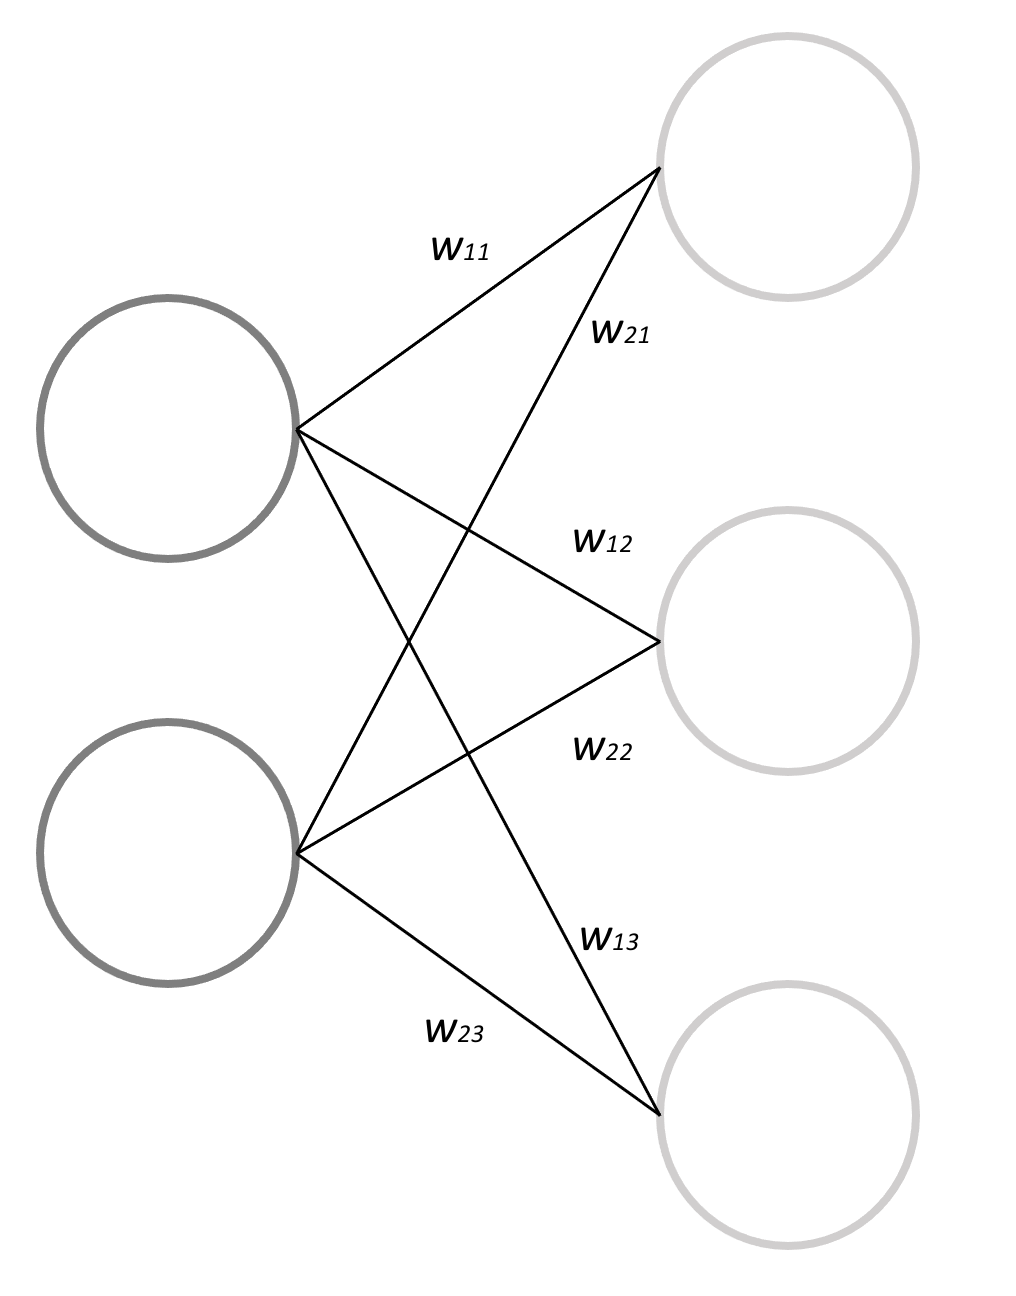
\includegraphics [scale=0.40,angle=360]{figures/weights.png}
\caption{Weights in a Neural Network}
\label{fig:weights}
\end{figure}

\indent\newline 
Figure 2.3 shows an example of a simple neural network with an input layer consisting of two neurons and an output layer with 3 neurons. Each connection between two neurons is represented by a weight w, where each weight has indices. The first number of indices tells us the number of neurons from the connection's origin, while the second value tells us the number of neurons in the layer where the connection leads. The weights between the layers of a neural network can be illustrated through a weight matrix, which is shown below. 
\indent\newline 
\begin{center}
\textit{W} = $\begin{pmatrix}
w_{11} & w_{12} & w_{13}\\
w_{21} & w_{22} & w_{23}
\end{pmatrix}$
\end{center}

\indent\newline 
The number of entries in a weight matrix corresponds to the number of connections between neurons. This means that the dimensions of the matrix is determined by the layers' size and their connections. The weight matrix above has two rows, since there are two neurons in the input layer and three columns because of the three neurons in the output layer \cite{opper}.

\subsection{The Learning Process}
Having established the basic concepts and structures of a neural network, this section will look at how the network learns. Forward propagation consists of the step where the neural network performs a prediction vector based on an input feature vector \textit{x}. The prediction vector will here be termed as \textit{h}. The dot product of the weight matrix \textit{W} (explained in the previous section) and the input vector \textit{x} is then computed, which gives the vector \textit{z}.

\indent\newline 
$\overrightarrow{x}^{T} \cdot W$ = $\begin{pmatrix} x_{1}, & x_{2}
\end{pmatrix} \cdot \begin{pmatrix}
w_{11} & w_{12} & w_{13}\\
w_{21} & w_{22} & w_{23}
\end{pmatrix}$
  
\indent\newline 
= $\begin{pmatrix}
x_{1}w_{11}+x_{2}w_{21}, & x_{1}w_{12}+x_{2}w_{22}, & x_{1}w_{13}+x_{2}w_{23}
\end{pmatrix}$

\indent\newline 
= $\begin{pmatrix}
z_{1}, & z_{2}, & z_{3}
\end{pmatrix}$ = $\overrightarrow{z}, \overrightarrow{h}$ = $\sigma(\overrightarrow{z})$

\indent\newline 
In order to obtain the prediction vector \textit{h}, one of three non-linear activation functions is applied to the dot product vector \textit{z}. The three activation functions can be either tanh, sigmoid or ReLu, which enables a non-linear mapping from \textit{z} to \textit{h}. This allows the network to understand non-linear data through the linear combination value of the weights and neurons and the non-linear activation function.

\indent\newline 
The last part of the learning process of the neural network, and the last step in forward propagation, consists of computing a loss function \textit{L}. This phase consists of comparing the prediction vector \textit{y} with the ground truth $\widehat{y}$. The ground truth label represents the actual values, where the difference between the values of $\widehat{y}$ and the predicted values \textit{y} are computed in order to measure the network's accuracy. Minimizing the loss function \textit{L} enables the network to learn and adjust the weights accordingly, as the distance between \textit{y} and $\widehat{y}$ is revealed to the  network. In other words, the network is able to learn how the parameters $\theta$ contribute to the loss function and how it should change these parameters in order to decrease the distance between $\widehat{y}$ and \textit{y}.

\indent\newline 
Two of the most common loss functions implemented in deep learning are the mean squared error loss and the cross-entropy loss. 

\indent\newline 
\textbf{Mean squared error loss:}

\indent\newline 
$L(\theta) = \frac{1}{N} \sum_{i=0}^{N} (y_{i} - \widehat{y}_{i})^{2}$

\indent\newline 
Where,
\indent\newline 
$y_{i}$ = entries in the prediction vector $\overrightarrow{y}$
\indent\newline 
$\widehat{y_{i}}$ = entries in the ground truth label $\widehat{\overrightarrow{y}}$

\indent\newline 
\textbf{Cross-Entropy Loss:}

\indent\newline 
$L(\theta) = - \sum_{i=0}^{N} \widehat{y_{i}} \cdot log(y_{i})$

\indent\newline 
Where,
\indent\newline 
$y_{i}$ = entries in the prediction vector $\overrightarrow{y}$
\indent\newline 
$\widehat{y_{i}}$ = entries in the ground truth label $\widehat{\overrightarrow{y}}$

\indent\newline 
\cite{opper}.

\indent\newline 
Minimizing the loss function is solved mathematically by the method termed gradient descent. The method involves taking the derivative of the loss function where each gradient descent step enables the network to get closer in optimizing the weights, and ultimately make satisfying predictions. A simplified example would be a neural network with one input neuron, one output neuron and one connecting weight value, where the network first performs an inaccurate prediction based on a certain weight value. To improve the accuracy a loss function needs to be chosen (in this case a quadratic loss function) where the gradient descent method will update the weight with a more correct value. 

\indent\newline 
\begin{figure}[H]
\centering
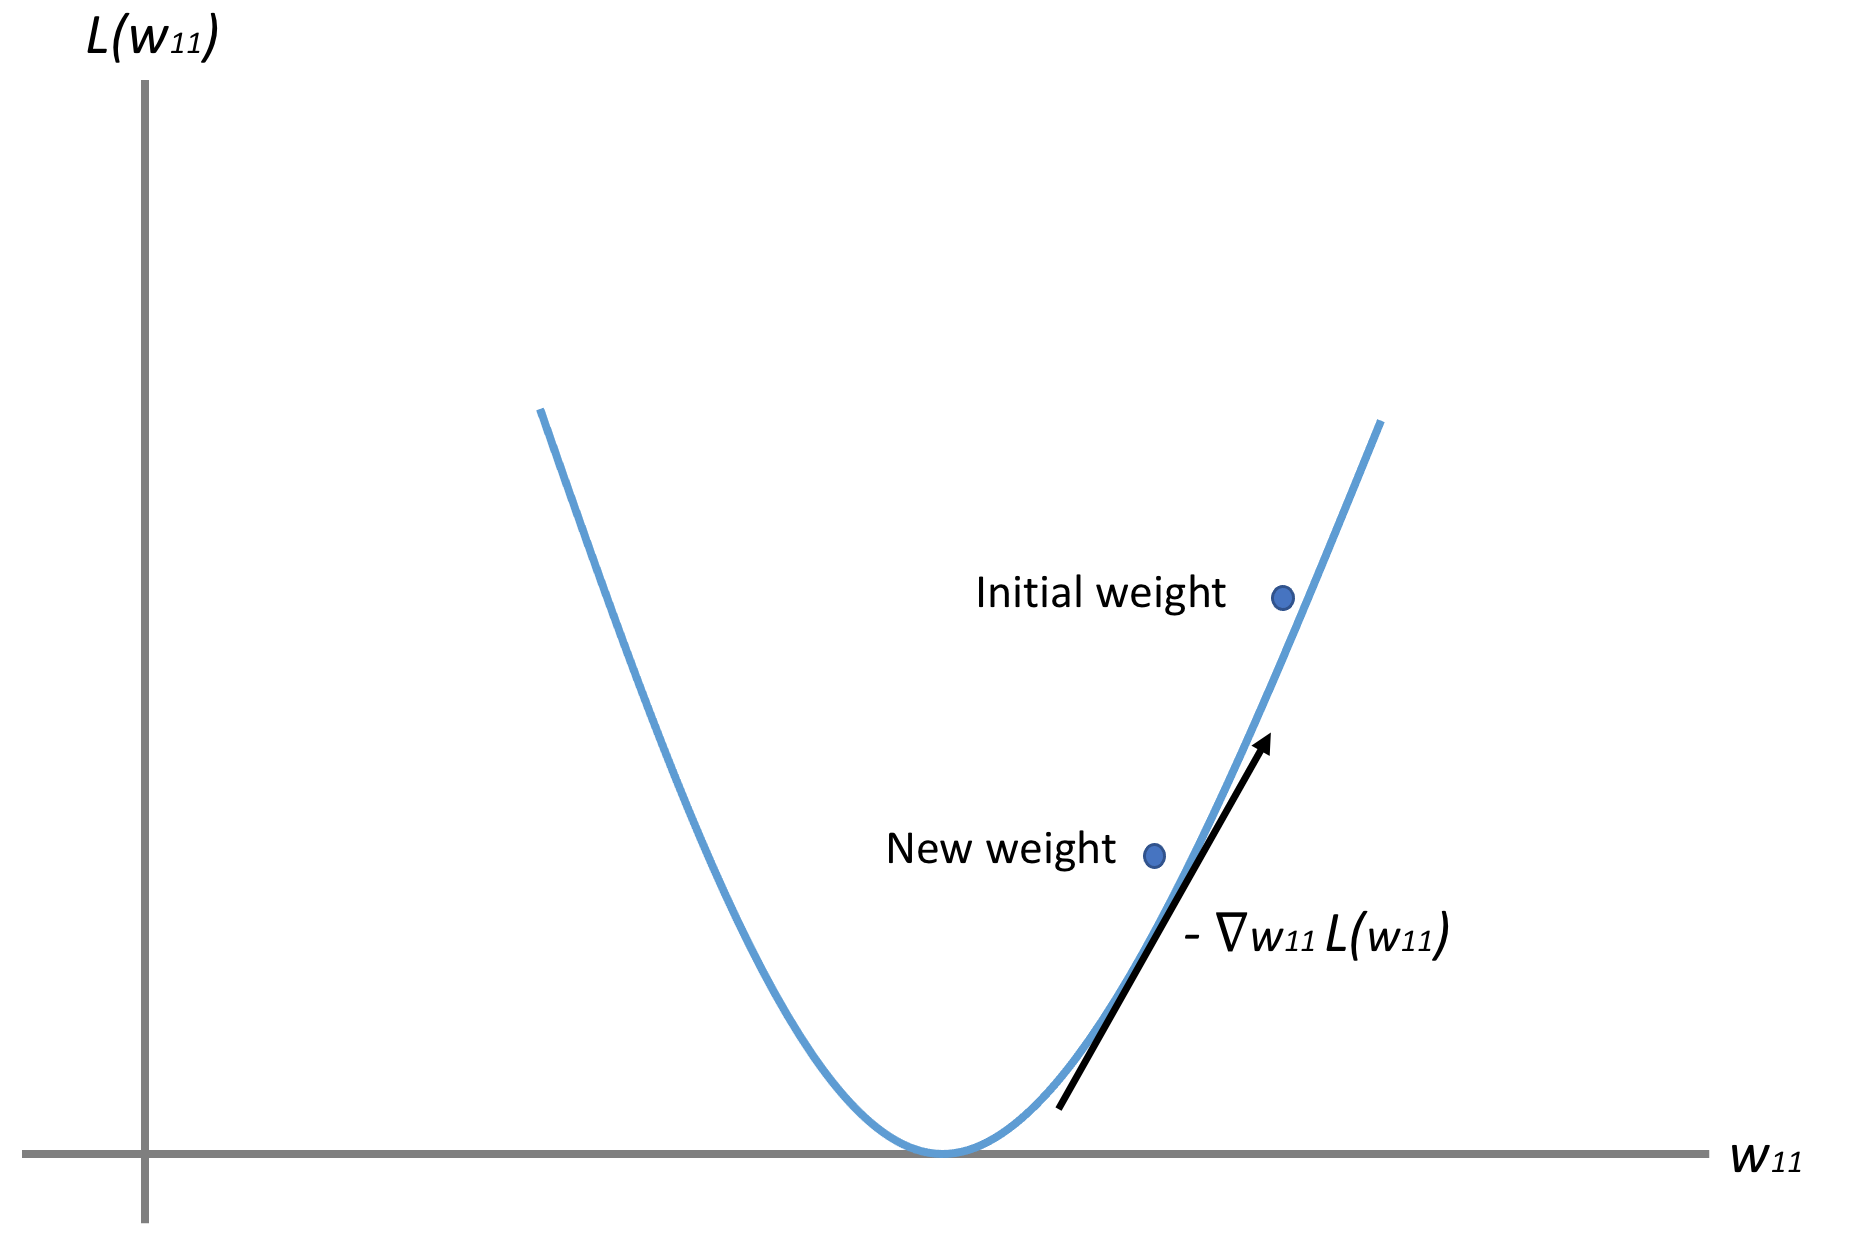
\includegraphics [scale=0.40,angle=360]{figures/gradient.png}
\caption{Gradient Descent}
\label{fig:gradient}
\end{figure}

\indent\newline 
The x-axis in figure 2.4 is the value of the weight, while the y-axis is the difference between the ground truth and the prediction, and essentially the network parameters (the value of the loss function). Using a quadratic loss function means that there is only a global minimum and not a local minimum. The global minimum represents the value of the weight that enables the network to make an accurate prediction, and is shown in the figure as the point where the loss function is equal to zero. In the fictive example shown in the figure, the initial prediction and weight value is relatively inaccurate. To improve the accuracy of the prediction, the next step involves updating the weight parameter until it reaches an optimized value for the weight. This is carried out by taking the derivative of the loss function with respect to the weight \textit{w}.

\indent\newline
$\nabla_{w11} L(w_{11}) = \frac{\partial L(w_{11})}{\partial w_{11})}$

\indent\newline
The equation computes the tangent (slope) of the loss function for the point of where the initial weight lies. The figure shows that the tangent of the loss function would be positive, which would correspond to the network updating the weights to a higher loss value and making even more inaccurate predictions. However, this can be solved by multiplying the gradient by minus one to get the opposite direction of the gradient.  

\indent\newline
$w_{11_{new}} = w_{11_{old}} - \epsilon \cdot \nabla_{w11} L(w_{11})$

\indent\newline
The equation above shows a step of the gradient descent where the network updates the value of the weight to make a more accurate prediction. In the equation, epsilon is implemented as the network’s learning rate and represents how quickly the parameters are updated. This method of updating the parameters continues until the loss function reaches a point of global minimum, which represents the optimal weight value for the network to perform accurate predictions \cite{opper}.  

\subsection{LSTM Network}
Unlike feed forward neural networks (FNNs) explained in the previous section, long short-term memory networks (LSTMs) is a type of recurrent neural network (RNN). Comparing RNNs with FNNs, RNNs resemble a more accurate representation of the workings of a biological neural network. The human brain has the ability to retain previous learnt information while receiving new information, which can either change a perceived outcome or it can remain unchanged. The same logic applies to RNNs, where loops within the networks are utilized to incorporate past information in the final output \cite{adu}. 

\indent\newline 
\begin{figure}[H]
\centering
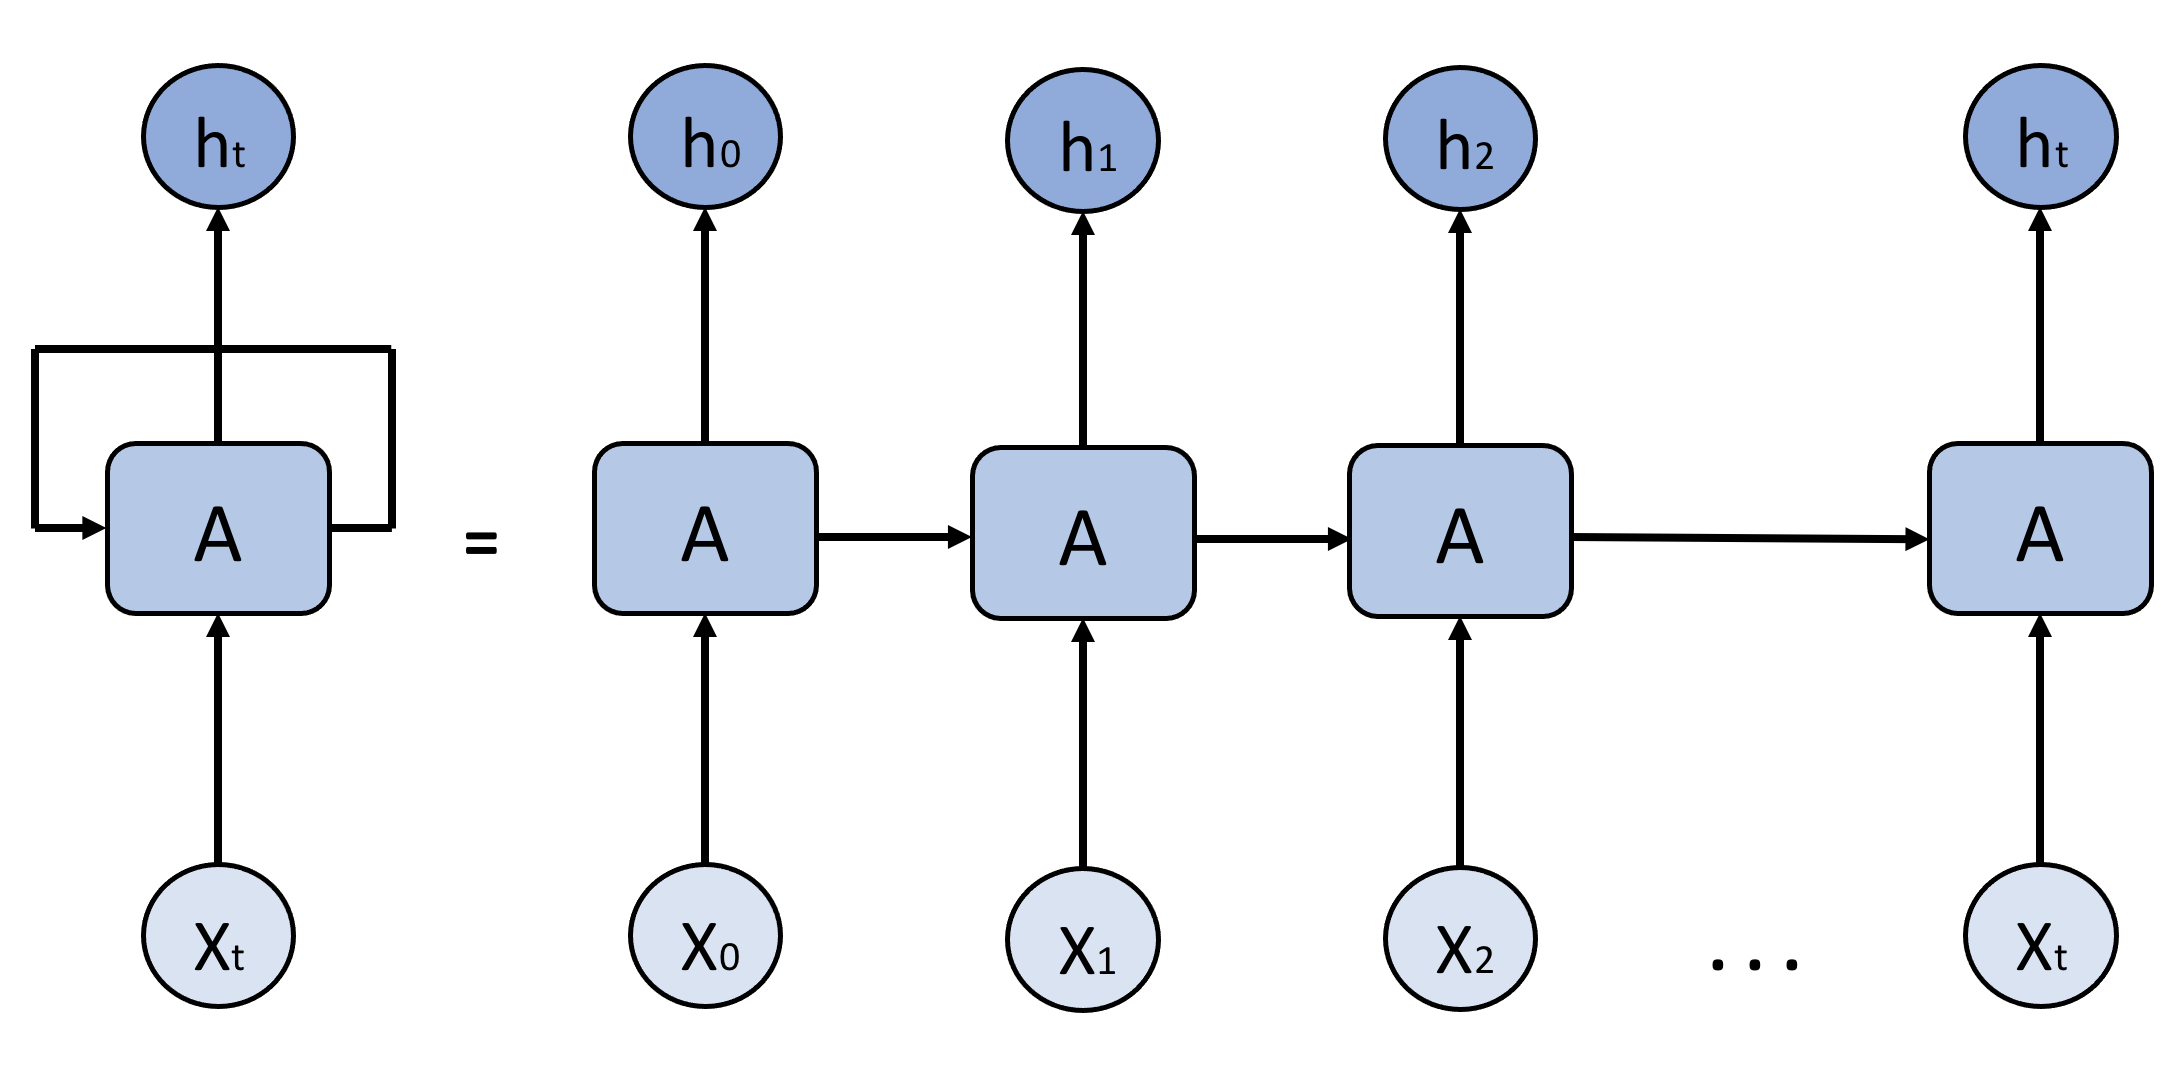
\includegraphics [scale=0.32,angle=360]{figures/rnn.png}
\caption{Structure of a Simple RNN}
\label{fig:rnn}
\end{figure}

\indent\newline 
Figure 2.5 illustrates a simple RNN where \textit{A} represents a piece of neural network (repeating module), $X_{t}$ is some input, $h_{t}$ an output value, while the loop allows the network to pass information from each step to the next. The right side of the figure illustrates a recurrent neural network if it had been unrolled, and demonstrates a chain-like characteristic useful for data consisting of sequences and lists \cite{olah}.    

\indent\newline 
A limitation with simple RNNs is their ability to retain previous learnt information over longer periods of time. Their short-term memory is connected to the vanishing gradient problem \cite{phi}. During backpropagation, these simple RNNs' gradients shrink as they back propagate through time and their values become extremely small. This applies normally to the earlier layers when the update values become so small that the layers stop learning. This can make the RNNs forget what they have previously seen. In relation to predicting stock returns, LSTM is a type of RNN which can cope with this problem since financial time series requires predictive models to train on large data sets, stretching over a long period of time. 
\indent\newline 
\begin{figure}[H]
\centering
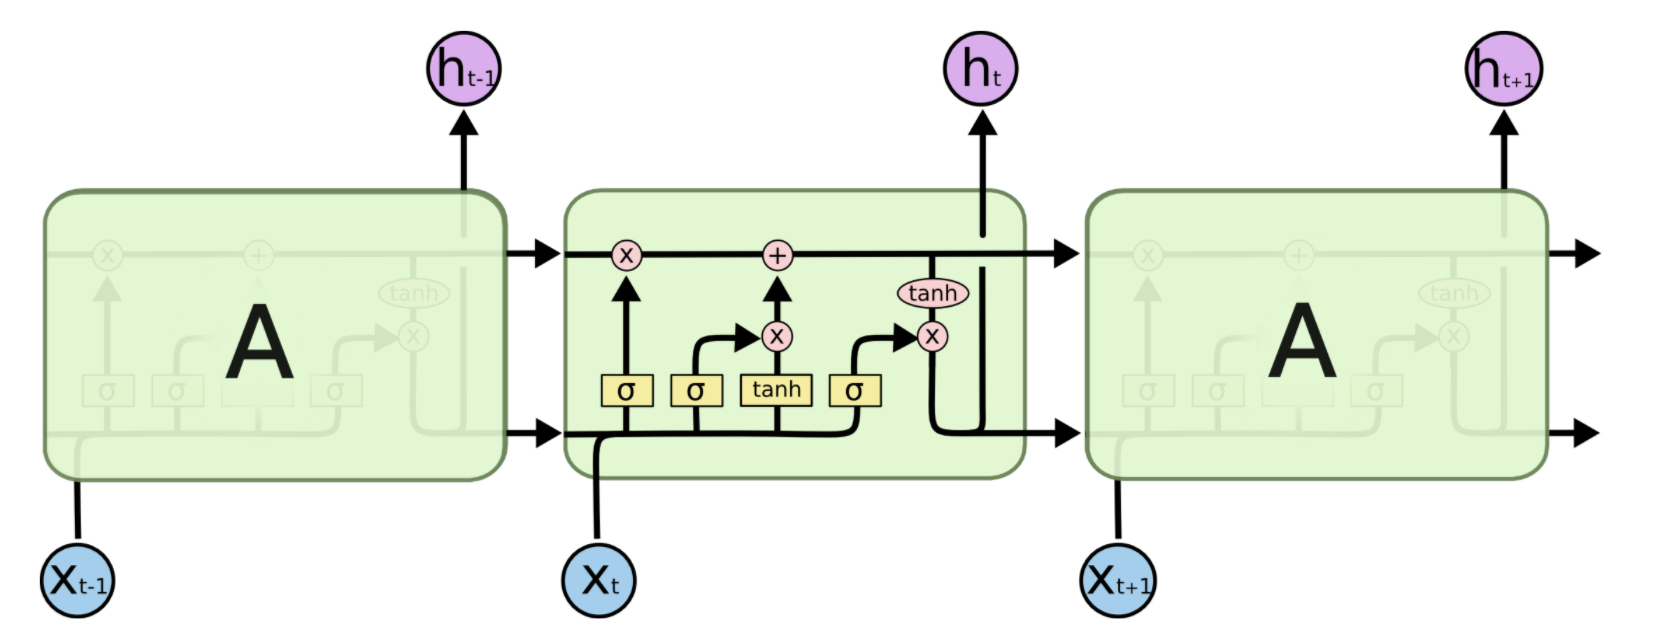
\includegraphics [scale=0.40,angle=360]{figures/lstm.png}
\caption{Structure of a LSTM-Network (source: \cite{olah})}
\label{fig:lstm}
\end{figure}

\indent\newline 
Figure 2.6 illustrates the recurrent system of an LSTM. The yellow boxes represent learned network layers, the pink circles are pointwise operations, while each line visualize how the LSTM carries entire vectors. Merging lines depict concatenation and lines that fork is a representation of copied contents going to other locations \cite{olah}. 

\indent\newline 
\begin{figure}[H]
\centering
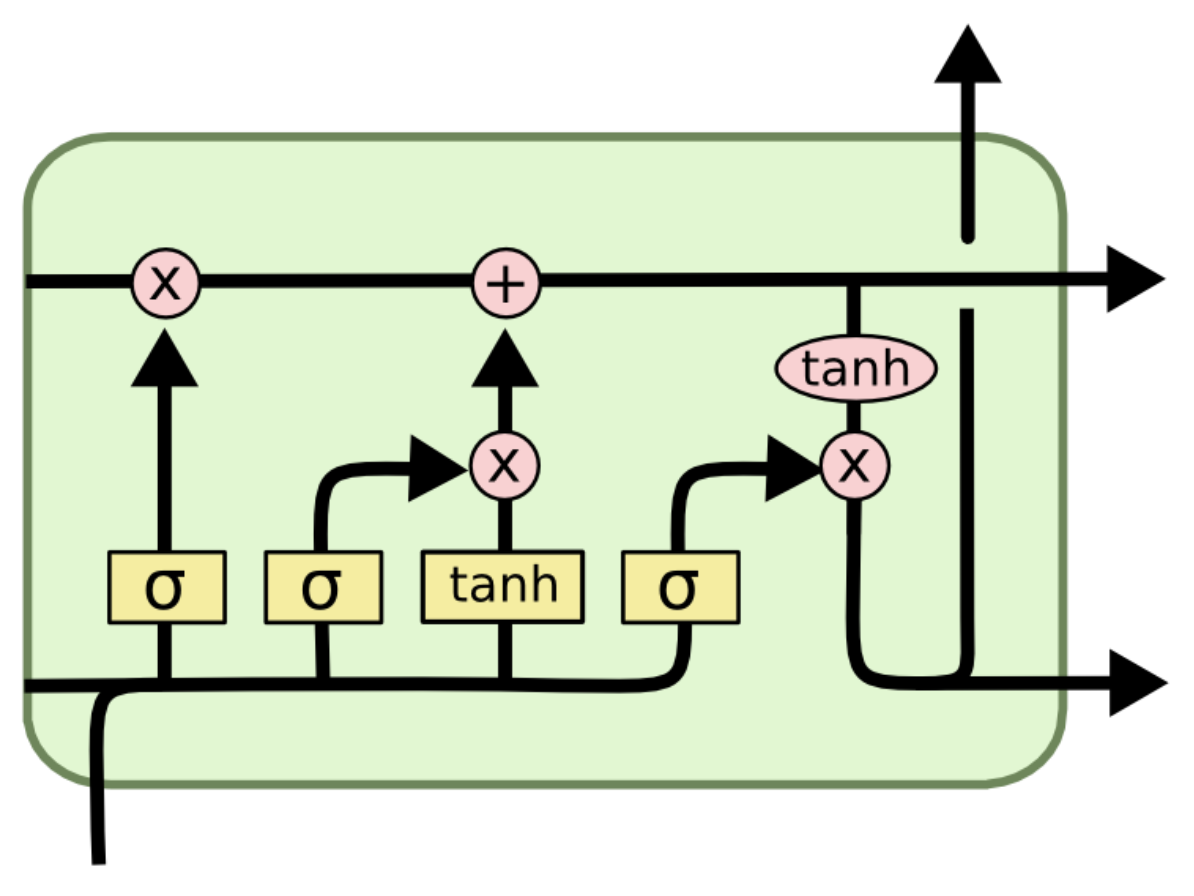
\includegraphics [scale=0.40,angle=360]{figures/module.png}
\caption{The Repeating Module (source: \cite{olah})}
\label{fig:module}
\end{figure}

\indent\newline 
One of the main differences between a simple RNN and an LSTM is the repeating module. A standard RNN only has a single neural network layer, while an LSTM has four interacting neural network layers. The horizontal line running through figure 2.7 illustrates the cell state $C_{t}$. This represents the flow of information through the network chain. In order for the LSTM to regulate the information being passed through, three different types of gates are used. The gates are made up of a neural network layer and a pointwise multiplication operation, and consist of a forget gate $f_{t}$, an input gate $i_{t}$, and an output gate $o_{t}$ \cite{olah}. The forget gate is a sigmoid layer that decides which parts of the information to forget. $f_{t}$ outputs a value between 1 and 0 for each number in the cell state $C_{t-1}$ by evaluating $h_{t-1}$ and $x_{t}$, where a value of 1 means keeping all of the information and a value of 0 means forgetting all of the information:

\indent\newline 
$f_{t} = \sigma(W_{f} \cdot[h_{t-1},x_{t}] + b_{f})$

\indent\newline 
The next two parts of the LSTM decide what new information to be stored in the cell state. The first part consists of an input gate where a sigmoid layer decides which values to update\cite{olah}. Then, a vector of new candidate values Ct are created by a tahn layer, which represents potential values to be added to the state:

\indent\newline 
$i_{t} = \sigma(W_{f} \cdot[h_{t-1},x_{t}] + b_{i})$

\indent\newline 
$\tilde{C_{t}} = tanh(W_{C} \cdot[h_{t-1},x_{t}] + b_{C})$

\indent\newline 
Having determined the information to forget and keep from memory, how much information that will be added to the memory, and candidate values to be added, the next step involves updating the cell state:

\indent\newline 
$C_{t} = f_{t} \ast C_{t-1} + i_{t} \ast \tilde{C_{t}}$

\indent\newline 
The old state is multiplied with the forget gate layer $f_{t}$, while the new, scaled candidate values $i_{t}*\tilde{C_{t}}$ are added. The final step is for the LSTM to decide on the output. A sigmoid layer determines which parts of the cell state to output, before the cell state runs through a tanh layer in order to transform the values into values between -1 and 1 \cite{olah}: 

\indent\newline 
$o_{t} = \sigma(W_{o} \cdot[h_{t-1},x_{t}] + b_{o})$

\indent\newline 
$h_{t} = o_{t} * tanh(C_{t})$

\subsection{GRU}
The Gated Recurrent Unit (GRU) is a variation of an RNN and an LSTM network. Compared to LSTM, the GRU is a more simple model where the forget and input gates are combined into an update gate, as well as having merged the cell state and hidden state \cite{olah}. 

\indent\newline 
\begin{figure}[H]
\centering
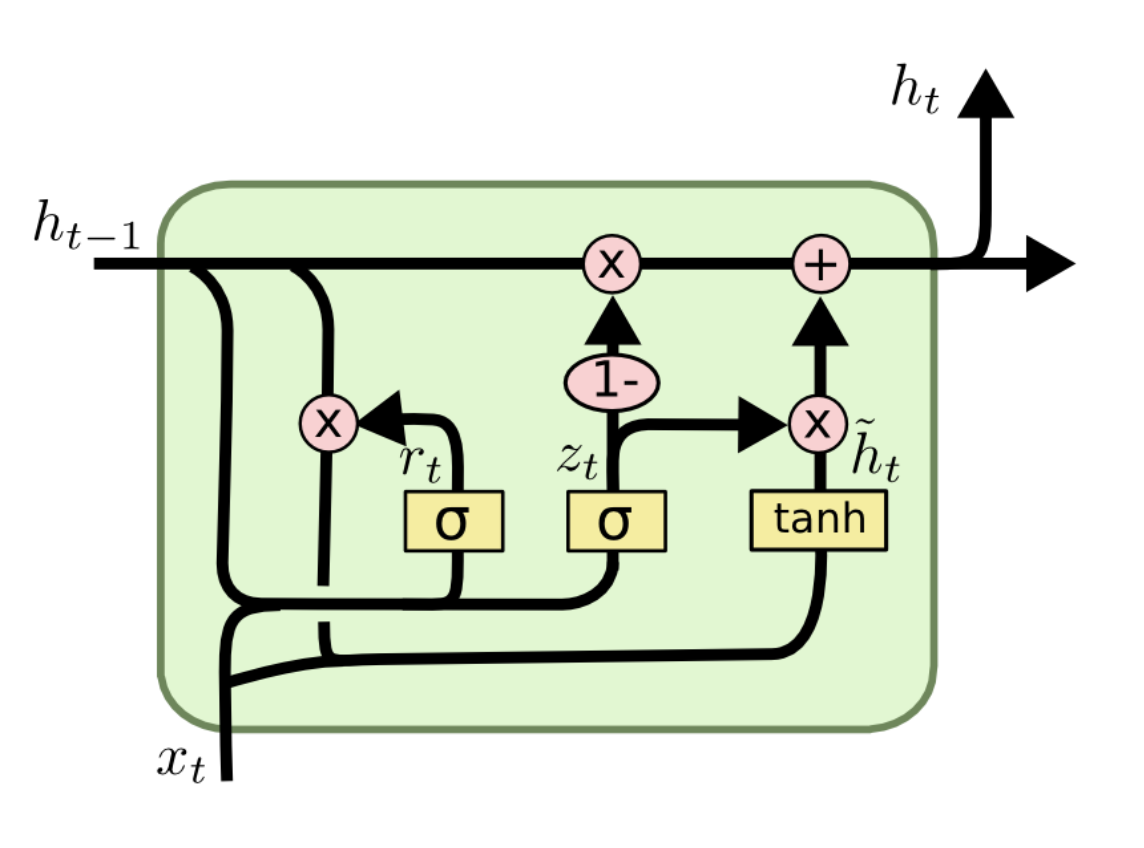
\includegraphics [scale=0.40,angle=360]{figures/gru.png}
\caption{Structure of a Gated Recurrent unit (source: \cite{olah})}
\label{fig:gru}
\end{figure}

\indent\newline 
In the update gate, $x_{t}$ is plugged into the network unit and multiplied by the weight $W_{z}$. $h_{t-1}$ holds previous information and is also multiplied by its weight $U_{z}$. Further, a sigmoid activation transforms the result into a value between 0 and 1 \cite{kosta}:

\indent\newline 
$z_{t} = \sigma(W_{z} x_{t} + U_{z} h_{t-1})$

\indent\newline 
Similar to the LSTM, in this step the GRU determines which parts of the past information to pass along in the structure, where a value of 1 means copying all of the past information and a value of 0 means keeping none of the information. Further, the reset gate is used to determine which parts of the information to forget. The same logic of the update gate applies to the reset gate:

\indent\newline 
$r_{t} = \sigma(W_{r} x_{t} + U_{r} h_{t-1})$

\indent\newline 
The next step of the process is introducing a memory content, in order for the network to be able to utilize the reset gate to store relevant information from the past \cite{kosta}:

\indent\newline 
$\tilde{h_{t}} = tanh(W_{x_{t}} + r_{t} * U_{h-1})$

\indent\newline 
The equation allows the model to determine what to remove from previous learned information, before applying the nonlinear activation function tanh, to transform the results into values between -1 and 1. The last step of the GRU is using the update gate to decide what information to collect from the current memory content $\tilde{h_{t}}$ and the previous steps $h_{t-1}$ \cite{kosta}. In order to do so, the model calculates $h_{t}$, which is a vector with information for the current unit and with a function of passing the information down in the network structure:

\indent\newline 
$h_{t} = z_{t} * h_{t-1} + (1 - z_{t}) * \tilde{h_{t}}$

\subsection{CNN}
Convolutional neural networks (CNNs) is a type of feedforward neural network commonly used for image recognition and object classification. The structure of a CNN can be compared to the neurons in the human brain, where individual neurons respond to stimuli in several Receptive Fields (parts of the visual field) that overlap each other to cover the entire visual area \cite{saha}.   

\indent\newline 
\begin{figure}[H]
\centering
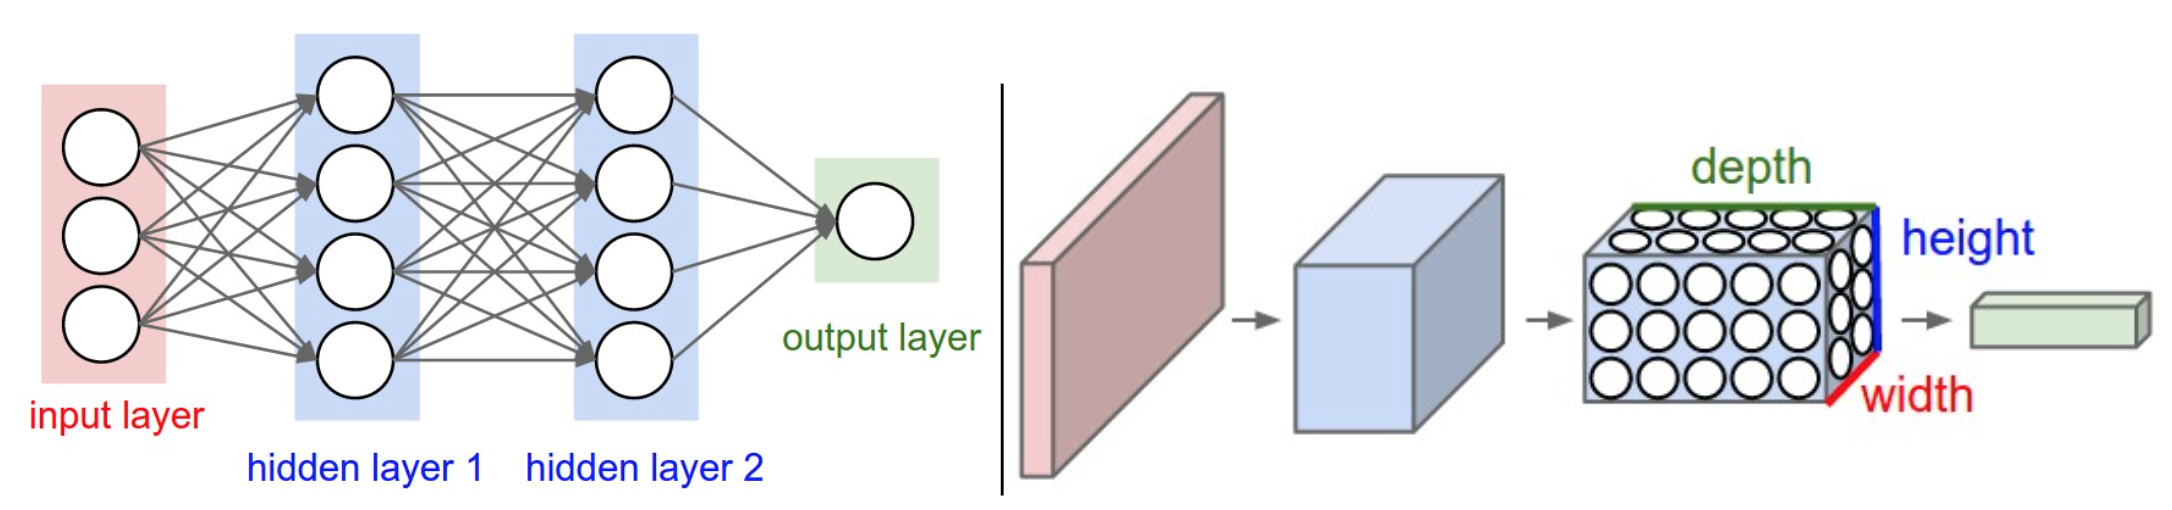
\includegraphics [scale=0.34,angle=360]{figures/cnn.png}
\caption{Structure of a CNN (source: \cite{zakka})}
\label{fig:cnn}
\end{figure}

\indent\newline 
The architecture of a CNN differs from standard neural networks in terms of making an assumption of input being images, which reduces the amount of parameters in the model. Figure 2.9 displays the difference between them where the neurons in a CNN are arranged in three dimensions, which consist of width, height and depth (illustrated in the third layer). The third dimension of depth refers only to an activation volume and not the depth of an entire neural network \cite{zakka}. In addition to having fully connected layers, as in standard neural networks, the CNN uses convolutional layers and pooling layers to reduce spatial size of the convolved feature. 

\indent\newline 
In the convolution layer a kernel K performs a matrix multiplication operation of K and P (the part of the image the kernel hovers over) equal to the number of stride lengths. The process is repeated until the image is traversed \cite{saha}. A CNN can have multiple convolutional layers, where the first one uses the input image to extract low-level features, while the last ones enables the model to adapt to the high-level features. Further, pooling layers reduce the amount of computational power needed to process the data, by reducing the spatial size of the convolved feature and by reducing dimensionality. There are two types of pooling, namely max pooling and average pooling, which consist of the model returning either the maximum value from the portion of the image covered by the kernel, or the average of all the values\cite{saha}. This is useful for extracting dominant features, as well as suppressing noisy activations. The last steps of the CNN-architecture consist of flattening the final output, before feeding it into a neural network (fully connected layer) to perform the classification.   

\section{Backtesting}
Developing new trading strategies can be a difficult task, and especially for investors to gain the confidence to implement the strategies in real-life trading. Backtesting, or systems testing, is an important method used by brokers and professional investors to test new strategies in a simulated environment. Backtesting reconstructs a trading scheme on historical data that would have occurred by using a particular trading strategy. An assumption within backtesting is that if a trading strategy has performed well in the past, it will also probably perform well in the future. Vice versa, if a trading strategy has performed poorly in the past, there is a good chance it will perform poorly in the future as well \cite{ni}.  To evaluate the performance of a trading strategy, several statistics and metrics can be used. This includes net profit or loss, volatility measures, average gain or loss, the percentage of capital exposed to the market, win-loss ratios, annualized return, and risk-adjusted return \cite{kuepper}. 

\indent\newline
Backtesting trading strategies comes with several potential pitfalls that can cause a seemingly successful strategy to fail when applying it to real-life trading: 

\begin{itemize}
\item \textbf{Market trend:} The time period and broad market trend are important factors to consider when conducting backtesting. If a strategy is backtested on a time period characterized by a consecutive bull market, the chances are the strategy will not perform well in a bear market. Backtesting should therefore be carried out on historical data with market conditions that include both a positive and negative market sentiment. 
\item \textbf{Universe:} Backtesting should also consider the universe the system is tested in. Developing a trading strategy targeted towards small cap stocks, and backtesting it in a universe of large cap stocks, will probably not translate into developing a successful strategy. It is therefore important to be aware of the limitations of a given strategy, while making sure the backtesting complies with these limitations.
\item \textbf{Volatility:} Traders who have leveraged accounts should focus their attention on volatility. Leveraged investors are subjected to margin calls, which occurs when an investor’s account value drops below the broker’s threshold. It is recommended for these investors to include volatility measures where the backtesting results in low volatility to minimize risk.   
\item \textbf{Risk:} Risk: A common mistake when backtesting is only focusing on annualized returns without taking into account the change in risk. Annualized returns is often used as a metric to compare the performance of a strategy against other suitable benchmark strategies. Risk-adjusted returns is an alternative metric which should be implemented in backtesting, in order to be certain that a potential trading strategy actually outperforms other benchmark strategies with an equal (or lower) level of risk.     
\item \textbf{Storytelling:} In situations where an investor has worked hard to develop a new trading strategy it is not uncommon to be biased. Since backtesting involves testing strategies on historical data (ex-post), it is possible that the investor justifies certain patterns and results with rationality that skews the results in the investor’s favour. This could potentially lead to applying strategies that underperform against other more well-established trading strategies. 
\item \textbf{Transaction costs:}  Simulating the transaction costs of each trade being made in backtesting is difficult because it would require the trades to be actually carried out under the       
\item \textbf{Transaction costs:} Simulating the transaction costs of each trade being made in backtesting is difficult because it would require the trades to be actually carried out in the real world. The bid-ask spread varies greatly between individual stocks, which can be hard to simulate correctly.        
\item \textbf{Over-optimization:} This is a condition where performance results are overfitted to the past. There is no guarantee the past will repeat itself, which means that fine-tuning parameters too much to the past can cause a strategy to fail in the present and future.    
\end{itemize}

\indent\newline   
Investors should keep these potential pitfalls in mind when backtesting a new trading strategy. Even if these frequent backtesting errors are avoided, it does not mean a good performance backtest will result in successful performance in the future. There will always be a chance of selection bias and a chance of history not repeating itself.   

\section{Transaction Costs}
As mentioned in the previous section, accurately simulating transaction costs is a common error when developing a trading strategy. To be able to accurately simulate the transaction cost for each given trade, it would require traveling back in time and actually executing each trade. To best cope with this problem, an investor needs to be aware of the different elements of transaction costs and how these elements affect the overall trading performance. The elements consist of:

\begin{itemize}
\item \textbf{Explicit transaction costs:} Broker commission and securities lending.
\item \textbf{Implicit transaction costs:} Arrival cost and implementation shortfall.
\end{itemize}  
\cite{morgan}

\indent\newline   
Explicit transaction costs can be decomposed into broker commissions and securities lending. Broker commissions is a fee an investor is required to pay in order to have a brokerage company facilitate a transaction. These fees vary between brokers, but it can have a substantial impact on returns, especially when a strategy requires frequent trading. Securities lending is directed at short selling activities. Short selling is when an investor borrows another investor's shares and sells these shares in the market, where the purpose is to buy back the same amount of shares at a later point at a lower price, before delivering the stocks back to the investor. Short sellers pay a borrowing fee to the investor who agreed to lend out the shares. 

\indent\newline   
Implicit transaction costs can be decomposed into arrival cost and implementation shortfall. Arrival cost is the difference between the arrival price and the execution price. The arrival price is the given price an asset is valued at the moment right before an order, while the execution price is the actual traded price \cite{morgan}. Implementation shortfall is the opportunity cost of placing an order below ask and when this order does not get executed. Placing an order below ask might lead to missing the opportunity of taking a position in a stock, which can affect portfolio composition and returns.This part of trading can be quite difficult, where an investor has to decide whether to avoid implementation shortfall all together by filling the current orders at ask, or placing an order below ask with hopes of getting a better entry price. 

\indent\newline   
A common way of backtesting deep learning trading algorithms is only including direct transactions costs. This underestimates the total transaction costs of a trading strategy, and can result in over-optimistic returns and results from the backtesting. Previous academic papers have usually assumed direct transaction costs of five basis points \cite{krauss}, while research carried out in 2009 on the Oslo Stock Exchange, showed arrival costs of 200 basis points by studying the period between 2000-2008 \cite{ode}. Since implicit transaction costs can potentially have a substantial impact on returns, it is important to include these costs in backtesting as an investor would experience arrival costs in practice.     

\section{Market Capitalization}
The market capitalization of a stock, also frequently mentioned as market cap, is the total market value of a company. It is a measure based on a company's worth in the open market and can be found by multiplying the number of outstanding shares with the last traded share price. How the open market determines a company's market cap is dependent on several factors. A common misconception is that it measures equity. The market evaluation of a company's total value is dependent on several factors. One of the most important factors is the company's ability to generate cash flow. This includes the ability of generating cash flow both in present time and in the future. The market expectation of a company's ability to generate future cash flow is one of the main reasons why a company sometimes can be either overvalued or undervalued. These situations of incorrect short-term evaluation create opportunities of possible profitable trades, which could potentially be exploited by deep learning algorithms.  

\subsection{Large Cap Stocks}
Stocks reviewed as large cap companies are big, solid companies with a stable positive cash flow, often associated with low risk. These stocks are referred to as blue chips, which originates from casinos where blue chips are the most valuable. Blue chips are often associated with solid earnings, low level of debt ratio and frequent cash dividends. Large cap stocks are often preferred by investors seeking a low level of risk, high volume of traded shares, and expectations of small fluctuations (low volatility) in share price. The Oslo Stock Exchange (OSE) is a smaller stock exchange which means that the classification of large cap stocks differ from larger stock exchanges such as S\&P 500, Dow Jones and Nasdaq in the US. These typically classify companies with a market capitalization of minimum 10 billion dollars as large cap stocks, while at the Oslo Stock Exchange this boundary is set to a market cap above 15 billion NOK (approximately 1.8 billion dollars). 

\subsection{Small Cap Stocks}
Companies regarded as small cap stocks are small, young companies, where a stable positive cash flow is not expected until several years down the line. The share prices tend to be more volatile with less liquidity than mature companies.These types of companies are often expected to experience significant growth in future years, which makes them difficult to evaluate. Because a positive net cash flow is not expected before many years, investing in these companies brings increased risk. Small caps are therefore often subject to speculations, where the share price can fluctuate greatly, based on changes in the company outlook and in periods of economic slowdowns. The stock exchanges in the US regard companies with a market cap below 2 billion dollars as small cap stocks, while the Oslo Stock Exchange regards companies with a market cap below 1 billion NOK (approximately 120 million dollars) as small cap stocks.   

\indent\newline   
Comparing historical returns favours investing in small caps stocks over large cap stocks. In the period from 1997 to 2012 the small cap index Russel 2000 had an annual return of 8.6\%, while the S\&P 500 had an annual return of 4.8\% \cite{segal}. On the other hand, the small cap index had one-third higher volatility compared to the S\&P 500. Comparing small cap funds with large cap funds in the period 2003-2013 showed a standard deviation (volatility measure) of 19.28 for small cap funds and 15.54 for large cap funds. A higher volatility translates into higher risk, which can make it difficult for investors, who have a limited number of stocks in their portfolio, to capitalize from investing in small cap stocks.  

\indent\newline   
Even though small cap stocks seem to outperform large cap stocks, they have higher volatility that translates into higher risk. Small cap investing with a portfolio consisting of a limited number of stocks can make it difficult for investors to capitalize from this type of investment strategy. 


\chapter{Data}
Market data on all stocks listed on the Oslo Stock Exchange as of 2021 are scraped from Yahoo Finance, using the Python library $\textit{yfinance}$ and each stock's unique ticker. This main data set is scraped using a max function in yfinance, which gives the maximum available historical data on each stock. The scraped data set provides data on daily dividend-adjusted closing share prices and daily traded volume for each stock. Further, market capitalization data is downloaded from Oslo Børs, which includes each stock's market capitalization at the end of the year in the period from 2003 until 2020. This is later used for separating small cap stocks from large cap stocks, and ultimately creating two different data sets based on a market cap threshold. Additional independent variables such as the VIX, Brent oil price, 10-year US treasury rate, and the USD/NOK foreign exchange rate are scraped individually from Yahoo Finance, where they are later merged with the two data sets. 

\section{Small Cap}
\begin{figure}[H]
\centering
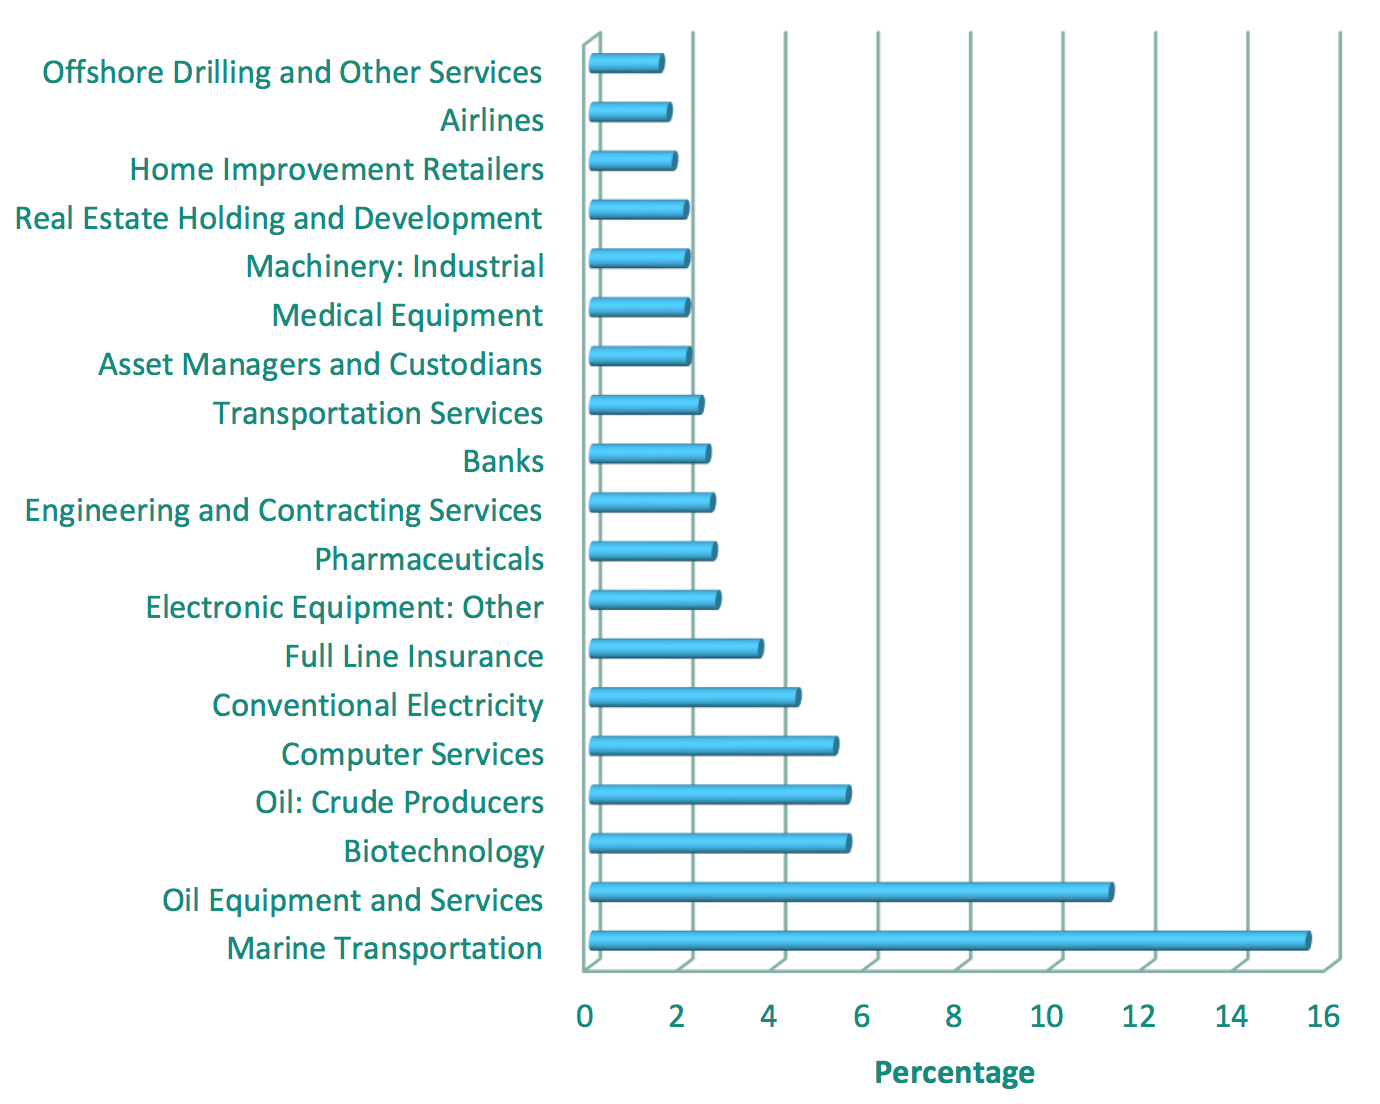
\includegraphics [scale=0.44,angle=360]{figures/smallsector.png}
\caption{OSESX Sector Allocation \cite{euronext}}
\label{fig:smallsector}
\end{figure}
\indent\newline 
Figure 3.1 shows the sector allocation of the small cap index as of 2021. The Index is dominated by marine transportation- and oil equipment and services companies, which accounts for approximately 25\% of the total index market cap. The smallest sectors consist of offshore drilling and airlines, and accounts for less than 2\% respectively of the total market cap. 

\indent\newline 
\begin{table}[ht]
\centering
\resizebox{\textwidth}{!}{\begin{tabular}{l|l}
\toprule
\textbf{Small cap statistics 2012-2020} \\ \midrule
Total number of stocks & 114 \\
Highest market capitalization & DOF Subsea (NOK 2,998,386,000 - 2012) \\
Lowest market capitalization & SeaBird Exploration (NOK 16,087,000 - 2017) \\
OSESX annualized returns  & 8.2\% \\ \bottomrule
\end{tabular}}
\caption{Small cap summary statistics}
\end{table}

\section{Large Cap}
\begin{figure}[H]
\centering
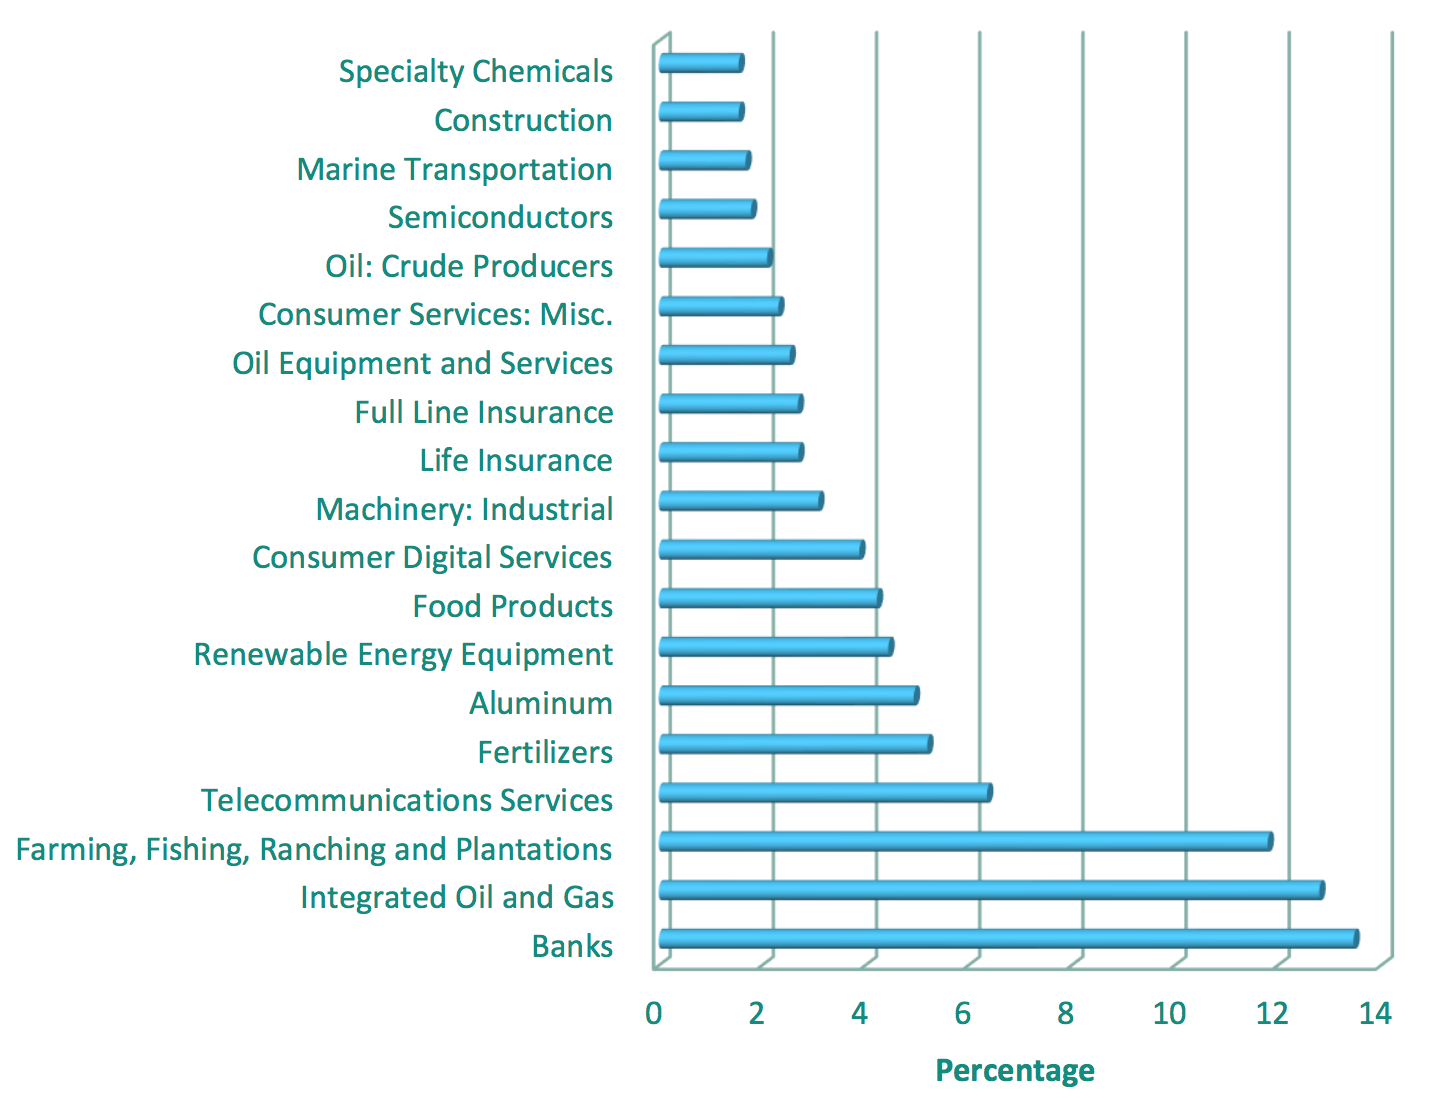
\includegraphics [scale=0.44,angle=360]{figures/largesector.png}
\caption{OSEBX Sector Allocation \cite{bors}}
\label{fig:largesector}
\end{figure}
\indent\newline 
Figure 3.2 illustrates the current sector allocation of the OSEBX index, mainly consisting of large cap stocks. The top three sectors are banks, integrated oil and gas, and farming, fishing, ranching and plantations, which represent approximately 38\% of the index total market cap. The bottom three sectors are specialty chemicals, construction, and marine transportation, where each sector makes up less than 2\% of the index. 

\indent\newline 
\begin{table}[ht]
\centering
\resizebox{\textwidth}{!}{\begin{tabular}{l|l}
\toprule
\textbf{Large cap statistics 2012-2020}  \\ \midrule
Total number of stocks & 64 \\
Highest market capitalization & Equinor (NOK 613,478,999,000 - 2018)  \\
Lowest market capitalization & Fjordkraft Holding (NOK 6,060,781,000 - 2019) \\
OSEBX annualized returns  & 16.7\% \\ \bottomrule
\end{tabular}}
\caption{Large cap summary statistics}
\end{table} 

\section{Software and Hardware}  
Data collection, data preparation and model development is conducted in Python 3.9, using Visual Studio as an integrated development environment (IDE). The models are developed with the library TensorFlow and with packages Keras and Scikit-learn. The deep learning models require a high level of computing power intensity, and to overcome this issue, they are trained and tested on GPU's provided by Google Cloud Platform.  

\chapter{Methodology}
The following chapter elaborates on the methods and techniques used to compare the returns of applying deep learning algorithms to small cap- and large cap stock predictions. It presents a variety of deep learning models used for predicting returns for both large cap and small cap stocks on the Oslo Stock Exchange. The aim of the research is to evaluate if the excess returns of investing in small caps can be capitalized on, through deep learning algorithms being able to detect patterns and relationships within historical data and by making accurate predictions of the probability of future share price development. An important part of a research process is choosing the appropriate method and research design to correctly analyze information and data on the topic, as well as for others to be able to assess the reliability and validity of the paper. 

\indent\newline
The methodology and techniques used in this paper is inspired by the work of Krauss et al. and Lund et al. \cite{krauss} \cite{lund}. This means that a similar approach and framework for developing the algorithms and assessing the models' predictive performance is applied to predicting small cap stock returns and comparing them with large cap stock returns. In addition to exploring the models' applicability to small cap stock returns, the paper will add on previous work in terms of implementing a gated recurrent unit (GRU) and a convolutional neural network (CNN).   

\indent\newline
The methodology can be decomposed into six sections, where the first section starts by presenting how the networks are trained and tested. Section two first elaborates on the main independent variable included for explaining the variability of stock returns, before presenting the different independent features that are included, with the aim of improving model performance. The section also explains the procedure of creating the target output. Section three gives an overview of the selected models for predicting small- and large cap stock returns. Further, section four introduces metrics used for evaluating predictive performance and portfolio performance, while section five describes the different portfolio strategies that are incorporated, in order to simulate how the network predictions can be utilized for real-life trading. Lastly, section six gives an overview of the different hyperparameters and their respective values for each model.

\section{Training and Testing}
The process of training the algorithms starts by defining study periods based on the collected data set, which contains data from January 2nd 2012 to December 30th 2020. This involves splitting the data into training and test sets. The training sets have intervals of 750 trading days, while the test sets have intervals of 250 trading days. Given that stock markets are closed on the weekend and during holidays, 250 trading days translates into approximately 1 year of trading, while 750 trading days translates into approximately 3 years worth of trading. The training periods is where the networks learn the patterns within the data and adjusts parameters to increase predictive accuracy, while the trading sets (test sets) are used to make out-of-sample predictions. The study periods are divided into a total of 8 unique periods, where each period is set up as rolling blocks of 1000 days. This means that the first period of trading (testing) starts 750 days into the data set, where these first days are lost to training. Further, each study period begins 250 days after the previous one, to ensure that the trading periods are non-overlapping, which means testing the models' predictions on the same data is avoided \cite{krauss}. 
\indent\newline 
\begin{figure}[H]
\centering
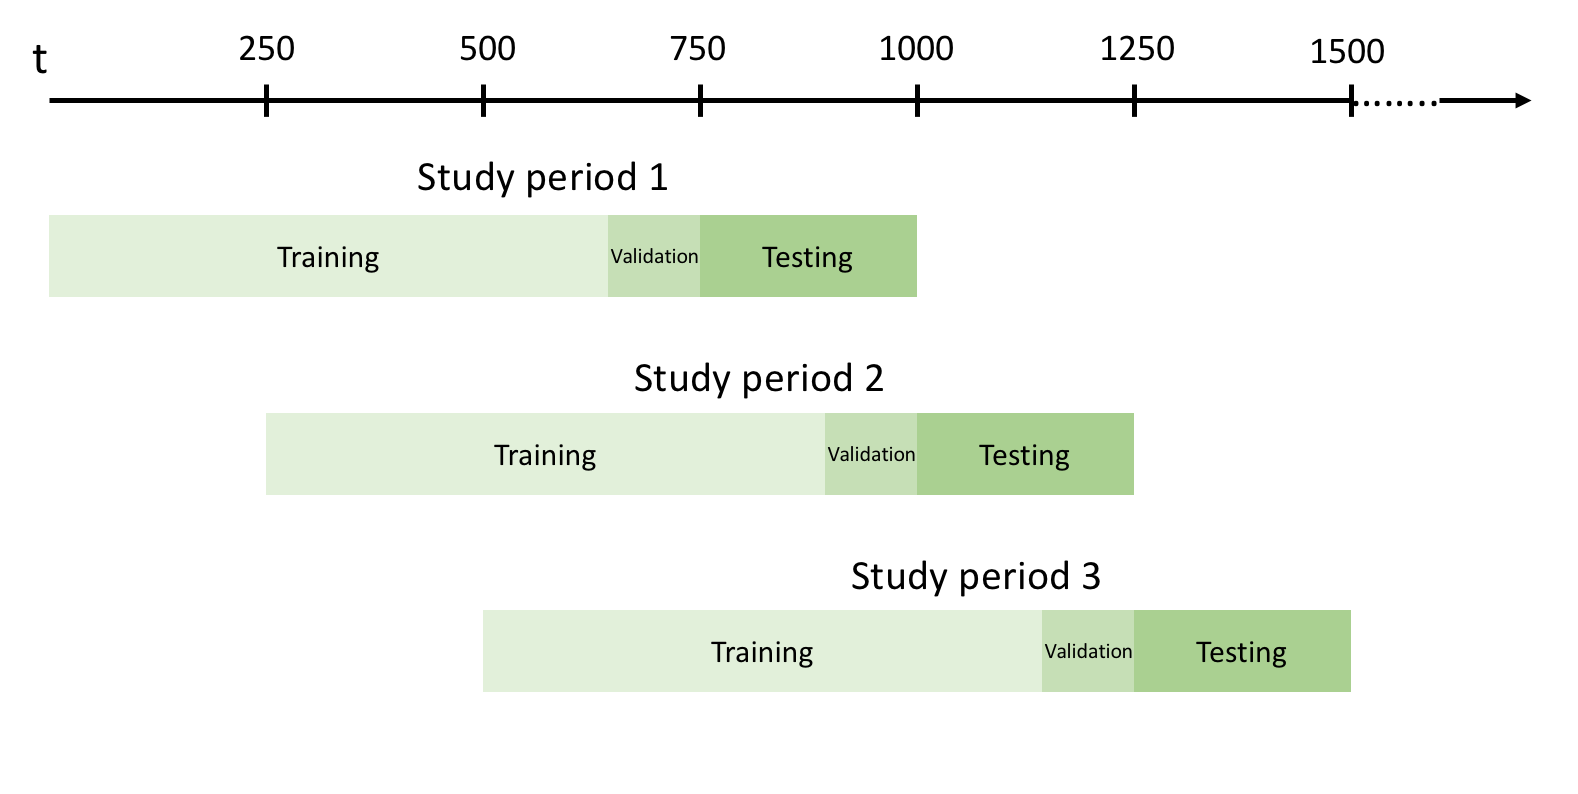
\includegraphics [scale=0.48,angle=360]{figures/study.png}
\caption{Rolling Study Periods}
\label{fig:study}
\end{figure}

\indent\newline 
Figure 4.1 illustrates the logical structure of the study periods, where the last 20\% of the training data is used for validation. Including validation sets is important in order to avoid selection bias related to the process of hyperparameters-optimization.

\indent\newline
The training and testing approach is applied to two different groups of stocks, where both groups are constituents on the Oslo Stock Exchange. The groups are constructed based on a market capitalization threshold updated at the end of each year. Small cap stocks are determined based on a market cap threshold equal to or below three billion NOK, while the threshold for large caps stocks is either equal to or above 6 billion NOK. It is difficult defining a definite threshold for what to characterize as a small cap stock and a large cap stock, but for the purpose of comparing returns between the two groups, a lower threshold is set for large cap stocks. This is a result of wanting to have a more balanced number of stocks in each group, as there are more small cap stocks listed on the Oslo Stock exchange compared to large cap stocks.  

\indent\newline
For both groups, $n_{i}$ denotes the number of stocks that are part of the groups at the last day in study period $\textit{i}$. Some of the stocks may not have a full data history for each training period, due to either being delisted or being listed at a later time. This also applies to stocks having a market cap changing above or below the thresholds during the study periods. If stocks do not exhibit share price data after a certain point in the trading period, they are included for trading up until this point. The same logic applies to stocks that are listed later than the starting point of the data, where these stocks are considered for trading after they have been listed.   

\section{Variables}
\subsection{Target Variable}
Following Krauss et al. the target variable $Y^{s}_{t + 1}$ represents a binary classification problem with two classes. The dependent variable for each stock $\textit{s}$ and date $\textit{t}$ is therefore equal to a value of either 1 or 0. This is determined on the basis of whether the one-period return $R^{1,s}_{t + 1}$ of stock $\textit{s}$ is larger or equal (class 1) to the cross-sectional median return of all stocks in period $\textit{t + 1}$, or smaller (class 0) than the cross-sectional median return. The classes are defined by ordering all one-period returns $R^{1,s}_{t + 1}$ of all stocks $\textit{s}$ in period $\textit{t + 1}$ in ascending order, and by putting them into two equally sized classes \cite{krauss}.  

\subsection{Independent Variables}
In order to improve model performance in terms of finding patterns and relationships within the data, several independent variables are used as input features for the models to train and test on. According to previous research, including a standardized one-day return with a sequence length of 240 days as a main independent variable seems to give good results with this type of neural network \cite{krauss}. To create the feature, the price process of stock $\textit{s}$ at time $\textit{t}$ is defined as $P^{s}$ = $(P^{s}_{t})_{t\in T}$ and where the simple return $R^{m,s}_{t}$ for a stock $\textit{s}$ over $\textit{m}$ periods is calculated in the following way:

\indent\newline
\begin{equation}
R^{m,s}_{t} = \frac{P^{s}_{t}}{P^{s}_{t-m}} - 1
\end{equation}

\indent\newline
The simple returns are calculated for each day and each stock $R^{1,s}_{t}$. Further, the mean and standard deviation are obtained from the training set. It is important to compute these measures only from the training set, as it ensures the network to avoid look-ahead biases. The mean $\mu^m_{train}$ is then subtracted from the simple returns and divided by the standard deviation $\sigma^{m}_{train}$ to standardize the returns:

\indent\newline
\begin{equation}
\tilde{R}^{m,s}_{t} = \frac{R^{m,s}_{t} - \mu^m_{train}}{\sigma^{m}_{train}}
\end{equation}

\indent\newline
The training process of an LSTM network requires input features to be divided into different sequences. As mentioned earlier, the standardized one-day returns $\tilde{R}^{1,s}_{t}$ have a sequence length of 240 days, which translates into approximately one year of trading. The standardized one-day returns are organized in overlapping sequences, where the feature vector is sorted by stocks $\textit{s}$ and date $\textit{t}$ in ascending order. To illustrate this, the first two sequences of the first stock $s_{1}$ have the form of $\lbrace\tilde{R}^{1,s_{1}}_{1}, \tilde{R}^{1,s_{1}}_{2}, ..., \tilde{R}^{1,s_{1}}_{240}\rbrace$ and $\lbrace\tilde{R}^{1,s_{1}}_{2}, \tilde{R}^{1,s_{1}}_{3}, ..., \tilde{R}^{1,s_{1}}_{241}\rbrace$ and so forth \cite{krauss}. 
   
\indent\newline
A large segment in the Norwegian economy is based on oil-related companies and represents a substantial part of the Oslo Stock Exchange's total market cap. Brent-crude price is therefore regarded as an important influence on the Oslo Stock Exchange and will be included as an input feature. Other independent variables that represent macroeconomic factors are the USD/NOK exchange rate and the 10-year US treasury rate, which are also included as input features. Additional input features are based on technical indicators and consist of the stock's daily volume, and moving averages with intervals of 50 and 200 days. Lastly, a measure of the broad market volatility is included as an input feature through daily data on the CBOE Volatility Index (VIX), also known as the fear index. The VIX captures market sentiment by measuring the relative strength of near-term price changes of the S\&P 500. It generates a 30-day forward projection of volatility, by being derived from prices of SPX index options with near-term expiration dates \cite{kuepper2021}.

\indent\newline
The reasoning behind including the 10-year US treasury rate and the VIX is their influence on small cap stocks. A majority of small cap stocks are not expected to generate positive cash flow before several years down the line. When investors calculate the net present value (NPV) of these companies, the rate of US treasuries affects the discount rate included in their NPV-analysis. 

\indent\newline
\begin{equation}
NPV = \sum_{t=1}^{n} \frac{R_{t}}{(1 + i)^{t}}
\end{equation}

\indent\newline
The equation above shows the formula for calculating the NPV, where $R_{t}$ is the expected net cash flow in a single time period $\textit{t}$, $\textit{i}$ is the discount rate which is based on potential returns from alternative investments, and $\textit{t}$ is the number of time periods. When investors decide on which discount rate to include in their analysis, they evaluate other returns from alternative investments. The 10-year treasury yield is a measure of a risk free rate and an alternative investment, and therefore affects the discount rate. E.g. if the risk free rate goes up, the discount rate also goes up and vice versa. A higher discount rate means that the present value of (especially) small cap stocks' future positive cash flow is negatively affected, since the positive cash flows are not expected until several years into the future. The 10-year US treasury rate should therefore, to a certain degree, explain the variability in small cap stocks' share price. Small cap stocks also tend to be more volatile than large cap stocks, which give reason to believe that the VIX could be a suitable input feature to include when predicting small cap stock returns. 

\section{Networks Variation}
The following models and network-variations are included with the aim of discovering the most suitable models for predicting small cap stock returns, in order to take advantage of the excess returns that comes with this group of stocks:

\indent \newline
\begin{itemize}
\item {\textbf{LSTM individual stocks:} The model is fed individual data for each stock which it trains on, before moving on to the next one. Input features only include the sequences of the last 240 stock returns.} 
\item {\textbf{LSTM all stocks:} The network trains on all stocks simultaneously with only one input feature, which consists of sequences of the last 240 stock returns. This network does not learn patterns and relationships within the data for each stock, but common relationships for all stocks.} 
\item {\textbf{LSTM stacked:} As apposed to the two previous, more basic models, this model has a network structure with two LSTM layers, which can potentially enable the network to discover deeper patterns within the data. The model trains on only the previous mentioned input feature.}
\item {\textbf{LSTM extra input features:} The last LSTM-variation follows the same principles as the LSTM trained on individual stocks, but it trains on data with additional input features. The reasoning behind including extra input features is to help the model explain the variability in stock returns.}
\end{itemize}

\section{Evaluation Metrics}
\subsection{Predictions}
Several threshold metrics for classification are used to assess and evaluate the accuracy of the networks. The section presents five performance metrics chosen on the basis of quantifying the prediction errors and accuracy of the networks, either by a fraction, ratio or rate. The first metric measures the networks' accuracy, which is the fraction of observations correctly classified:

\indent\newline
\begin{equation}
Accuracy = \frac{CP}{TP}
\end{equation}
\indent \newline 
\textit{Where,
\begin{itemize}
    \item[] $CP$ = Correct predictions
    \item[] $TP$ = Total predictions
\end{itemize}
}

\indent \newline 
The next metric is quite similar to the previous one, but instead of measuring the amount of correct predictions compared to total predictions, it compares the amount of positive/negative predictions with total positive/negative predictions:

\indent\newline
\begin{equation}
PA = \frac{CPP}{TPP}
\end{equation}
\indent \newline 
\textit{Where,
\begin{itemize}
	\item[] $PA$ = Positive accuracy
    \item[] $CPP$ = Correct positive predictions
    \item[] $TPP$ = Total positive predictions
\end{itemize}
}

\indent \newline 
Another metric incorporated to evaluate network performance is recall. The measurement looks at the ratio of the networks' correct positive prediction compared to the amount of actual positive observations:

\indent\newline
\begin{equation}
Recall = \frac{CPP}{TPO}
\end{equation}
\indent \newline 
\textit{Where,
\begin{itemize}
    \item[] $CPP$ = Correct positive predictions
    \item[] $TPO$ = Total positive observations
\end{itemize}
}

\indent \newline 
The next metric is the F-score. It uses the positive accuracy and recall to measure the networks' predictive accuracy in terms of robustness:

\indent\newline
\begin{equation}
F-Score = \frac{PA * Recall}{PA + Recall}
\end{equation}
\indent \newline 
\textit{Where,
\begin{itemize}
    \item[] $PA$ = Positive accuracy
\end{itemize}
}

\indent \newline 
The fifth and last evaluation metric is binary cross-entropy, which is the networks' loss function during training. In addition to measuring if predictions are correct or not, it also takes into account the difference between the predicted probabilities and actual outcomes \cite{lund}:

\indent \newline 
\begin{equation}
BCE = \frac{1}{N} \sum^{N}_{n=0} (y_{n}log[p_{n}] + (1 - y_{n})log[1 - p_{n}])
\end{equation}
\indent \newline 
\textit{Where,
\begin{itemize}
    \item[] $BCE$ = Binary cross entropy
    \item[] $N$ = Number of observations
    \item[] $y_{n}$ = Actual class of observation n
    \item[] $p_{n}$ = Predicted probability of observation n    
\end{itemize}
}

\subsection{Trading}
Multiple financial metrics are used for evaluating the trading performance of each network. These include annualized returns, standard deviation, Sharpe ratio, max drawdown, and value at risk (VaR). The chosen metrics capture both the returns from trading while also highlighting the risk associated with each model and strategy.

\indent \newline 
The Sharpe ratio is a measure which highlights the level of risk compared to returns. It is a ratio of average return earned in excess of the risk-free rate per unit of total risk or volatility \cite{fernando}. When analyzing the returns from trading in small caps and large caps, It is important to balance the results by not only comparing returns between the groups, but also the level of portfolio risk. Sharpe ratio is calculated in the following way:

\indent \newline
\begin{equation}
SR = \frac{R_{p} - R_{f}}{\sigma_{p}}
\end{equation}
\indent \newline 
\textit{Where,}
\indent \newline 
$SR$ = Sharpe ratio
\indent \newline 
$R_{p}$ = Return of portfolio
\indent \newline 
$R_{f}$ = Risk-free rate
\indent \newline 
$\sigma_{p}$ = Standard deviation of the portfolio's excess returns

\indent \newline 
Maximum drawdown is included to assess the portfolios' maximum observed loss from a peak to a trough, before attaining a new peak \cite{hayes}. In other words, it measures the greatest movement from a high point to a low point, which can interpreted as a representation of volatility and especially downside risk:

\indent \newline
\begin{equation}
MDD = \frac{TV - PV}{PV}
\end{equation}
\indent \newline 
\textit{Where,}
\indent \newline 
$MDD$ = Maximum drawdown
\indent \newline 
$TV$ = Trough value
\indent \newline 
$PV$ = Peak value

\indent \newline
Lastly, the value at risk (VaR) measures potential losses in a portfolio and their occurrence ratio. Volatility by itself is not a sufficient measure, as it does not differentiate between stocks with small fluctuations downwards in share price, but large fluctuations up in share price and vice versa. VaR addresses this issue by quantifying the risk of potential downside in a given stock. It is specifically directed towards the chance of experiencing big losses.  

\section{Strategies}
The models predict the probability $\widehat{\mathcal{P}}^{s}_{t+1|t}$ of a stock outperforming or underperforming the cross-sectional median return, where the models only use information up until time $\textit{t}$. For each period $\textit{t+1}$, the stocks are ranked in descending order based on their respective probability. The top of the ranking corresponds to the stocks the models evaluate as undervalued with expectations to outperform the cross-sectional median return, and is the basis for which stocks to buy. The bottom of the ranking corresponds to the stocks the models evaluate as overvalued with expectations of underperforming the cross-sectional median return, and dictates which stocks to short. This approach makes for several different portfolio strategies, where the models are instructed to buy (short) $\textit{K}$ stocks. The following portfolio strategies are selected:

\indent \newline
\begin{itemize}
\item {\textbf{Long-only portfolio:} The strategy involves being only long in $\textit{K}$ stocks. This means that shorting is not allowed. Two long-only portfolios are selected, where one is instructed to hold five stocks at any given time (K=5), and the other is instructed to hold ten stocks (K=10).} 
\item {\textbf{Long-short portfolio:} This strategy replicates a common portfolio for professional investors. The strategy allows for going both long and short. The models are instructed to create a portfolio consisting of being long five stocks and being short five stocks (2K, K=5) at any given point.}
\item {\textbf{Short-only portfolio:} The last strategy involves an unconventional trading approach, by only allowing for short-selling. The models create a portfolio of the most overvalued stocks (based on the probability of underperforming the cross-sectional median return) and are instructed to hold five short positions at any given time (K=5).}
\end{itemize}  

\indent \newline



\section{Hyperparameters}

\chapter{Results}
\section{Overview}
This chapter presents the resulting findings from training and testing the recurrent neural networks, and the results from applying the predictive models to the suggested portfolio strategies. The second section presents an analysis of predictive performance when applied to small cap and large cap stock returns. Section three presents an analysis on financial results from implementing the different portfolio strategies, where small cap portfolio performance is measured before transaction costs and compared with large cap portfolio performance. Portfolio performance after transaction costs is assessed on the basis of only including costs related to broker commissions in the backtesting. An assumption with backtesting the models is that portfolio positions are re-balanced during the closing auction call, which means that there is no need for including arrival costs related to the bid-ask spread. Lending fees for short-selling and implementation shortfall is not simulated. Lastly, small cap and large cap portfolio performance is compared with the returns of a diversified small cap portfolio and a diversified large cap portfolio, which are based on all stocks included in the data sets. This gives suitable reference measures to assess whether or not recurrent neural networks can be employed to predict small cap stock returns and if they can be used as a trading tool for consistently achieving excess returns. 

\subsection{Models}
The listed models below are the selected RNNs for predicting the probability of a stock outperforming the cross-sectional median return the next day (t+1). There are a total of 12 selected models from 6 different variations of RNNs, as a result of each network being applied to small cap and large cap stocks:

\indent \newline
\begin{itemize} 
\item {\textbf{lstm1\_small/large:} This is the network which trains on all stocks simultaneously, with only one input feature of the previous 240 stock returns.}  
\item {\textbf{lstm2\_small/large} This is the network which also trains on all stocks simultaneously, but an extra LSTM-layer is included in the network structure. It trains on only one input feature, which is the previous 240 stock returns.}
\item {\textbf{lstm3\_small/large:} The third LSTM-network trains on all stocks simultaneously, but with three LSTM-layers in the network structure. It trains on only one input feature, which is the previous 240 stock returns.}
\item {\textbf{lstmi8\_small/large:} The last LSTM-variation trains on all stocks simultaneously with additional input features of the VIX, brent-crude oil price, US 10-years treasury yield, USD/NOK exchange rate, and technical indicators consisting of 50- and 200-days moving averages.}
\item {\textbf{gru1\_small/large:} This is the GRU-network which trains on all stocks simultaneously, with one input feature of the previous 240 stock returns.}
\item {\textbf{grui8\_small/large:} This is the GRU-variation which trains on all stocks simultaneously with additional input features of the VIX, brent-crude oil price, US 10-years treasury yield, USD/NOK exchange rate, and technical indicators consisting of 50- and 200-days moving averages.}
\end{itemize}   

\subsection{Hyperparameters}
\begin{table}[ht]
\centering
\resizebox{\textwidth}{!}{\begin{tabular}{l|cccccc}
\toprule
 & lstm1\_small/large & lstm2\_small/large & lstm3\_small/large & lstmi8\_small/large & gru1\_small/large & grui8\_small/large \\ \midrule
Number of layers & 1 & 2 & 3 & 1 & 1 & 1 \\
Hidden units layer 1 & 50 & 50 & 50 & 50 & 50 & 50 \\
Hidden units layer 2 & - & 50 & 50 & - & - & - \\
Hidden units layer 3 & - & - & 50 & - & - & - \\
Output neurons & 1 & 1 & 1 & 1 & 1 & 1 \\
Activation function & Sigmoid & Sigmoid & Sigmoid & Sigmoid & Sigmoid & Sigmoid \\
Optimizer & RMSProp & RMSProp & RMSProp & RMSProp & RMSProp & RMSProp \\
Training steps & 2000 & 2000 & 2000 & 2000 & 2000 & 2000 \\
Batch size & 500 & 500 & 500 & 500 & 500 & 500 \\
Learning rate & 0.005 & 0.005 & 0.005 & 0.005 & 0.005 & 0.005 \\
Dropout & 0.1 & 0.1 & 0.1 & 0.1 & 0.1 & 0.1 \\ \bottomrule
\end{tabular}}
\caption{Hyperparameters}
\end{table}
\indent \newline
Table 5.1 shows the different hyperparameters incorporated in each of the RNNs. While comparing predictive performance between small caps and large caps is the main objective, and not optimizing model performance, hyperparameters-tuning has been carried out without achieving any significant changes to predictive performance. To reduce potential differences (and sources of error) when comparing predictive performance between small cap and large cap, the different hyperparameters are kept the same for each model.   
  
\section{Predictive Performance}
\begin{table}[ht]
\centering
\resizebox{\textwidth}{!}{\begin{tabular}{l|cccccc}
\toprule
 & \textbf{lstm1\_small} & \textbf{lstm2\_small} & \textbf{lstm3\_small} & \textbf{lstmi8\_small} & \textbf{gru1\_small} & \textbf{grui8\_small} \\ \midrule
Accuracy & 0.5829 & 0.5684 & 0.5637 & 0.5694 & \textbf{0.5840} & 0.5771  \\
Precision & 0.7572 & 0.6944 & 0.6781 & 0.7661 & \textbf{0.8726} & 0.7768  \\
Recall & \textbf{0.6144} & 0.6136 & 0.6125 & 0.6009 & 0.5974 & 0.6054  \\
F1-score & 0.6784 & 0.6515 & 0.6436 & 0.6735 & \textbf{0.7093} & 0.6805  \\
Binary cross-entropy & 0.687 & 0.755 & 0.794 & 0.765 & \textbf{0.664} & 0.689  \\ \bottomrule
\end{tabular}}
\caption{Predictive performance for small cap}
\end{table}

\begin{table}[ht]
\centering
\resizebox{\textwidth}{!}{\begin{tabular}{l|cccccc}
\toprule
 & \textbf{lstm1\_large} & \textbf{lstm2\_large} & \textbf{lstm3\_large} & \textbf{lstmi8\_large} & \textbf{gru1\_large} & \textbf{grui8\_large} \\ \midrule
Accuracy & 0.5037 & \textbf{0.5089} & 0.5071 & 0.5031 & 0.5081 & 0.5042  \\
Precision & 0.5485 & 0.5410 & 0.5636 & 0.6220 & 0.6227 &  \textbf{0.6649}  \\
Recall & 0.5116 & \textbf{0.5169} & 0.5145 & 0.5100 & 0.5139 & 0.5101  \\
F1-score & 0.5294 & 0.5286 & 0.5379 & 0.5605 & 0.5631 & \textbf{0.5773}  \\
Binary cross-entropy & 0.785 & 0.910 & 0.909 & 0.893 & \textbf{0.711} & 0.733  \\ \bottomrule
\end{tabular}}
\caption{Predictive performance for large cap}
\end{table}

\indent\newline
Tables 5.2 and 5.3 highlights predictive performance for the different models when predicting returns for small cap and large stocks. Table 5.1 shows that the overall best performing model for small cap is gru1\_small, scoring highest on accuracy, precision, F1-score and cross-entropy (lowest), while the lstm1\_small has the highest score on recall. For large cap stock returns, lstm2\_large barely outperforms the other models on measures of accuracy and recall. grui8\_large scores the highest on precision and F1-score, while gru1\_large has the best binary cross entropy score. It seems implementing additional layers in the network structure does not have any significant effect on predictive performance. This can be a result of the networks needing further fine-tuning of hyperparameters, or more observations for training. The additional input features also seems to have only a minor effect on model performance, which can be a result of previous returns reflecting all factors with an influence on share price.

\indent\newline
\begin{table}[ht]
\centering
\resizebox{10cm}{!}{\begin{tabular}{l|cccc}
\hline
 & \textbf{gru1\_small} & \textbf{grui8\_small} & \textbf{grui8\_large} & \textbf{gru1\_large} \\ \midrule
Accuracy & \textbf{0.5840} & 0.5771 & 0.5042 & 0.5081 \\
Precision & \textbf{0.8726} & 0.7768 & 0.6649 & 0.6227 \\
Recall & 0.5974 & \textbf{0.6054} & 0.5101 & 0.5139 \\
F1-score & \textbf{0.7093} & 0.6805 & 0.5773 & 0.5631 \\
Binary cross-entropy & \textbf{0.664} & 0.689 & 0.733 & 0.711 \\ \bottomrule
\end{tabular}}
\caption{Comparison of top performing models}
\end{table}

\indent\newline
\indent\newline
Table 5.4 illustrates the top two models for each group of stocks, based on equally weighting each performance measure. Comparing predictive performance across both group, shows that predictive models trained on small cap data outperforms models trained on large cap data on every performance measure. There are relatively big differences in all measures. The accuracy for the large cap models are just above 50\%, which is close to a random guess, while the two small cap models have accuracy measures of 58.4\% and 57.7\%, respectively. The binary cross entropy score is arguably the most important performance measure, as it accounts for how far the predicted probabilities are from the true values, and is the basis for which stocks to invest in. Also here, the small cap models outperform the large cap models with scores of 0.664 and 0.689, and 0.733 and 0.711 for the large cap models.     

\section{Portfolio Performance before Transaction Costs}
The following section presents the results from backtesting each model with a portfolio strategy consisting of only long-positions. The models instruct which five stocks to invest in each trading day, based on the predicted probability of a stock outperforming the cross-sectional median return the next day, and where all positions are weighted equally. Portfolio performance is assessed without taking into account transaction costs.    

\subsection{Small cap}
\begin{table}[ht]
\centering
\resizebox{\textwidth}{!}{\begin{tabular}{l|cccccc|c}
\toprule
Annualized & \textbf{lstm1\_small} & \textbf{lstm2\_small} & \textbf{lstm3\_small} & \textbf{lstmi8\_small} & \textbf{gru1\_small} & \textbf{grui8\_small} & {\color[HTML]{656565} \textbf{benchmark\_small}} \\ \midrule
Return & \textbf{1.1556} & 1.1023 & 0.8226 & 0.7030 & 0.6402 & 0.5194 & {\color[HTML]{656565} 0.1313} \\
Standard deviation & 0.3589 & 0.4120 & 0.3537 & 0.3768 & \textbf{0.3237} & 0.3320 & {\color[HTML]{656565} 0.1773} \\
Sharpe ratio & \textbf{3.1720} & 2.6341 & 2.2771 & 1.8202 & 1.9234 & 1.5128 & {\color[HTML]{656565} 0.6435} \\
Max drawdown & \textbf{0.2816} & 0.6022 & 0.6121 & 0.4382 & 0.5852 & 0.4265 & {\color[HTML]{656565} 0.6354} \\
VaR 5\% & \textbf{0.5653} & 0.4247 & 0.2409 & 0.0833 & 0.1075 & -0.0265 & {\color[HTML]{656565} -0.1602} \\ \bottomrule
\end{tabular}}
\caption{Small cap trading performance (long, K=5)}
\end{table}

\indent\newline
The table above shows the annualized performance metrics for each model when applied to a long-portfolio of five stocks. The portfolio termed benchmark\_small represents a diversified portfolio consisting of each small cap stock included in the data set, and is used as a benchmark measure. Analyzing the different metrics shows that the lstm1\_small network is the top-performing model with annualized returns of 115.56\%. Further, the model generates the highest Sharpe ratio, with a ratio of 3.17, as well as the best measure on value at risk. There is a 5\% probability of realizing an annualized return lower than 56.53\%, which is an exceptionally good annualized return. Taking into consideration the substantial annualized returns, a max drawdown of 28.16 percentage points indicates a moderate to low level of downside risk during the period (in addition to the VaR-measure). The lstm2\_small is the second best performing model, with an annualized return of 110.23\%. Even though this network nearly generates the same amount of annualized returns as lstm1\_small, the portfolio composition has a higher risk, illustrated by a Sharpe ratio of 2.63 and a standard deviation of 41.2\%. It also has a higher downside risk with a max drawdown of 60.22 percentage points.  

\indent\newline 
\begin{figure}[H]
\centering
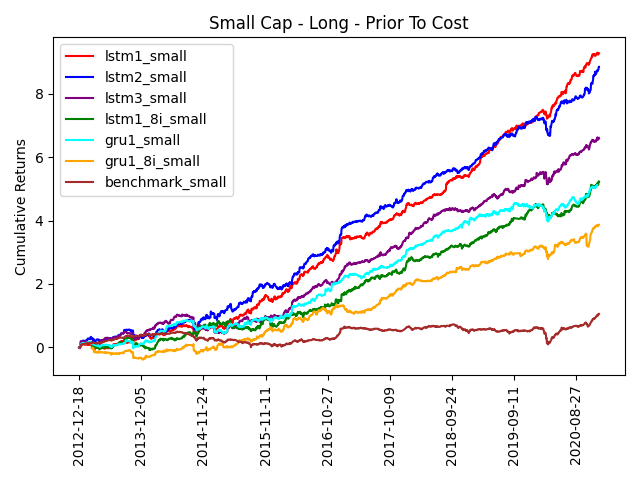
\includegraphics [scale=0.60,angle=360]{figures/cumulative_small_cap_return_no_cost.png}
\caption{Trading performance - small cap (long, K=5)}
\label{fig:smalltrading}
\end{figure}

\indent\newline 
Figure 5.1 further illustrates the findings with the two LSTM-models clearly outperforming the other models in terms of cumulative returns. The lstm1\_small generates cumulative returns of 928\%, while the worst-performing model grui8\_small generates cumulative returns of 386\%. All of the RNNs show promising results in terms of achieving excess returns, where the benchmark portfolio is outperformed with at least twice the cumulative returns, "only" generating cumulative returns of 105\%.  

\indent\newline 
An interesting part of the trading period is when the market crashed in the first half of 2020 during the breakout of the Corona-virus, and where the market cap of the Oslo Stock Exchange plummeted more than 30\% in the duration of approximately one month. While the graph illustrates each model experiencing a significant drop during the period, there is a big difference in drawdown between the top performing models. The drawdown of the lstm1\_small is relatively small considering the broad market drawdown, while the lstm2\_small experiences a much higher drawdown. This corresponds well with the lstm2\_small having higher risk, illustrated by a higher standard deviation and lower Sharpe ratio.    

\indent\newline
The analysis of predictive performance ranks gru1\_small and grui8\_small as the top-performing models for predicting small stock returns, while the analysis of portfolio performance ranks lstm1\_small and lstm2\_small as the most suitable models for achieving excess returns. A possible explanation for the differences in performance evaluation relates to the models' training process. The GRU-networks may have focused more on learning patterns within a larger number of stocks, enabling them to correctly classify a higher percentage of stocks outperforming the cross-sectional median return. The one- and two-layered LSTM may have learned patterns within a limited number of stocks that have been among the top-performing stocks during the period, enabling them to correctly predict high probabilities of the stocks that have performed well during the period. The LSTM-networks predictive performance may therefore have suffered from a higher rate of incorrect classifications, while still being able to generate higher returns.  

\subsection{Large cap}
\begin{table}[ht]
\centering
\resizebox{\textwidth}{!}{\begin{tabular}{l|cccccc|c}
\toprule
Annualized & \textbf{lstm1\_large} & \textbf{lstm2\_large} & \textbf{lstm3\_large} & \textbf{lstmi8\_large} & \textbf{gru1\_large} & \textbf{grui8\_large} & {\color[HTML]{656565} \textbf{benchmark\_large}} \\ \midrule
Return & 0.1576 & 0.1956 & 0.0805 & 0.1501 & 0.1911 & \textbf{0.2268} & {\color[HTML]{656565} 0.1539} \\
Standard deviation & 0.2733 & 0.2595 & \textbf{0.2443} & 0.2679 & 0.2616 & 0.2498 & {\color[HTML]{656565} 0.1782} \\
Sharpe ratio & 0.5135 & 0.6873 & 0.2590 & 0.4957 & 0.6648 & \textbf{0.8388} & {\color[HTML]{656565} 0.7670} \\
Max drawdown & 0.7419 & 0.8058 & \textbf{0.5564} & 0.5984 & 0.9088 & 0.8770 & {\color[HTML]{656565} 0.5535} \\
VaR 5\% & -0.2918 & -0.2311 & -0.3212 & -0.2906 & -0.2390 & \textbf{-0.1840} & {\color[HTML]{656565} -0.1391} \\ 
\bottomrule
\end{tabular}}
\caption{Large cap trading performance (long, K=5)}
\end{table}
\indent\newline 
Employing the selected RNNs to predicting large cap stock returns  results in much smaller differences between the models' portfolio performance, compared to the models employed to predicting small cap stock returns. Table 5.6 ranks grui8\_large as the best-performing model with an annualized return of 22.68\% and a Sharpe ratio of 0.84. It is also the top-performing model when assessing value at risk with a VaR of -18.4\%. On the other hand, it has one of the highest max drawdowns with a drawdown of 87.7 percentage points. The second best-performing model is lstm2\_large with an annualized return of almost 20\% and a Sharpe ratio of 0.69. It has a slightly lower max drawdown of 80 percentage points and -23\% VaR. lstm3\_large is the worst-performing RNN with annualized returns of 8\%, Sharpe ratio of 0.26, max drawdown of 55 percentage points and a VaR of -32\%. The model has the lowest fluctuation in annualized returns, illustrated by a standard deviation of 24\%.
\indent\newline 
\begin{figure}[H]
\centering
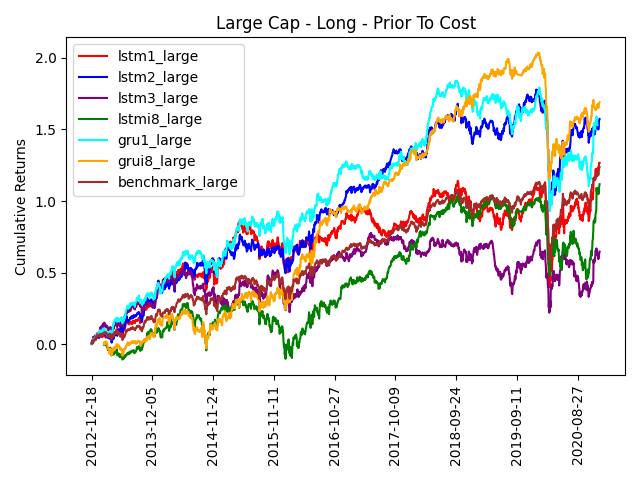
\includegraphics [scale=0.60,angle=360]{figures/cumulative_large_cap_return_no_cost.png}
\caption{Trading performance - large cap (long, K=5)}
\label{fig:largetrading}
\end{figure}
\indent\newline 
The graphical representation of cumulative returns further emphasizes the findings. Even though most of the RNNs outperform the large cap benchmark in terms of greater annualized returns, only grui8\_large is able to realize a higher Sharpe ratio than the benchmark portfolio. In other words, when adjusting for each portfolio's level of risk, the other models underperform against the benchmark. Comparing predictive performance and portfolio performance shows that the highest ranked RNNs (grui8\_large and gru1\_large) in terms of predictive performance are among the models that generates the highest annualized returns. This is more consistent than the models employed to predicting small cap stock returns.     

\subsection{Small cap vs large cap}
\begin{table}[ht]
\centering
\resizebox{\textwidth}{!}{\begin{tabular}{l|cccc|cc}
\toprule
Annualized & \textbf{lstm1\_small} & \textbf{lstm2\_small} & \textbf{grui8\_large} & \textbf{lstm2\_large} & {\color[HTML]{656565} \textbf{benchmark\_small}} & {\color[HTML]{656565} \textbf{benchmark\_large}} \\ \midrule
Return & \textbf{1.1556} & 1.1023 & 0.2268 & 0.1956 & 0.1313 & 0.1539 \\
Standard deviation & 0.3589 & 0.4120 & \textbf{0.2498} & 0.2595 & 0.1773 & 0.1782 \\
Sharpe ratio & \textbf{3.1720} & 2.6341 & 0.8388 & 0.6873 & 0.6435 & 0.7670 \\
Max drawdown & \textbf{0.2816} & 0.6022 & 0.8770 & 0.8058 & 0.6354 & 0.5535 \\
VaR 5\% & \textbf{0.5653} & 0.4247 & -0.1840 & -0.2311 & -0.1602 & -0.1391 \\ 
\bottomrule
\end{tabular}}
\caption{Comparing trading performance (long, K=5)}
\end{table}
\begin{table}[ht]
\centering
\resizebox{10cm}{!}{\begin{tabular}{l|cc|c}
\toprule
Annualized & \textbf{lstm1\_small} & \textbf{grui8\_large} & \textbf{Difference} \\ \midrule
Return & \textbf{1.1556} & 0.2268 & 0.9288 \\
Standard deviation & 0.3589 & \textbf{0.2498} & 0.1091 \\
Sharpe ratio & \textbf{3.1720} & 0.8388 & 2.3332 \\
Max drawdown & \textbf{0.2816} & 0.8770 & -0.5954 \\
VaR 5\% & \textbf{0.5653} & -0.1840 & 0.7493 \\
\bottomrule
\end{tabular}}
\caption{Top performing model for small and large cap (long, K=5)}
\end{table}
\indent\newline 
Comparing portfolio performance of the top models for each group of stocks shows substantial differences in annualized returns and portfolio risk. The top performing small cap model lstm1\_small generates approximately 90\ percentage points more in annualized returns compared to the best large cap model grui8\_large. The small cap model also clearly outperforms the large cap model when adjusting for risk, represented by a 2.33 higher Sharpe ratio. There are significant differences between downside risk, where the lstm1\_small has a max drawdown of 28 percentage points and a 5\% probability of realizing annualized returns below 56.53\%. The corresponding measures for grui8\_large is 87.7 percentage points and -18.4\%. The small cap models have a higher standard deviation which points to higher fluctuations in returns, but this can be a result of having a much higher rate of increase in annualized returns. 

\indent\newline 
\begin{figure}[H]
\centering
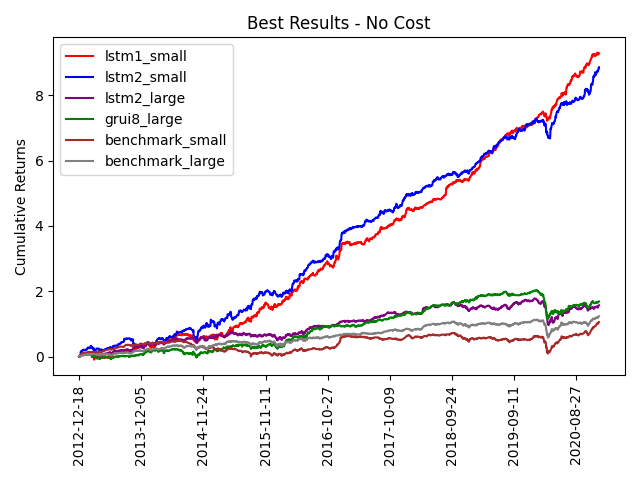
\includegraphics [scale=0.60,angle=360]{figures/cumulative_best_mix_cap_return_no_cost.png}
\caption{Small cap and large cap trading performance (long, K=5)}
\label{fig:mixtrading}
\end{figure}

\indent\newline 
Figure 5.3 shows a similar development in cumulative returns for both group of stocks during the first years of trading. In 2014 the small cap models' rate of returns starts to increase significantly more than the large cap models, while the large cap RNNs have a higher correlation with the benchmarks, resulting in a more similar development in cumulative returns throughout the period. Comparing benchmarks, shows that the small cap benchmark underperforms the large cap benchmark in the period. This should in theory be an advantage for the large cap models, as they are selecting stocks from a group with overall larger returns. A possible explanation to why the small cap models are able to outperform the large cap models, relates to the composition of the small cap group. There are often two types of companies that have a small market capitalization; young companies with expectations of experiencing a high rate of growth the coming years, and companies that are characterized by having high debt-to-equity ratios where several of them may be facing bankruptcy. This means there is a portion of small cap stocks with the potential to generate abnormal large returns, while the large cap models will not have these outperforming-stocks to choose from. When the small cap RNNs are able to differentiate between these two types of stocks, it leads to large differences in cumulative returns for the two groups of models employed to predicting stock returns. 

\indent\newline 
Having established that LSTM- and GRU-networks can be employed to predicting small cap stock returns, generate excess returns and outperform large cap stocks, the next section assess how the small cap models perform when transaction costs are included in the backtesting.

\section{Portfolio Performance after Transaction Costs}
This section implements explicit transactions costs in the form of broker commissions to evaluate the RNNs' portfolio performance in a more realistic trading environment. A fee of 3.5 basis points incurs each time a model chooses to buy or sell a stock. The commission fee is based on being a VIP-customer of Nordnet, which requires executing a minimum of 30 trades each month \cite{nordnet}. The models exceed this limit as the portfolios are re-balanced on a daily basis. 

\subsection{Small cap}
\begin{table}[ht]
\centering
\resizebox{\textwidth}{!}{\begin{tabular}{l|cccccc|c}
\toprule
Annualized & \textbf{lstm1\_small} & \textbf{lstm2\_small} & \textbf{lstm3\_small} & \textbf{lstmi8\_small} & \textbf{gru1\_small} & \textbf{grui8\_small} & {\color[HTML]{656565} \textbf{benchmark\_small}} \\ \midrule
Return & \textbf{0.7050} & 0.5595 & 0.2548 & 0.1379 & 0.1796 & -0.0535 & {\color[HTML]{656565} 0.1313} \\
Standard deviation & 0.3569 & 0.4107 & 0.3526 & 0.3760 & \textbf{0.3225} & 0.3309 & {\color[HTML]{656565} 0.1773} \\
Sharpe ratio & \textbf{1.9273} & 1.3204 & 0.6737 & 0.3208 & 0.5032 & -0.2141 & {\color[HTML]{656565} 0.6435} \\
Max drawdown & \textbf{0.3619} & 0.7544 & 0.9585 & 0.8874 & 1.0799 & 1.0187 & {\color[HTML]{656565} 0.6354} \\
VaR 5\% & \textbf{0.1180} & -0.1159 & -0.3250 & -0.4805 & -0.3510 & -0.5978 & {\color[HTML]{656565} -0.1602} \\
Total number of trades & \textbf{10,339} & 12,455 & 13,031 & 12,019 & 10,525 & 12,187 & {\color[HTML]{656565} -} \\ \bottomrule
\end{tabular}}
\caption{Small cap trading performance w/t.cost (long, K=5)}
\end{table}

\indent\newline 
Table 5.9 shows a significant (expected) drop in portfolio performance for the majority of the RNNs. The results from including transaction costs highlights the importance of models being able to identify stocks with a high probability of becoming future large cap stocks, and ultimately separate winners from losers. The lstm1\_small demonstrates a superior capability of identifying long-term winners compared to the lstm2\_small network. While the lstm2\_small model executes a total of 12,455 trades, the lstm1\_small only needs to perform 10,339 trades throughout the period. The ability of identifying winners translates into fewer trades, where winners are selected on the basis of a longer time frame, which has a large effect on portfolio performance.
\indent\newline 
\begin{figure}[H]
\centering
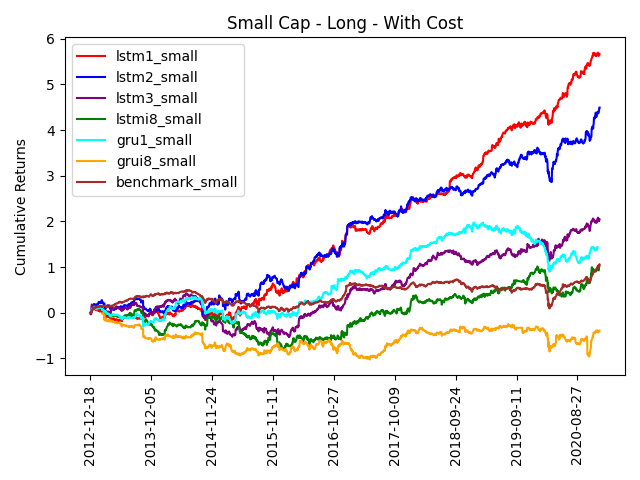
\includegraphics [scale=0.60,angle=360]{figures/cumulative_small_cap_return_with_cost.png}
\caption{Small cap trading performance w/t.cost (long, K=5)}
\label{fig:smallcost}
\end{figure}
\indent\newline 
Comparing the two top-performing models prior to transaction costs and after, highlights the impact transactions costs have on cumulative returns. Prior to transaction costs, there is only a small difference in total cumulative returns for the lstm1\_small and the lstm2\_small models (928\% vs 885\%), while after transaction costs the difference is much bigger (566\% vs 449\%). Despite the negative impact of transaction costs, every model is able to outperform the benchmark measure in terms of cumulative returns, except for the grui8\_small network. However, when adjusting for portfolio risk, only the one-layered and stacked LSTM-networks are able to outperform the benchmark, with Sharpe ratios of 1.92, 1.32 and 0.67.    

\subsection{Large cap}
\begin{table}[ht]
\centering
\resizebox{\textwidth}{!}{\begin{tabular}{l|cccccc|c}
\toprule
Annualized & \textbf{lstm1\_large} & \textbf{lstm2\_large} & \textbf{lstm3\_large} & \textbf{lstmi8\_large} & \textbf{gru1\_large} & \textbf{grui8\_large} & {\color[HTML]{656565} \textbf{benchmark\_large}} \\ \midrule
Return & -0.4671 & -0.4203 & -0.5497 & \textbf{-0.4163} & -0.4738 & -0.4706 & {\color[HTML]{656565} 0.1539} \\
Standard deviation & 0.2723 & 0.2588 & \textbf{0.2431} & 0.2676 & 0.2607 & 0.2489 & {\color[HTML]{656565} 0.1782} \\
Sharpe ratio & -1.7789 & -1.6907 & -2.3326 & \textbf{-1.6202} & -1.8837 & -1.9601 & {\color[HTML]{656565} 0.7670} \\
Max drawdown & 1.0000 & 1.0000 & 1.0000 & 1.0000 & 1.0000 & 1.0000 & {\color[HTML]{656565} 0.5535} \\
VaR 5\% & -0.9150 & \textbf{-0.8460} & -0.9496 & -0.8565 & -0.9026 & -0.8800 & {\color[HTML]{656565} -0.1391} \\
Total number of trades & 14,337 & 14,135 & 14,465 & \textbf{12,047} & 15,199 & 14,833 & {\color[HTML]{656565} -} \\ \bottomrule
\end{tabular}}
\caption{Large cap trading performance w/t.cost (long, K=5)}
\end{table}
\indent\newline 
Including transaction costs for the large cap models has an even larger negative impact on portfolio performance. None of the models are able to generate positive returns, and they are greatly outperformed by the benchmark portfolio. The least worst models are lstmi8\_large and lstm2\_large, with annualized returns of -41.63\% and -42.03\%, and Sharpe ratios of -1.62 and -1.69 respectively.  
\indent\newline 
\begin{figure}[H]
\centering
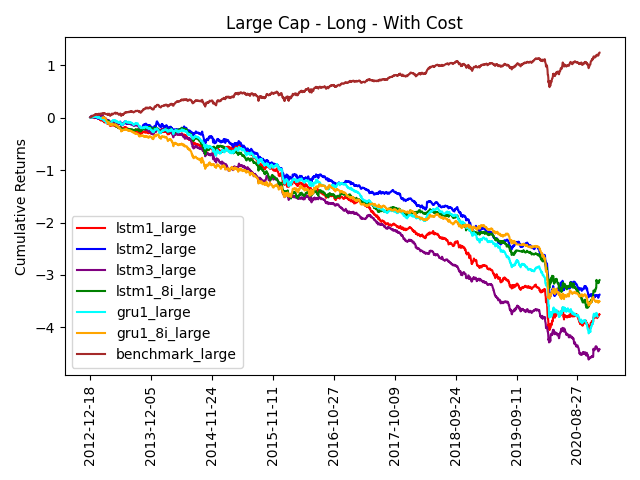
\includegraphics [scale=0.60,angle=360]{figures/cumulative_large_cap_return_with_cost.png}
\caption{Large cap trading performance w/t.cost (long, K=5)}
\label{fig:largecost}
\end{figure}
\indent\newline 
Figure 5.5 further emphasizes the findings, showing that the models' cumulative returns ranges from -309\% to -441\%, while the benchmark realizes cumulative returns of 123\%. In theory, it is not possible to generate negative returns below 100\% since the portfolio strategy consists of only being long and not short. However, the graph illustrates the resulting outcome if one were to keep adding investing capital to the portfolio throughout the period.    

\subsection{Small cap vs large cap}
\begin{table}[ht]
\centering
\resizebox{\textwidth}{!}{\begin{tabular}{l|cccc|cc}
\toprule
Annualized & \textbf{lstm1\_small} & \textbf{lstm2\_small} & \textbf{lstmi8\_large} & \textbf{lstm2\_large} & {\color[HTML]{656565} benchmark\_small} & {\color[HTML]{656565} benchmark\_large} \\ \midrule
Return & \textbf{0.7050} & 0.5595 & -0.4163 & -0.4203 & {\color[HTML]{656565} 0.1313} & {\color[HTML]{656565} 0.1539} \\
Standard deviation & 0.3569 & 0.4107 & 0.2676 & \textbf{0.2588} & {\color[HTML]{656565} 0.1773} & {\color[HTML]{656565} 0.1782} \\
Sharpe ratio & \textbf{1.9273} & 1.3204 & -1.6202 & -1.6907 & {\color[HTML]{656565} 0.6435} & {\color[HTML]{656565} 0.7670} \\
Max drawdown & \textbf{0.3619} & 0.7544 & 1.0000 & 1.0000 & {\color[HTML]{656565} 0.6354} & {\color[HTML]{656565} 0.5535} \\
VaR 5\% & \textbf{0.1180} & -0.1159 & -0.8565 & -0.8460 & {\color[HTML]{656565} -0.1602} & {\color[HTML]{656565} -0.1391} \\
Total number of trades & \textbf{10,339} & 12,455 & 12,047 & 14,135 & {\color[HTML]{656565} -} & {\color[HTML]{656565} -} \\ \bottomrule
\end{tabular}}
\caption{Comparison of trading performance w/t.costs (long, K=5)}
\end{table}

\indent\newline
\begin{table}[ht]
\centering
\resizebox{10cm}{!}{\begin{tabular}{l|cc|c}
\toprule
Annualized & \textbf{lstm1\_small} & \textbf{lstmi8\_large} & \textbf{Difference} \\ \midrule
Return & \textbf{0.7050} & -0.4163 & 1.1213 \\
Standard deviation & 0.3569 & \textbf{0.2676} & 0.0893 \\
Sharpe ratio & \textbf{1.9273} & -1.6202 & 3.5475 \\
Max drawdown & \textbf{0.3619} & 1.0000 & -0.6381 \\
VaR 5\% & \textbf{0.1180} & -0.8565 & 0.9745 \\
Total number of trades & \textbf{10,339} & 12,047 & -1,708 \\ \bottomrule
\end{tabular}}
\caption{Comparison of top models w/t.costs (long, K=5)}
\end{table}
\indent\newline
The tables above highlights how the small cap RNNs outperform the large cap models. Including explicit transaction costs further emphasize the vast differences in portfolio performance choosing to trade small cap stocks as apposed to large cap stocks. It is clear that employing RNNs to predict large stock returns is not a profitable trading strategy, where an investor would probably change his/hers investing strategy, rather than keep adding funds to an unsuccessful portfolio. The top-performing large cap models are able to outperform the benchmark without taking into consideration transaction costs, but when these are included they suffer from the high trading frequency.       
\indent\newline 
\begin{figure}[H]
\centering
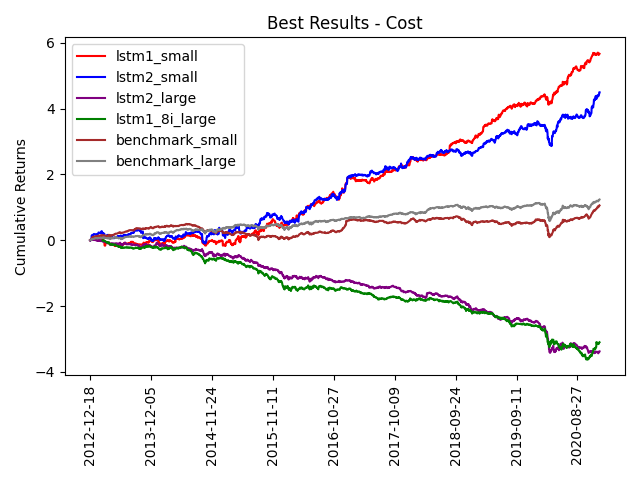
\includegraphics [scale=0.60,angle=360]{figures/cumulative_best_mix_cap_return_cost.png}
\caption{Comparison of trading performance w/t.cost (long, K=5)}
\label{fig:mixcost}
\end{figure} 
\indent\newline 
Figure 5.6 illustrates the superior performance of the small cap models. The small cap RNNs generate cumulative returns of 566\% and 449\%, while the large cap RNNs generate negative cumulative returns of 309\% and 337\%. When comparing the best-performing model for each group (lstm1\_small and lstmi8\_large) the small cap model outperforms the large cap model in terms of managing to achieve a 112 percentage points higher annualized return and a 3.54 higher Sharpe ratio. The lstm1\_small model also outperform the benchmarks, with a 1.28 higher Sharpe ratio than the benchmark\_small, and a 1.16 higher Sharpe ratio than the benchmark\_large. 

\indent\newline 
The resulting findings in this section suggest RNNs can be employed to predicting small cap stock returns for a long portfolio consisting of 5 stocks, re-balanced on a daily basis, and generate significant excess returns compared to large cap stocks. Evidence points towards the models having the ability to take advantage of the small cap stocks'  high volatility and fluctuation in share price as apposed to the lower volatility in large cap stocks.    

\indent\newline 
In the following sections, the models are tested with two additional portfolio strategies, namely a 50/50 long-short portfolio and a short-only portfolio.

\section{Additional Trading Strategies}
\subsection{Long-short 50/50 before transaction cost}
The long-short portfolio strategy consists of going long two stocks and going short two stocks, giving a total of four positions in the portfolio. As with the former strategy the portfolio is re-balanced each day, where long positions are based on the two highest predicted probabilities of a stock outperforming the cross-sectional median return, while short positions are based on the two lowest predicted probabilities.
\indent\newline 
\begin{table}[ht]
\centering
\resizebox{\textwidth}{!}{\begin{tabular}{l|cccccc|c}
\toprule
Annualized & \textbf{lstm1\_small} & \textbf{lstm2\_small} & \textbf{lstm3\_small} & \textbf{lstmi8\_small} & \textbf{gru1\_small} & \textbf{grui8\_small} & {\color[HTML]{656565} \textbf{benchmark\_small}} \\ \midrule
Return & \textbf{2.6358} & 2.0698 & 1.4935 & 1.1650 & 0.7671 & 0.3508 & {\color[HTML]{656565} 0.1313} \\
Standard deviation & 0.9795 & 1.0144 & 0.8187 & 0.9863 & \textbf{0.8777} & 1.4605 & {\color[HTML]{656565} 0.1773} \\
Sharpe ratio & \textbf{2.6732} & 2.0233 & 1.8030 & 1.1636 & 0.8543 & 0.2283 & {\color[HTML]{656565} 0.6435} \\
Max drawdown & \textbf{1.0132} & 1.0794 & 1.1876 & 1.6607 & 1.6244 & 3.5733 & {\color[HTML]{656565} 0.6354} \\
VaR 5\% & \textbf{1.0246} & 0.4012 & 0.1467 & -0.4573 & -0.6766 & -2.051 & {\color[HTML]{656565} -0.1602} \\ \bottomrule
\end{tabular}}
\caption{50/50 long-short small cap (2K, K=2)}
\end{table}
\indent\newline 
The lstm1\_small is the best-performing model, producing annualized returns of 263\% and a Sharpe ratio of 2.67. The annualized standard deviation is 97\% and there is a 5\% probability of realizing a return lower than 102\% (VaR). The worst-performing model is grui8\_small, with annualized returns of 35\% and a Sharpe ratio of 0.22. The big drop in returns for grui8\_small during the end of 2016 would require investing additional capital to the portfolio.  
\indent\newline 
\begin{figure}[H]
\centering
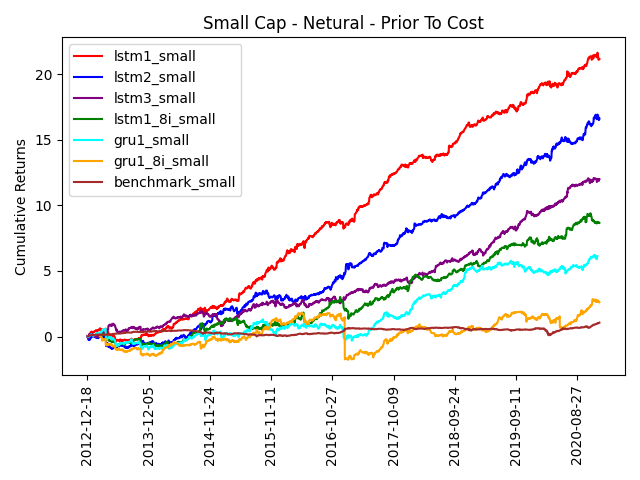
\includegraphics [scale=0.60,angle=360]{figures/cumulative_small_cap_return_no_cost_n.png}
\caption{Small cap trading performance 50/50 (2K, K=2)}
\label{fig:5050small}
\end{figure} 
\indent\newline 
The figure above displays each model realizing a higher cumulative return than the benchmark portfolio. All models outperform the benchmark in terms of having a higher Sharpe ratio, except for grui8\_small. 

\indent\newline 
\begin{table}[ht]
\centering
\resizebox{\textwidth}{!}{\begin{tabular}{l|cccccc|c}
\toprule
Annualized & \textbf{lstm1\_large} & \textbf{lstm2\_large} & \textbf{lstm3\_large} & \textbf{lstmi8\_large} & \textbf{gru1\_large} & \textbf{grui8\_large} & {\color[HTML]{656565} \textbf{benchmark\_large}} \\ \midrule
Return & -0.0884 & \textbf{0.2158} & -0.0514 & -0.1092 & -0.0762 & 0.1161 & {\color[HTML]{656565} 0.1539} \\
Standard deviation & 0.4402 & 0.3969 & \textbf{0.3795} & 0.4273 & 0.4983 & 0.3838 & {\color[HTML]{656565} 0.1782} \\
Sharpe ratio & -0.2401 & \textbf{0.5000} & -0.1809 & -0.2961 & -0.1876 & 0.2574 & {\color[HTML]{656565} 0.7670} \\
Max drawdown & 1.4138 & 1.2324 & 1.3844 & 1.3780 & 2.6298 & \textbf{0.8178} & {\color[HTML]{656565} 0.5535} \\
VaR 5\% & -0.8125 & \textbf{-0.4371} & -0.6757 & -0.8122 & -0.8959 & -0.5153 & {\color[HTML]{656565} -0.1391} \\ \bottomrule
\end{tabular}}
\caption{50/50 long-short large cap (2K, K=2)}
\end{table}
\indent\newline 
The top-performing model for the group of large cap stocks is lstm2\_large with annualized returns of 21.58\% and a Sharpe ratio of 0.50. The model has a lot more downside risk compared to the lstm1\_small represented by a 5\% probability of realizing a return lower than -43.71\%. lstmi8\_large is the worst-performing model with annualized returns of -10.92\% and a Sharpe ratio of -0.29.    
\indent\newline 
\begin{figure}[H]
\centering
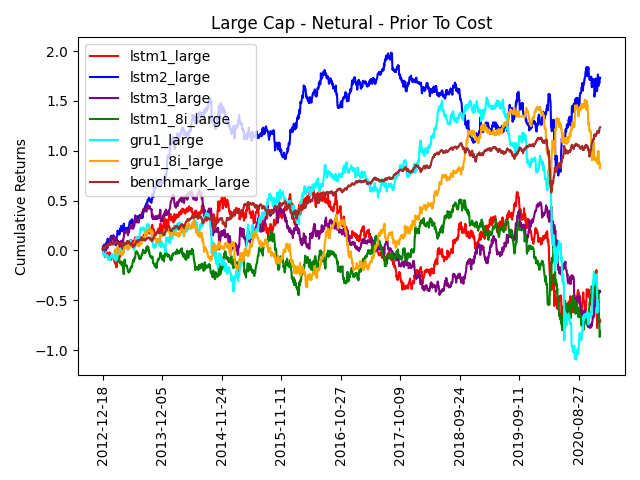
\includegraphics [scale=0.60,angle=360]{figures/cumulative_large_cap_return_no_cost_n.png}
\caption{Large cap trading performance 50/50 (2K, K=2)}
\label{fig:5050large}
\end{figure} 
\indent\newline 
The lstm2\_large is the only RNN which generates higher cumulative returns than the benchmark, but in terms of risk-adjusted returns (Sharpe ratio) none of the models are able to outperform the benchmark. Both of the GRU-networks generate higher cumulative returns than the benchmark during certain times of the trading period, but performance decline towards the end of the period.   

\indent\newline 
\begin{table}[ht]
\centering
\resizebox{10cm}{!}{\begin{tabular}{l|cc|c}
\toprule
Annualized & \textbf{lstm1\_small} & \textbf{lstm2\_large} & \textbf{Difference} \\ \midrule
Return & \textbf{2.6358} & 0.2158 & 2.4200 \\
Standard deviation & 0.9795 & \textbf{0.3969} & 0.5826 \\
Sharpe ratio & \textbf{2.6732} & 0.5000 & 2.1732 \\
Max drawdown & \textbf{1.0132} & 1.2324 & -0.2192 \\
VaR 5\% & \textbf{1.0246} & -0.4371 & 1.4617 \\ \bottomrule
\end{tabular}}
\caption{50/50 long-short comparison of top models (2K, K=2)}
\end{table}
\indent\newline 
A comparison of the top RNNs from each group of stocks shows extremely large differences in portfolio performance. The small cap LSTM-network generates 242 percentage points higher annualized returns and a 2.17 higher Sharpe ratio. There is also substantially less downside risk in the small cap portfolio, illustrated by a VaR of 102\% compared to a VaR of -43\%.

\indent\newline 
\begin{figure}[H]
\centering
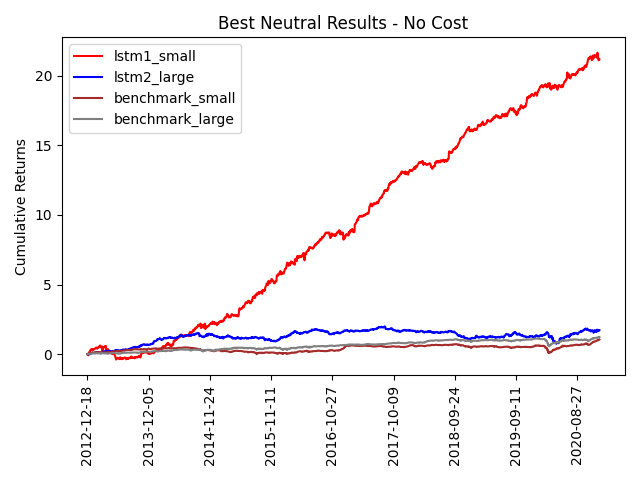
\includegraphics [scale=0.60,angle=360]{figures/cumulative_best_neutral_mix_return_no_cost.png}
\caption{Comparison of trading performance 50/50 long-short (2K, K=2)}
\label{fig:mix50}
\end{figure}

\subsection{Long-short 50/50 after transaction cost}
This section implements broker commission in order to simulate a more realistic trading environment. Fees for lending shares intended for short selling is not included in the backtesting. 
\indent\newline 
\begin{table}[ht]
\centering
\resizebox{\textwidth}{!}{\begin{tabular}{l|cccccc|c}
\toprule
Annualized & \textbf{lstm1\_small} & \textbf{lstm2\_small} & \textbf{lstm3\_small} & \textbf{lstmi8\_small} & \textbf{gru1\_small} & \textbf{grui8\_small} & {\color[HTML]{656565} \textbf{benchmark\_small}} \\ \midrule
Return & \textbf{2.1462} & 1.5309 & 0.9342 & 0.6613 & 0.2481 & -0.2203 & {\color[HTML]{656565} 0.1313} \\
Standard deviation & 0.9781 & 1.0131 & \textbf{0.8177} & 0.9855 & 0.8765 & 1.4598 & {\color[HTML]{656565} 0.1773} \\
Sharpe ratio & \textbf{2.1764} & 1.4940 & 1.1213 & 0.6534 & 0.2633 & -0.1627 & {\color[HTML]{656565} 0.6435} \\
Max drawdown & \textbf{1.1842} & 1.2057 & 1.3346 & 1.7118 & 2.6704 & 4.050 & {\color[HTML]{656565} 0.6354} \\
VaR 5\% & \textbf{0.5372} & -0.1355 & -0.4108 & -0.9597 & -1.1936 & -2.6216 & {\color[HTML]{656565} -0.1602} \\
Total number of trades & 11,236 & 12,366 & 12,836 & \textbf{10,714} & 11,864 & 12,148 & {\color[HTML]{656565} -} \\ \bottomrule
\end{tabular}}
\caption{50/50 long-short small cap w/t.cost (2K, K=2)}
\end{table}
\indent\newline 
Evaluating portfolio performance after including transaction costs shows that the lstm1\_small is the best performing model with annualized returns of 214\% and an annualized Sharpe ratio of 2.17. This means the costs related to broker commissions reduce the annualized returns with approximately 50 percentage points and the Sharpe ratio with 0.5. 
\indent\newline 
\begin{figure}[H]
\centering
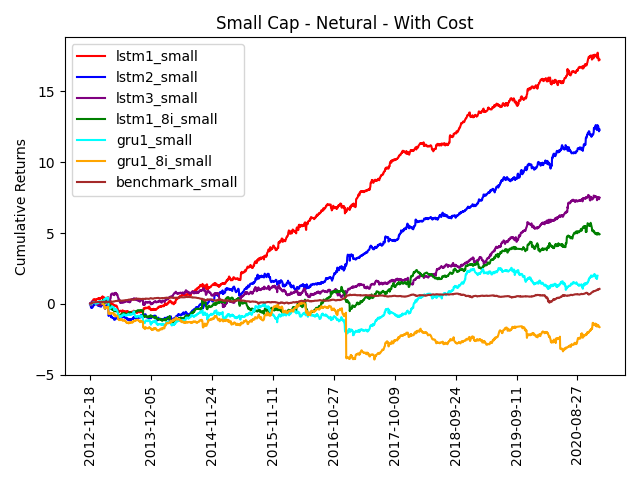
\includegraphics [scale=0.60,angle=360]{figures/cumulative_small_cap_return_with_cost_n.png}
\caption{Small cap trading performance w/t.cost 50/50 (2K, K=2)}
\label{fig:5050smallc}
\end{figure} 
\indent\newline 
All of the RNNs outperform the benchmark in terms of excess returns, except for grui8\_small. The GRU-network experiences a large drop in returns at the end of 2016, which it never recovers from. The two GRU-networks are the only models that are not able to outperform the benchmark when looking at Sharpe ratio.

\indent\newline 
\begin{table}[ht]
\centering
\resizebox{\textwidth}{!}{\begin{tabular}{l|cccccc|c}
\toprule
Annualized & \textbf{lstm1\_large} & \textbf{lstm2\_large} & \textbf{lstm3\_large} & \textbf{lstmi8\_large} & \textbf{gru1\_large} & \textbf{grui8\_large} & {\color[HTML]{656565} \textbf{benchmark\_large}} \\ \midrule
Return & -0.6427 & \textbf{-0.3538} & -0.6300 & -0.6250 & -0.6588 & -0.5042 & {\color[HTML]{656565} 0.1539} \\
Standard deviation & 0.4390 & 0.3965 & \textbf{0.3784} & 0.4266 & 0.4972 & 0.3836 & {\color[HTML]{656565} 0.1782} \\
Sharpe ratio & -1.5033 & \textbf{-0.9357} & -1.7107 & -1.5056 & -1.3597 & -1.3595 & {\color[HTML]{656565} 0.7670} \\
Max drawdown & 1.0000 & 1.0000 & 1.0000 & 1.0000 & 1.0000 & 1.0000 & {\color[HTML]{656565} 0.5535} \\
VaR 5\% & -1.3650 & \textbf{-1.0061} & -1.2525 & -1.3268 & -1.4767 & -1.1352 & {\color[HTML]{656565} -0.1391} \\
Total number of trades & 12,722 & 13,072 & 13,280 & \textbf{10,970} & 13,318 & 13,194 & {\color[HTML]{656565} -} \\ \bottomrule
\end{tabular}}
\caption{50/50 long-short large cap w/t.cost (2K, K=2)}
\end{table}
\indent\newline 
Assessing the large cap models after implementing broker commissions shows all of the models underperforming the benchmark. The lstm2\_large network is the least-worst performing model with annualized returns of -35\% and a Sharpe ratio of -0.93. The model with the lowest Sharpe ratio is lstm3\_large with a ratio of -1.71, while the model with lowest annualized returns is gru1\_large with returns of -65\%.  
\indent\newline 
\begin{figure}[H]
\centering
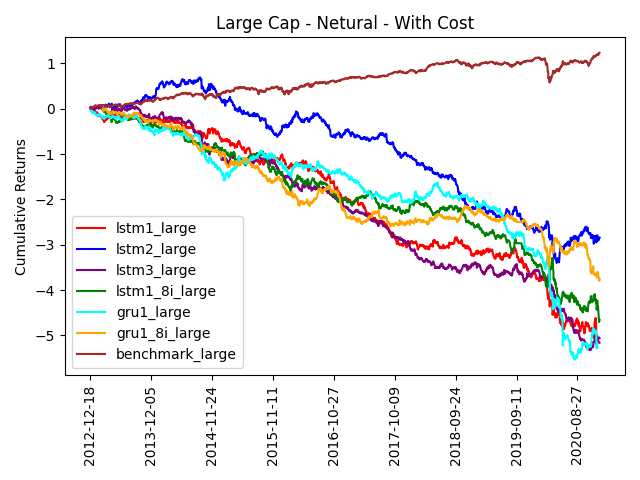
\includegraphics [scale=0.60,angle=360]{figures/cumulative_large_cap_return_with_cost_n.png}
\caption{Large cap trading performance w/t.cost 50/50 (2K, K=2)}
\label{fig:5050largec}
\end{figure} 
\indent\newline 
Figure 5.10 illustrates how all of the RNNs underperform the benchmark. The lstm2\_large outperforms the benchmark during a short period between 2013 and 2014, but quickly starts to decline after this period, ending with cumulative returns of -284\%.
\indent\newline 
\begin{table}[ht]
\centering
\resizebox{10cm}{!}{\begin{tabular}{l|cc|c}
\toprule
Annualized & \textbf{lstm1\_small} & \textbf{lstm2\_large} & \textbf{Difference} \\ \midrule
Return & \textbf{2.1462} & -0.3538 & 2.5000 \\
Standard deviation & 0.9781 & \textbf{0.3965} & 0.5816 \\
Sharpe ratio & \textbf{2.1764} & -0.9357 & 3.1121 \\
Max drawdown & \textbf{1.1842} & 4.0943 (1.00) & -2.9101 \\
VaR 5\% & \textbf{0.5372} & -1.0061 & 1.5433 \\
Total number of trades & \textbf{11,236} & 13,072 & -1,836 \\ \bottomrule
\end{tabular}}
\caption{Comparison top models 50/50 long w/t.cost (2K, K=2)}
\end{table}
\indent\newline 
Analyzing the top-performing model from each group of stocks highlights the massive differences in portfolio performance. The lstm1\_small RNN outperforms the lstm2\_large network in terms of generating 250 percentage points in excess annualized returns. When adjusting for risk, the large cap model is outperformed with a 3.11 higher Sharpe ratio. There is also considerably less downside risk, represented by a VaR of 53\% and -100\%. The small cap network also performs 1,836 trades less than the large cap model.  

\indent\newline 
\begin{figure}[H]
\centering
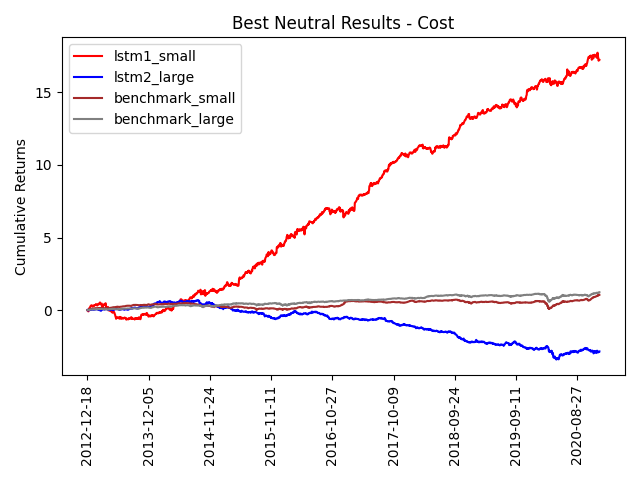
\includegraphics [scale=0.60,angle=360]{figures/cumulative_best_neutral_mix_return_cost.png}
\caption{Comparison of trading performance 50/50 long-short w/t.cost (2K, K=2)}
\label{fig:mix50c}
\end{figure}
\indent\newline 
The resulting findings suggest that the small cap models have an advantage by being able to choose from a group of stocks that have more extreme movements in returns. As discussed in section 5.3.3, when the small cap models learns the patterns and learns to differentiate between stocks that have a high probability of becoming short/long-term winners and short/long-term losers, they manage to capitalize on these extreme movements. The large cap models have less stocks to choose from with extreme movements in returns, which greatly affects performance when using a strategy that requires a high frequency of trading.

\subsection{Short-only before transaction costs}
This portfolio strategy consists of short-selling the five bottom ranked stocks, which is based on the models predicted probability of a stock outperforming the cross-sectional median return. The portfolio is re-balanced on a daily basis. The strategy does not account for potential complications regarding whether or not a stock is possible to short. 
\indent\newline     
\begin{table}[ht]
\centering
\resizebox{\textwidth}{!}{\begin{tabular}{l|cccccc|c}
\toprule
Annualized & \textbf{lstm1\_small} & \textbf{lstm2\_small} & \textbf{lstm3\_small} & \textbf{lstmi8\_small} & \textbf{gru1\_small} & \textbf{grui8\_small} & {\color[HTML]{656565} \textbf{benchmark\_small}} \\ \midrule
Return & 0.4804 & \textbf{0.4840} & 0.0641 & 0.2867 & 0.1453 & 0.3144 & {\color[HTML]{656565} 0.1313} \\
Standard deviation & 0.6716 & 0.4700 & 0.6196 & \textbf{0.4559} & 0.4762 & 0.6466 & {\color[HTML]{656565} 0.1773} \\
Sharpe ratio & 0.6895 & \textbf{0.9929} & 0.0755 & 0.5911 & 0.2687 & 0.4596 & {\color[HTML]{656565} 0.6435} \\
Max drawdown & 2.1090 & 1.3733 & 2.1498 & \textbf{0.8213} & 1.2765 & 1.5540 & {\color[HTML]{656565} 0.6354} \\
VaR 5\% & -0.6243 & \textbf{-0.2891} & -0.9550 & -0.4630 & -0.6380 & -0.7490 & {\color[HTML]{656565} -0.1602} \\ \bottomrule
\end{tabular}}
\caption{Small cap trading performance short-only (K=5)}
\end{table}
\indent\newline     
The lstm2\_small network is the top-performing model for the small cap RNNs. It realizes annualized returns of 48.4\% and a Sharpe ratio of 0.99. It also has less downside risk compared to the other models, illustrated by a max drawdown of 137 percentage points and a VaR of 28\%.
\indent\newline 
\begin{figure}[H]
\centering
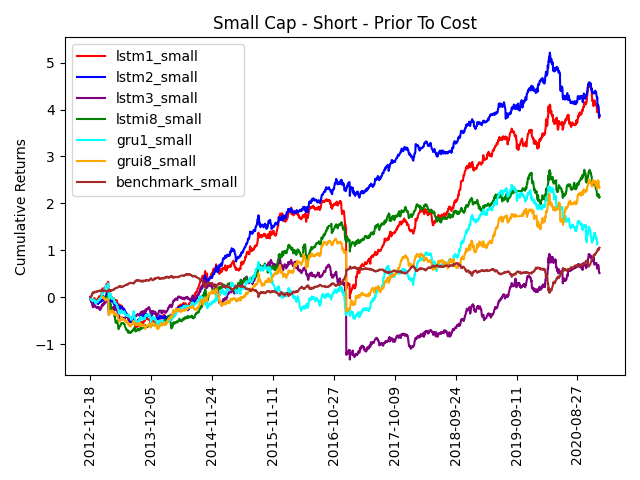
\includegraphics [scale=0.60,angle=360]{figures/cumulative_small_cap_return_no_cost_s.png}
\caption{Small cap trading performance short-only (K=5)}
\label{fig:shortsmall}
\end{figure} 
\indent\newline 
Comparing the networks with the benchmark shows each model being able to generate higher cumulative returns, except for the three-layered LSTM. However, when adjusting for risk, only the one- and two-layered LSTMs outperform the benchmark with higher Sharpe ratios.

\indent\newline 
\begin{table}[ht]
\centering
\resizebox{\textwidth}{!}{\begin{tabular}{l|cccccc|c}
\toprule
Annualized & \textbf{lstm1\_large} & \textbf{lstm2\_large} & \textbf{lstm3\_large} & \textbf{lstmi8\_large} & \textbf{gru1\_large} & \textbf{grui8\_large} & {\color[HTML]{656565} \textbf{benchmark\_large}} \\ \midrule
Return & -0.1142 & \textbf{-0.0300} & -0.0909 & -0.2030 & -0.1361 & -0.0946 & {\color[HTML]{656565} 0.1539} \\
Standard deviation & 0.2864 & 0.2730 & 0.2512 & 0.2786 & 0.2996 & \textbf{0.2429} & {\color[HTML]{656565} 0.1782} \\
Sharpe ratio & -0.4592 & \textbf{-0.1734} & -0.4308 & -0.7906 & -0.5121 & -0.4608 & {\color[HTML]{656565} 0.7670} \\
Max drawdown & 1.2328 & 0.8928 & 0.8715 & 1.6070 & 1.2907 & \textbf{0.8080} & {\color[HTML]{656565} 0.5535} \\
VaR 5\% & -0.5854 & \textbf{-0.4791} & -0.5043 & -0.6614 & -0.6289 & -0.4942 & {\color[HTML]{656565} -0.1391} \\ \bottomrule
\end{tabular}}
\caption{Large cap trading performance short-only (K=5)}
\end{table}
\indent\newline 
An analysis of the large cap models highlights lstm2\_large as the network with the least-worst performance results. The RNN generates negative annualized returns of 3\% and has a Sharpe ratio of -0.17. A closer look at table 5.20 shows that none of the large cap models are able to realize higher returns or Sharpe ratios than the benchmark.
 
\indent\newline 
\begin{figure}[H]
\centering
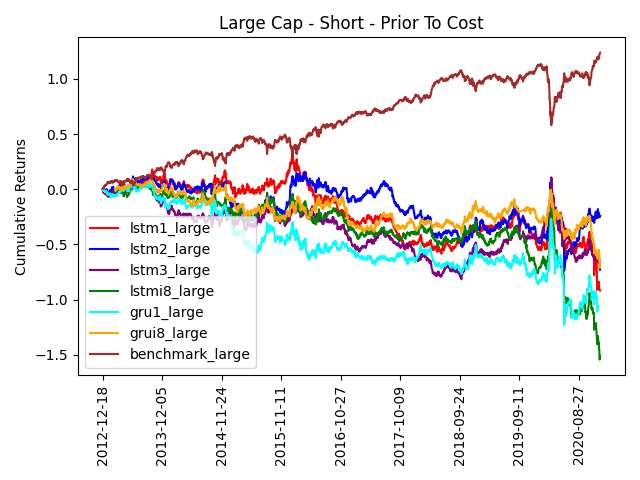
\includegraphics [scale=0.60,angle=360]{figures/cumulative_large_cap_return_no_cost_s.png}
\caption{Large cap trading performance short-only (K=5)}
\label{fig:shortlarge}
\end{figure} 
\indent\newline 
Similar to the small cap models the graph illustrates a negative correlation between the large cap RNNs and the benchmark. The reasoning behind this is that the trading strategy aims to capitalize on bearish market movements. This is especially visible during the market crash in 2020 with the break out of the Corona pandemic, where the benchmark returns drops with approximately 55 percentage points, while some of the RNNs' returns increase with approximately 40 percentage points.      
\indent\newline 
\begin{table}[ht]
\centering
\resizebox{10cm}{!}{\begin{tabular}{l|cc|c}
\toprule
Annualized & \textbf{lstm2\_small} & \textbf{lstm2\_large} & \textbf{Difference} \\ \midrule
Return & \textbf{0.4840} & -0.0300 & 0.5140 \\
Standard deviation & 0.4700 & \textbf{0.2730} & 0.1970 \\
Sharpe ratio & \textbf{0.9929} & -0.1734 & 1.1663 \\
Max drawdown & 1.3733 & \textbf{0.8928} & 0.4805 \\
VaR 5\% & \textbf{-0.2891} & -0.4791 & 0.1900 \\ \bottomrule
\end{tabular}}
\caption{Comparison of trading performance short-only (K=5)}
\end{table}
\indent\newline 
\begin{figure}[H]
\centering
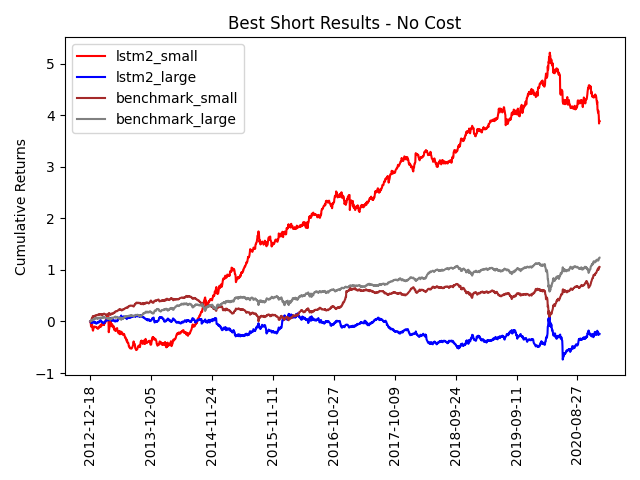
\includegraphics [scale=0.60,angle=360]{figures/cumulative_best_short_mix_return_no_cost.png}
\caption{Comparison of trading performance short-only (K=5)}
\label{fig:shortcomparison}
\end{figure} 
\indent\newline 
Assessing the best-performing model for each group of stocks prior to transaction costs shows how the small cap portfolio is able generate excess cumulative returns compared to the large cap portfolio and the benchmarks. The small cap portfolio has a 51 percentage points higher annualized return and a 1.16 higher Sharpe ratio than the large cap portfolio. The portfolio peaks during the market crash in 2020, where it capitalizes on the broad market fall. It seems the small cap model is able to profit from having the ability to learn patterns of a higher number of stocks within a long-term down trend and high volatility, compared to the large cap stocks that are more stable and have lower volatility.    

\subsection{Short-only after transaction costs}
This section presents an analysis on the short-portfolios where transaction costs are implemented for each trade. Lending rates for short-selling are not included in the backtesting. 
\indent\newline
\begin{table}[ht]
\centering
\resizebox{\textwidth}{!}{\begin{tabular}{l|cccccc|c}
\toprule
Annualized & \textbf{lstm1\_small} & \textbf{lstm2\_small} & \textbf{lstm3\_small} & \textbf{lstmi8\_small} & \textbf{gru1\_small} & \textbf{grui8\_small} & \textbf{benchmark\_small} \\ \midrule
Return & \textbf{-0.0944} & -0.1265 & -0.5823 & -0.2845 & -0.5210 & -0.3452 & 0.1313 \\
Standard deviation & 0.6705 & 0.4692 & 0.6186 & \textbf{0.4555} & 0.4747 & 0.6461 & 0.1773 \\
Sharpe ratio & \textbf{-0.1667} & -0.3065 & -0.9692 & -0.6625 & -1.1339 & -0.5611 & 0.6435 \\
Max drawdown & 2.4686 & \textbf{1.9144} & 4.6865 & 2.1632 & 4.3239 & 2.9465 & 0.3295 \\
VaR 5\% & -1.1973 & \textbf{-0.8983} & -1.6000 & -1.0339 & -1.3020 & -1.4080 & -0.1602 \\
Total number of trades & 13,193 & 14,011 & 14,835 & \textbf{12,151} & 15,231 & 14,031 & - \\ \bottomrule
\end{tabular}}
\caption{Small cap trading performance short-only w/t.cost (K=5)}
\end{table}
\indent\newline
Table 5.22 ranks lstm1\_small as the least-worst model when assessing annualized returns and returns adjusted for risk. It generates negative returns of 9.44\% and a negative Sharpe ratio of 0.16. Reviewing each model's performance suggest that the portfolio strategy does not show promising results, in light of none of the models being able to outperform the benchmark or generate positive returns.  
\indent\newline 
\begin{figure}[H]
\centering
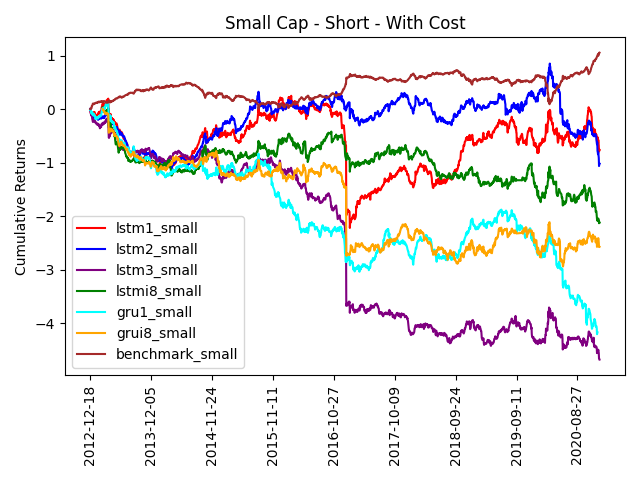
\includegraphics [scale=0.60,angle=360]{figures/cumulative_small_cap_return_with_cost_s.png}
\caption{Small cap trading performance short-only w/t.cost (K=5)}
\label{fig:shortlsmallc}
\end{figure} 
\indent\newline 
The lstm2\_small network outperforms the benchmark during a short period in 2020 (during the Corona market crash), but it experiences its highest drawdown right after, as the market quickly moves into another period characterized as a "bull-market". 

\indent\newline
\begin{table}[ht]
\centering
\resizebox{\textwidth}{!}{\begin{tabular}{l|cccccc|c}
\toprule
Annualized & \textbf{lstm1\_large} & \textbf{lstm2\_large} & \textbf{lstm3\_large} & \textbf{lstmi8\_large} & \textbf{gru1\_large} & \textbf{grui8\_large} & \textbf{benchmark\_large} \\ \midrule
Return & -0.7165 & \textbf{-0.6497} & -0.7351 & -0.7673 & -0.7779 & -0.7900 & 0.1539 \\
Standard deviation & 0.2855 & 0.2722 & 0.2509 & 0.2782 & 0.2989 & \textbf{0.2431} & 0.1782 \\
Sharpe ratio & -2.5699 & \textbf{-2.4498} & -2.9986 & -2.8201 & -2.6601 & -3.3205 & 0.7670 \\
Max drawdown & 5.7561 & \textbf{5.2951} & 5.9017 & 5.7403 & 6.2414 & 5.8861 & 0.0582 \\
VaR 5\% & -1.1862 & \textbf{-1.0975} & -1.1478 & -1.2250 & -1.2697 & -1.1900 & -0.1391 \\
Total number of trades & 13,821 & 14,219 & 14,781 & \textbf{12,001} & 14,669 & 14,789 & - \\ \bottomrule
\end{tabular}}
\caption{Large cap trading performance short-only w/t.cost (K=5)}
\end{table}
\indent\newline
The findings from analyzing the large cap models' performance when applied to a short-only portfolio shows extremely poor results. The different RNNs generate negative annualized returns between 60\% and 80\% and negative Sharpe ratios between 2.44 and 3.32. It would require regularly adding funds to the portfolios to be able to produce the results from the backtesting, as the models drop below 100\% in total cumulative returns.  
\indent\newline 
\begin{figure}[H]
\centering
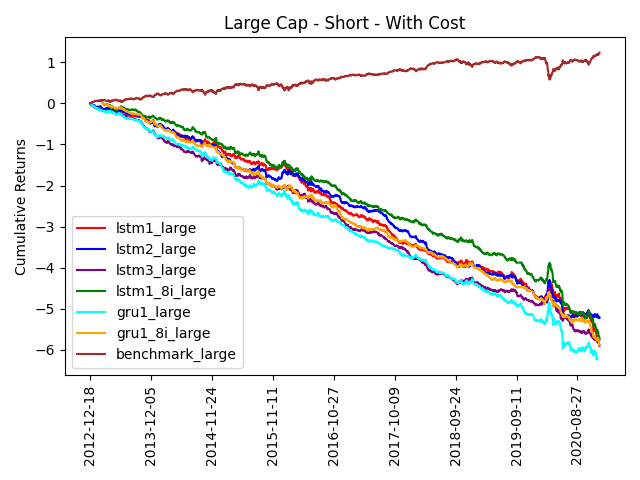
\includegraphics [scale=0.60,angle=360]{figures/cumulative_large_cap_return_with_cost_s.png}
\caption{Large cap trading performance short-only w/t.cost (K=5)}
\label{fig:shortlargec}
\end{figure} 
\indent\newline 
The figure above further illustrates the poor performance of the large cap models, where transaction costs increase the negative cumulative returns. The least-worst model (lstm2\_large) ends with cumulative returns of -521\%, while the worst model (gru1\_large) realizes cumulative returns of -622\%.

\indent\newline 
\begin{table}[ht]
\centering
\resizebox{10cm}{!}{\begin{tabular}{l|cc|c}
\toprule
Annualized & \textbf{lstm1\_small} & \textbf{lstm2\_large} & \textbf{Difference} \\ \midrule
Return & \textbf{-0.0944} & -0.6497 & 0.5553 \\
Standard deviation & 0.6705 & \textbf{0.2722} & 0.3983 \\
Sharpe ratio & \textbf{-0.1667} & -2.4498 & 2.2831 \\
Max drawdown & \textbf{2.4686} & 5.2951 & -2.8265 \\
VaR 5\% & \textbf{-1.1973} & -1.0975 & -0.0998 \\
Total number of trades & \textbf{13,193} & 14,219 & -1,026 \\ \bottomrule
\end{tabular}}
\caption{Comparison of trading performance short-only w/t.cost (K=5)}
\end{table}
\indent\newline 
\begin{figure}[H]
\centering
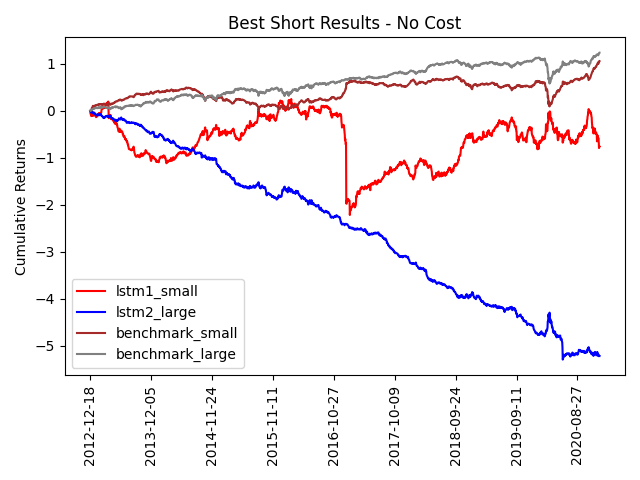
\includegraphics [scale=0.60,angle=360]{figures/cumulative_best_short_mix_return_cost.png}
\caption{Comparison of trading performance short-only w/t.cost (K=5)}
\label{fig:shortcomparisonc}
\end{figure} 
\indent\newline 
Analyzing the top-performing model for both small cap and large cap stocks after including transaction costs, reveals that the RNNs should not be employed to short-only portfolios. While neither model is able to generate positive returns, there are still significant differences in portfolio performance. The lstm1\_small generates a 55 percentage points higher annualized return and a 2.28 higher Sharpe ratio, which translates into a difference in cumulative returns of 445 percentage points. Choosing a portfolio strategy consisting of only shorting stocks, where positions are opened and closed on a daily basis, may not be a realistic trading strategy. This is because short-selling requires lending shares, which may not be available at all times or for all stocks. 

\section{Summary of Results}
The resulting findings suggest RNNs can be employed to predicting small cap stock returns for all portfolio strategies and outperform large cap stocks and relevant benchmarks, except short-only (after accounting for transaction costs). The lstm1\_small network is the most suitable model for predicting small cap stock returns, and generates the overall best portfolio results. Providing the models with extra input features do not seem to improve model performance, which can be a result of the main input feature of previous returns reflecting the impact of all the additional independent variables. The list below summarize the difference in annualized Sharpe ratio for the top-performing small cap and large cap models for each portfolio strategy.

\indent\newline
\begin{table}[ht]
\centering
\caption{\textbf{Best Annualized Sharpe ratio prior to transaction costs - small vs large}}
\resizebox{\textwidth}{!}{\begin{tabular}{l|cc|cc|c}
\toprule
\textbf{Sharpe ratio} & \textbf{lstm1\_small} & \textbf{lstm2\_small} & \textbf{grui8\_large} & \textbf{lstm2\_large} & \textbf{Difference} \\ \midrule
\textbf{Long portfolio} & 3.17 & & 0.84 & & 2.33 \\
\textbf{Long-short portfolio} & 2.67 & & &0.50 & 2.17 \\
\textbf{Short portfolio} & & 0.99 & & -0.17 & 1.16 \\  \bottomrule
\end{tabular}}
\end{table}

\textbf{Annualized Sharpe ratio prior to transaction costs:}
\indent\newline
\textbf{Long portfolio} 
\indent\newline
lstm1\_small: \underline{3.17},  grui8\_large: \underline{0.84},  Difference: \underline{2.33}

\indent\newline
\textbf{Long-short portfolio} 
\indent\newline
lstm1\_small: \underline{2.67},  lstm2\_large: \underline{0.50},  Difference:  \underline{2.17}  

\indent\newline
\textbf{Short portfolio} 
\indent\newline
lstm2\_small: \underline{0.99},  lstm2\_large: \underline{-0.17},  Difference: \underline{1.16} 

\indent\newline
\indent\newline
\textbf{Annualized Sharpe ratio after transaction costs:}
\indent\newline
\textbf{Long portfolio} 
\indent\newline
lstm1\_small: \underline{1.92},  lstmi8\_large: \underline{-1.62},  Difference: \underline{3.54}

\indent\newline
\textbf{Long-short portfolio}
\indent\newline
lstm1\_small: \underline{2.17},  lstm2\_large: \underline{-0.93},  Difference: \underline{3.10} 
  
\indent\newline
\textbf{Short portfolio} 
\indent\newline
lstm1\_small: \underline{-0.16},  lstm2\_large: \underline{-2.45},  Difference: \underline{2.29}  

\chapter{Discussion}
The aim of the research in this thesis covers a complex area within the field of machine learning and deep learning.    

\section{Reliability and Validity}
Exploring the applicability of deploying recurrent neural networks in predicting small cap stock returns is fundamentally a challenging task, as future development of individual stock returns and the stock market as a whole, is difficult to predict. There are numerous factors that influence the stock market, whether it be fundamental, technical or macroeconomic factors. While the thesis has tried to accommodate several of these complex issues, it is important to discuss the reliability and validity of the resulting findings. Evidence from analyzing portfolio performance suggests that LSTMs and GRUs can be deployed to predicting small cap stock returns and achieve excess returns, compared to large cap stocks, the small cap index OSESX and the benchmark index OSEBX. However, there exists some uncertainties with the validity and reliability with these findings, where areas including data collection and methodology requires further research to be able to validate the results.      

\section{Transaction Costs}

\section{Liquidity}

\section{The 2020 Market Crash}

\section{The Efficient Market Hypothesis}


\section{Further Research}
Given that the methods used in the research of this paper requires changing portfolio composition each day, a resulting negative effect is the large amount of transaction costs. A suggested solution for further research is to explore other deep learning networks that can potentially be more suited for predicting stock returns several time steps ahead. Having a model with the ability of predicting stock returns for either a week or month ahead, can solve the issue of transaction costs having such a negative effect on returns, where trading frequency could be reduced substantially. Currently, a common way of predicting time series and stock returns multiple time steps ahead, is feedig the network with input features consisting of daily observations, which is used for predicting one time step ahead. The network implements this predicted value as an input feature observation to predict the next time step. This process is repeated until it reaches the time step representing the desired prediction interval. However, this method has thus far not been able to produce satisfying results due to inputs being based on model predictions, which greatly reduces predictive accuracy. Another suggested solution to be explored is splitting both input and output data into intervals of weeks or months. This seems difficult to carry out in practice as stock markets can be quite unpredictable, where a lot can happen in weeks and months, making it difficult for the deep learning network to detect and learn patterns within the data. There may be other types of algorithms that are better suited for predicting stock returns with longer time steps and could be explored more closely. Other areas within the field of predicting stock returns worth investigating further, include developing more complex and intricate neural networks and deep learning models. Adding more layers to the LSTM-network (stacked ensemble) or using generative adversarial networks (GANs) could potentially lead to better results, where the models are able to comprehend deeper relationships within the data.  

\indent\newline 
Further research targeted more specifically towards predicting small stock returns involves implementing data on the bid-ask spread, as the spread between the highest bid and lowest ask tend to be relatively high in small cap stocks. Another issue with small cap trading is low trading volumes, which can potentially lead to implementation shortfall or difficulties with getting in and out of positions. Additionally, including lending fees for short-selling is another factor to explore. Thus, including arrival costs, implementation shortfall and lending fees in the backtesting process in future research can give an even more realistic assessment on how RNNs can be deployed to small cap trading. Lastly, since the paper only has reviewed a period characterized as a bull market,  future research can include more data, stretching over a longer time period, in order to test network performance and portfolio performance during bear markets as well.   hyperparameter tuning

\chapter{Conclusion}
This paper critically reviewed Ricardo Perez-Truglia's article on: "The Effects of Income Transparency on Well-Being: Evidence from a Natural Experiment". The resulting findings from the review showed that assumptions related to parallel trends in outcome and the SUTVA-framework can arguably not have been met, which weakens the possibility of drawing causal inference. The identification strategies, specifications and supplementary analysis strengthens the ability to draw causal inference between increased income transparency and subjective well-being.  



\newpage
% chapter heading as preface and toc
\titleformat{\chapter}[display]
 {\bfseries\Large}
 {}
 {0pt}
 {\color{rockwoolcolor}\titlerule[2.0pt]\vspace{2ex}\filright\color{black}}
 [\color{rockwoolcolor}\vspace{2ex}{\titlerule[2.0pt]}]
 
\renewcommand\bibname{References}
\bibliographystyle{apalike}	% (uses file "plain.bst")
\bibliography{myrefs}		% expects file "mineReferanser.bib"
}

\cleardoublepage
\appendix
\appendixpage
\chapter{Sector allocation}
\section{Small Cap}
\begin{figure}[H]
\centering
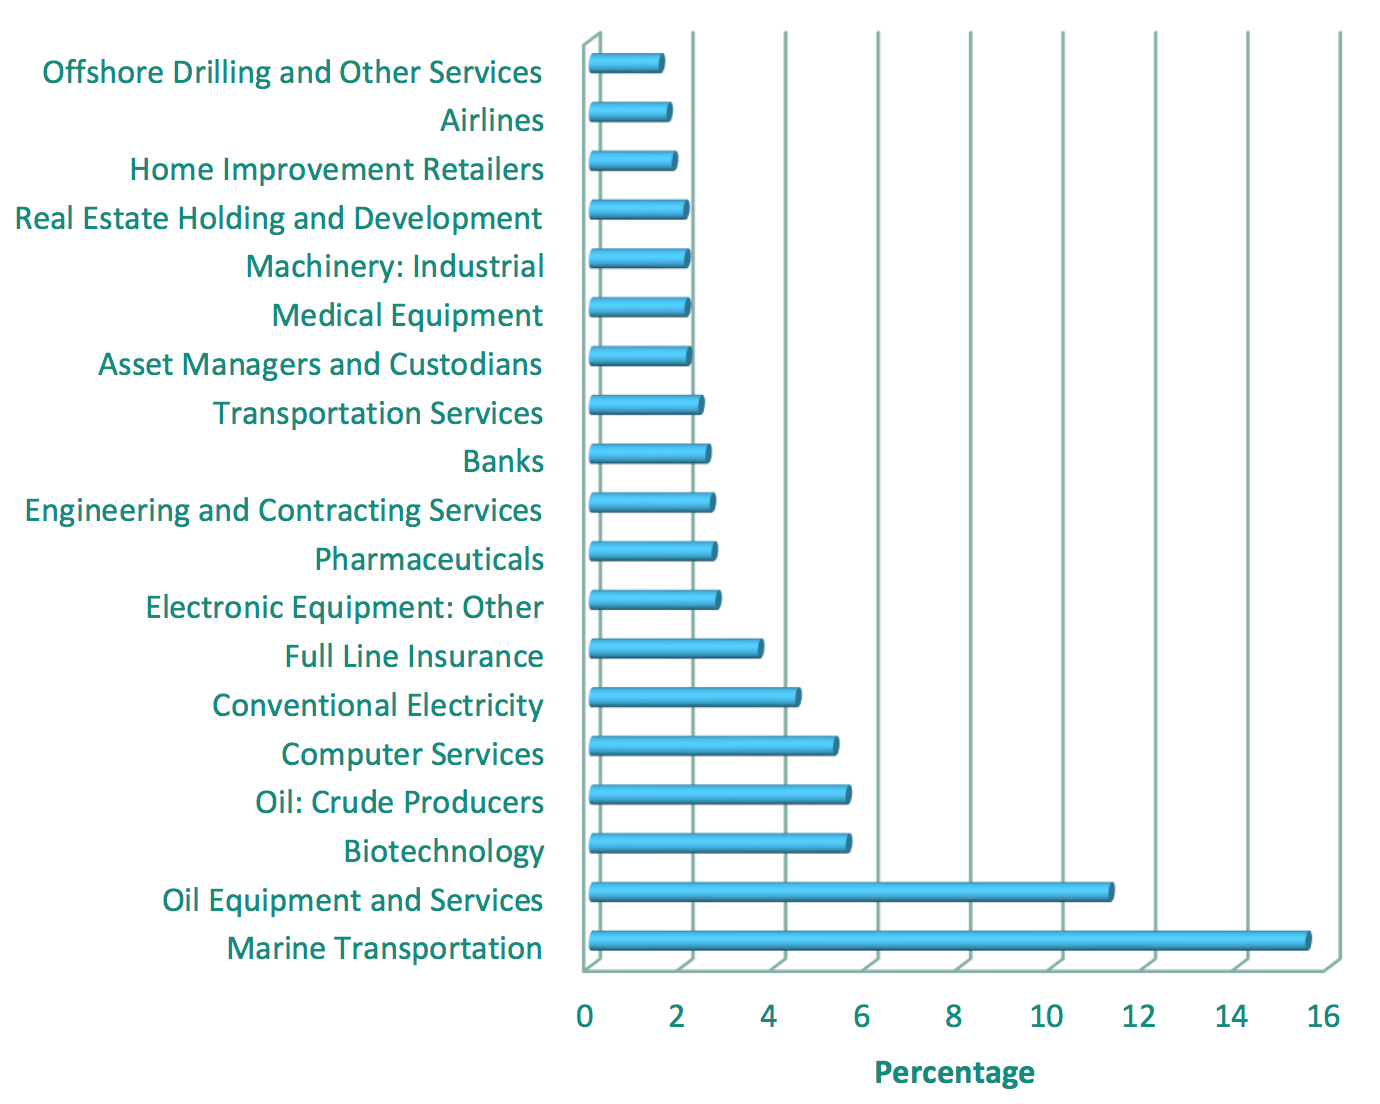
\includegraphics [scale=0.44,angle=360]{figures/smallsector.png}
\caption{OSESX Sector Allocation \cite{euronext}}
\label{fig:smallsector}
\end{figure}
\indent\newline 
Figure 3.1 shows the sector allocation of the small cap index as of 2021. The Index is dominated by marine transportation- and oil equipment and services companies, which accounts for approximately 25\% of the total index market cap. The smallest sectors consist of offshore drilling and airlines, and accounts for less than 2\% respectively of the total market cap. 

\indent\newline 
\begin{table}[ht]
\centering
\resizebox{\textwidth}{!}{\begin{tabular}{l|l}
\toprule
\textbf{Small cap statistics 2012-2020} \\ \midrule
Total number of stocks & 114 \\
Highest market capitalization & DOF Subsea (NOK 2,998,386,000 - 2012) \\
Lowest market capitalization & SeaBird Exploration (NOK 16,087,000 - 2017) \\
OSESX annualized returns  & 8.2\% \\ \bottomrule
\end{tabular}}
\caption{Small cap summary statistics}
\end{table}

\section{Large Cap}
\begin{figure}[H]
\centering
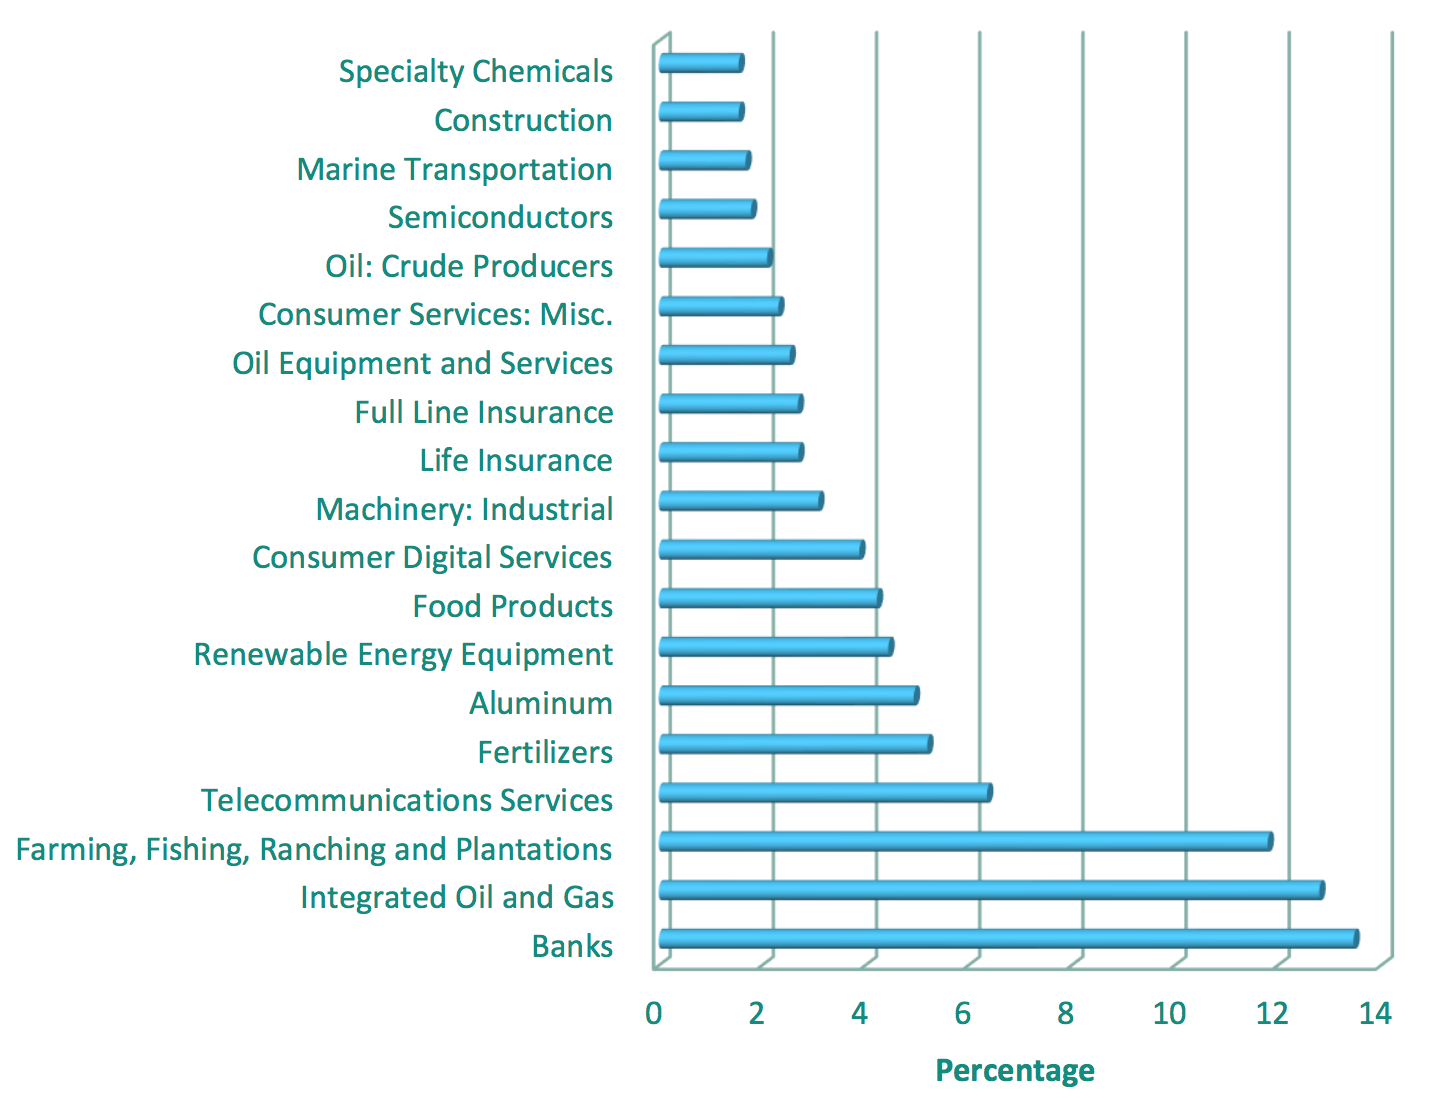
\includegraphics [scale=0.44,angle=360]{figures/largesector.png}
\caption{OSEBX Sector Allocation \cite{bors}}
\label{fig:largesector}
\end{figure}
\indent\newline 
Figure 3.2 illustrates the current sector allocation of the OSEBX index, mainly consisting of large cap stocks. The top three sectors are banks, integrated oil and gas, and farming, fishing, ranching and plantations, which represent approximately 38\% of the index total market cap. The bottom three sectors are specialty chemicals, construction, and marine transportation, where each sector makes up less than 2\% of the index. 

\indent\newline 
\begin{table}[ht]
\centering
\resizebox{\textwidth}{!}{\begin{tabular}{l|l}
\toprule
\textbf{Large cap statistics 2012-2020}  \\ \midrule
Total number of stocks & 64 \\
Highest market capitalization & Equinor (NOK 613,478,999,000 - 2018)  \\
Lowest market capitalization & Fjordkraft Holding (NOK 6,060,781,000 - 2019) \\
OSEBX annualized returns  & 16.7\% \\ \bottomrule
\end{tabular}}
\caption{Large cap summary statistics}
\end{table} 

\end{document}